\documentclass[a4paper,11pt]{article}
\usepackage[T1]{fontenc}
% \usepackage[utf8]{inputenc}
\usepackage{lmodern}

\usepackage{graphicx}
\usepackage[english]{babel}

\usepackage{listings} % package for listing parts of code

\usepackage{amsmath}
\usepackage{hyperref}

\usepackage{pgfplots}


% \renewcommand*\footnoterule{}

% \makeatletter
% \renewcommand{\@chapapp}{}% Not necessary...
% \newenvironment{chapquote}[2][2em]
%   {\setlength{\@tempdima}{#1}%
%    \def\chapquote@author{#2}%
%    \parshape 1 \@tempdima \dimexpr\textwidth-2\@tempdima\relax%
%    \itshape}
%   {\par\normalfont\hfill--\ \chapquote@author\hspace*{\@tempdima}\par\bigskip}
% \makeatother

% \def\subsubsectionfont{\fontfamily{\rmdefault}\fontshape{it}\selectfont\raggedright}
% % \newcounter {subsubsection}[subsection]
% % \newcounter {paragraph}[subsubsection]
% % \renewcommand\thesubsubsection{\thesubsection .\@arabic\c@subsubsection}
% % \renewcommand\theparagraph    {\thesubsubsection.\@arabic\c@paragraph}
% \newcommand\subsubsection{\@startsection{subsubsection}{3}{\z@}%
%                                     {-11pt \@plus -2\p@ \@minus -2\p@}%
%                                     {-.5em}%
%                                     {\subsubsectionfont}}
% % \newcommand*\l@subsubsection{\@dottedtocline{3}{3.8em}{3.2em}}


% Book's title and subtitle
\title{\Huge \textbf{High Performance Computing with Python} \vspace{4mm} \\ \huge Final Report}
% Author
% \author{\textsc{First-name Last-name}\footnote{email address}}
\author{\textsc{Jonas Manser} \\ \vspace{3mm}\text{4953222}  \\
\vspace{3mm}\text{jonas.burster@gmail.com}}


\begin{document}

\makeatletter
\begin{titlepage}
  \begin{center}
    
\includegraphics[width=0.5\linewidth]{logos/Uni_Logo-Grundversion_E1_A4_CMYK.eps}\\[4ex]
    {\huge \bfseries  \@title }\\[2ex]
    {\LARGE  \@author}\\[30ex]
    {\large \@date}
  \end{center}
\end{titlepage}
\makeatother
\thispagestyle{empty}
\newpage



\tableofcontents
\clearpage


\section{Introduction}
The Lattice Boltzmann Method (LBM) is a numerical solution of (nonlinear) partial differential equations of the original BLT introduced in 1988 by McNamara and Zanetti~\cite{mcnamara1988boltzmann-method}.
It is used to simulate flows in a closed system and is based on the core assumption that flows can be approximated to particles on a lattice.
This assumption has been shown to be true for incompressible subsonic flows of fluids and gases.
Today, the LBM is used in a wide variety of fields from car aerodynamics to ocean current flows.

The LBM originates from the lattice gas automata (LGA) pioneered by Hardy, Pomeau and de Pazzis in the 1970s with the HPP-model~\cite{hardy1973timeHPP}.
This model could be used to simluate both gas and fluid flows, but did not not, as initially hoped by the authors, lead to the Navier-Stokes equation in the macroscopic limit.
Later lattice gas automata models like the FPH-model~\cite{PhysRevLett.56.1505-fhp} were able to satisfy the Navier-Stokes equation but were still plagued by many problens, like the lack of Galilean invariance~\cite{nie2008galileanInvariance} or the strong assumption
that each node is surrounded by discrete particle cells, which resulted in massive computing requirements.
It also assumed that streaming and collision happened synchronously for all nodes and thus the collision was non-deterministic.

In 1988 McNamara and Zanetti introduced the LBM as a direct alternative to the LGA~\cite{mcnamara1988boltzmann-method}.
Their new method "is based on the simulation of a very simple microscopic system, rather than on the direct integration of partial differential equations"~\cite{mcnamara1988boltzmann-method}.
Because of their close similarity the LBM shares many features with the LGA, like the lack of Galilean invariance but it also satisfies the Navier-Stokes equation in the macroscopic limit.
It, crucially, "directly stud[ies] the time evolution of the mean values"~\cite{mcnamara1988boltzmann-method} and thus does not need statistical averaging to compute the velocity as in LGA leading to lower computing requirements.

The key points of the LBM success is it's simplicity, relatively low consumption of computing requirements and easy parallelization of the algorithm.
This is achieved by approximating the fluid to particles on a grid and using a separate streaming and collision step to simulate the particles behaviour over time.
This is unlike other computational fluid dynamics (CFD) methods which directly solve the numerically macroscopic properties of a fluied, i.e. the mass, momentum, and energy.
Using particles also makes incorperating boundries and microscopic interactions easier than in most other CFD models.

The reminder of the report will first introduce the theory behind the LBM and later present the results for each milestone.

\section{Theoretical background}
\subsection{Probability Density Function}
The probability density function (PDF) describes the statistical probability of particles in a closed system not in equilibrium and is denoted by $f$.
In this case, the PDF is given by $f(r_i,v_i,t)$ where $r$ are the positions and $v$ the velocities.
The probability for finding a particle in a certain part of the phase space is then given by equation~\ref{eq:pdf}.
\begin{equation}
  \label{eq:pdf}
  \begin{aligned}
    dP = f(\vec{r},\vec{v},t) d^{3}\vec{r} d^{3}\vec{v}
  \end{aligned}
\end{equation}
The phase space for equation \href{eq:pdf} is given by $[\vec{r}, \vec{r}+d\vec{r}, \vec{v}, \vec{v}+d\vec{v}]$.
Thus, the probability for finding a particle in the phase space at position $r_i$ is only depended on the velocity $v_i$ and time $t$.

The probability of finding a single particle with an arbitraty place $r$ and an arbitrary velocity $v$ in the entire phase space is given by equation \ref{eq:prob-single}.
\begin{equation}
  \label{eq:prob-single}
  \begin{aligned}
    P = \int_{\Omega_{\vec{r}}} \int_{\Omega_{\vec{v}}}  f(\vec{r},\vec{v},t) d^{3}\vec{r} d^{3}\vec{v} \quad \overset{!}{=} 1
  \end{aligned}
\end{equation}
As we are in a closed system where no particles are added or destroyed we can assume that it must hold that equation \href{eq:prob-single} is equal to one, i.e. normalized to unity.

This then leads us to the general form of the $i$-th moments of $ f(\vec{r},\vec{v},t) $ w.r.t. $ \vec{v} $ shown in equation \ref{eq:general-moments}.
\begin{equation}
  \label{eq:general-moments}
  \begin{aligned}
    \mu_{i}(\vec{r}) =\int_{\Omega_{\vec{v}}}\vec{v}^{i} f(\vec{r},\vec{v},t)d^{3}\vec{v}
  \end{aligned}
\end{equation}
The first and second order moments are the main subjects of this project and can be readily interpreted.
The first order moment is the velocity in our system, which for liquids is the flow field.
The second order moment is the kenetic energy density in our system which can be readily interpreted as the temperature of a fluid.
Different fluids can have different translation ratios between velocities and temperature and thus an increase in temperature in a closed system would lead to higher velocities but the exact increase is depended on the fluid.


\subsection{Boltzmann Transport Equation}
The Boltzmann transport equation (BTE) tracks the time evolution of the probability distribution function and was published by Ludwig Boltzmann in 1872.
To derive it we take the first order derivative of the PDF in respect to time as shown in
equation \ref{eq:BTE}.
\begin{equation}
  \label{eq:BTE}
  \begin{aligned}
    \frac{df}{dt} =\frac{\partial f}{\partial t} + \frac{dr(t)}{dt} \nabla_{r}f + \frac{dv(t)}{dt} \nabla_{v}f = \left( \frac{\partial f}{\partial t} \right)_{col}
  \end{aligned}
\end{equation}
Where the term $f$ is the PDF, $\frac{dr(t)}{dt}$ is called the velocity and $\frac{dv(t)}{dt}$ is called the acceleration and by Newtons law is the force acting on the particles devivded by their respective mass.
The \textit{l.h.s.} of equation \ref{eq:BTE} is called the streaming term and the \textit{r.h.s} is the collision term.
To show an implementation of the streaming and collision terms the BTE first needs to be discretized.




\subsection{Lattice-Boltzmann Method} \label{sec:lbm}
The BTE is defined in a continous phase space which is not readily implementable in computer code.
This can be overcome by approximating the continous phase space to a discrete phase space, called the Lattice-Boltzmann method (LBM).
The idea is to discretize over a lattice and use the partial derivatives to solve the BTE.
In this project the the spatial dimension is discretized to a 2D lattice and the velocities are descritized to 9 directions also called a D2Q9-model.
This is illustarate in \href{fig:d2q9-scheme} where $a$ shows the discretazation of the velocity space and $b$ the discretized of the physical space on a 2D grid with the velocity layered on top.
\begin{figure}[h]
  \caption{Discretization of the BTE.}
  \label{fig:d2q9-scheme}
  \centering
  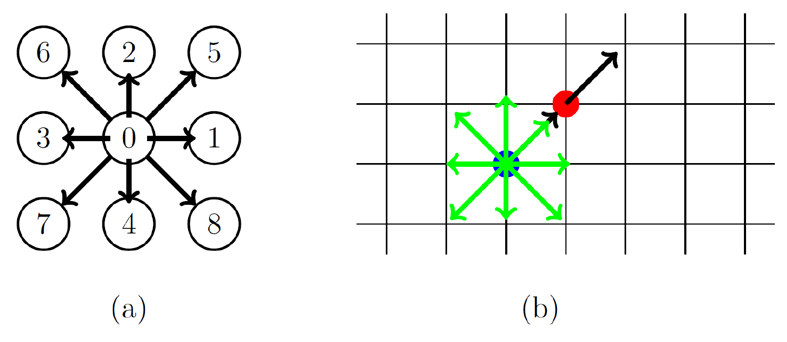
\includegraphics[width=9cm]{d2q9_scheme.png}\\
  (a) Discretization on the velocity space according to D2Q9.\\
  (b) Uniform 2D grid for the discretization in the physical space.\\
  \small{(Material from lecture)}
\end{figure}

\clearpage
\section{Milestons}
This chapter presents the results from the seven milestone and gives an in detail review.

\subsection{M1: Streaming}
As shown in equation~\ref{eq:pdf} streaming and collision are two separate terms.
The collision can be ignored by setting it to zero, i.e. $\left( \frac{\partial f}{\partial t} \right)_{col} \overset{!}{=} 0$.
This simplifies the BTE and implies the movement of particles in the vacuum with no mutual interaction between particles and is defined by equation \ref{eq:streaming}.
\begin{equation}
  \label{eq:streaming}
  \begin{aligned}
    f_{i}(r+c_{i} \nabla t,t+\nabla t)=f_{i}(r,t)
  \end{aligned}
\end{equation}
The code implementation of a streaming function on a 2D lattice is shown in listing \ref{lst:streaming}
\footnote{Throughout I will use the notation $_ixy$ where $i$ is the rolling dimension and x and y are the deminsions of the physical space.}.
\begin{center}
\begin{lstlisting}[caption=Implementation of the streaming operator,label=lst:streaming, basicstyle=\small]
def stream(f_cxy: np.array) -> np.array:
    for i in range(1, 9):
        f_cxy[i, :, :] = np.roll(f_cxy[i, :, :], 
                      shift=C_CA[i], 
                      axis=(0, 1))
    return f_cxy
  \end{lstlisting}
\end{center}
Where $f_{cxy}$ is the PDF and $C \_ CA$ are the discretized velocity directions.
For each velocity direction the streaming shifts the velocities values in the respective direction.
Testing the streaming operator can be easily done by visualizing the different shift on a 2D grid for each velocity as shown in figure \ref{fig:m1-shifting} for the velocities $v=2$ $v=3$.
\begin{figure}[ht]
\centering
\resizebox{\columnwidth}{!}{\large%% Creator: Matplotlib, PGF backend
%%
%% To include the figure in your LaTeX document, write
%%   \input{<filename>.pgf}
%%
%% Make sure the required packages are loaded in your preamble
%%   \usepackage{pgf}
%%
%% Also ensure that all the required font packages are loaded; for instance,
%% the lmodern package is sometimes necessary when using math font.
%%   \usepackage{lmodern}
%%
%% Figures using additional raster images can only be included by \input if
%% they are in the same directory as the main LaTeX file. For loading figures
%% from other directories you can use the `import` package
%%   \usepackage{import}
%%
%% and then include the figures with
%%   \import{<path to file>}{<filename>.pgf}
%%
%% Matplotlib used the following preamble
%%   \usepackage{fontspec}
%%   \setmainfont{DejaVuSerif.ttf}[Path=\detokenize{/home/joe/miniconda3/envs/high/lib/python3.9/site-packages/matplotlib/mpl-data/fonts/ttf/}]
%%   \setsansfont{DejaVuSans.ttf}[Path=\detokenize{/home/joe/miniconda3/envs/high/lib/python3.9/site-packages/matplotlib/mpl-data/fonts/ttf/}]
%%   \setmonofont{DejaVuSansMono.ttf}[Path=\detokenize{/home/joe/miniconda3/envs/high/lib/python3.9/site-packages/matplotlib/mpl-data/fonts/ttf/}]
%%
\begingroup%
\makeatletter%
\begin{pgfpicture}%
\pgfpathrectangle{\pgfpointorigin}{\pgfqpoint{15.000000in}{5.000000in}}%
\pgfusepath{use as bounding box, clip}%
\begin{pgfscope}%
\pgfsetbuttcap%
\pgfsetmiterjoin%
\pgfsetlinewidth{0.000000pt}%
\definecolor{currentstroke}{rgb}{1.000000,1.000000,1.000000}%
\pgfsetstrokecolor{currentstroke}%
\pgfsetstrokeopacity{0.000000}%
\pgfsetdash{}{0pt}%
\pgfpathmoveto{\pgfqpoint{0.000000in}{0.000000in}}%
\pgfpathlineto{\pgfqpoint{15.000000in}{0.000000in}}%
\pgfpathlineto{\pgfqpoint{15.000000in}{5.000000in}}%
\pgfpathlineto{\pgfqpoint{0.000000in}{5.000000in}}%
\pgfpathlineto{\pgfqpoint{0.000000in}{0.000000in}}%
\pgfpathclose%
\pgfusepath{}%
\end{pgfscope}%
\begin{pgfscope}%
\pgfsetbuttcap%
\pgfsetmiterjoin%
\definecolor{currentfill}{rgb}{1.000000,1.000000,1.000000}%
\pgfsetfillcolor{currentfill}%
\pgfsetlinewidth{0.000000pt}%
\definecolor{currentstroke}{rgb}{0.000000,0.000000,0.000000}%
\pgfsetstrokecolor{currentstroke}%
\pgfsetstrokeopacity{0.000000}%
\pgfsetdash{}{0pt}%
\pgfpathmoveto{\pgfqpoint{0.794097in}{3.269444in}}%
\pgfpathlineto{\pgfqpoint{3.712500in}{3.269444in}}%
\pgfpathlineto{\pgfqpoint{3.712500in}{4.850000in}}%
\pgfpathlineto{\pgfqpoint{0.794097in}{4.850000in}}%
\pgfpathlineto{\pgfqpoint{0.794097in}{3.269444in}}%
\pgfpathclose%
\pgfusepath{fill}%
\end{pgfscope}%
\begin{pgfscope}%
\pgfpathrectangle{\pgfqpoint{0.794097in}{3.269444in}}{\pgfqpoint{2.918403in}{1.580556in}}%
\pgfusepath{clip}%
\pgfsetbuttcap%
\pgfsetroundjoin%
\definecolor{currentfill}{rgb}{0.984744,0.432910,0.307420}%
\pgfsetfillcolor{currentfill}%
\pgfsetlinewidth{0.000000pt}%
\definecolor{currentstroke}{rgb}{0.000000,0.000000,0.000000}%
\pgfsetstrokecolor{currentstroke}%
\pgfsetdash{}{0pt}%
\pgfpathmoveto{\pgfqpoint{0.794097in}{3.269444in}}%
\pgfpathlineto{\pgfqpoint{0.794097in}{3.664583in}}%
\pgfpathlineto{\pgfqpoint{1.377778in}{3.664583in}}%
\pgfpathlineto{\pgfqpoint{1.377778in}{3.269444in}}%
\pgfpathlineto{\pgfqpoint{0.794097in}{3.269444in}}%
\pgfpathlineto{\pgfqpoint{0.794097in}{3.269444in}}%
\pgfpathclose%
\pgfusepath{fill}%
\end{pgfscope}%
\begin{pgfscope}%
\pgfpathrectangle{\pgfqpoint{0.794097in}{3.269444in}}{\pgfqpoint{2.918403in}{1.580556in}}%
\pgfusepath{clip}%
\pgfsetbuttcap%
\pgfsetroundjoin%
\definecolor{currentfill}{rgb}{0.974717,0.378101,0.266205}%
\pgfsetfillcolor{currentfill}%
\pgfsetlinewidth{0.000000pt}%
\definecolor{currentstroke}{rgb}{0.000000,0.000000,0.000000}%
\pgfsetstrokecolor{currentstroke}%
\pgfsetdash{}{0pt}%
\pgfpathmoveto{\pgfqpoint{1.377778in}{3.269444in}}%
\pgfpathlineto{\pgfqpoint{1.377778in}{3.664583in}}%
\pgfpathlineto{\pgfqpoint{1.961458in}{3.664583in}}%
\pgfpathlineto{\pgfqpoint{1.961458in}{3.269444in}}%
\pgfpathlineto{\pgfqpoint{1.377778in}{3.269444in}}%
\pgfpathlineto{\pgfqpoint{1.377778in}{3.269444in}}%
\pgfpathclose%
\pgfusepath{fill}%
\end{pgfscope}%
\begin{pgfscope}%
\pgfpathrectangle{\pgfqpoint{0.794097in}{3.269444in}}{\pgfqpoint{2.918403in}{1.580556in}}%
\pgfusepath{clip}%
\pgfsetbuttcap%
\pgfsetroundjoin%
\definecolor{currentfill}{rgb}{0.988235,0.681630,0.572103}%
\pgfsetfillcolor{currentfill}%
\pgfsetlinewidth{0.000000pt}%
\definecolor{currentstroke}{rgb}{0.000000,0.000000,0.000000}%
\pgfsetstrokecolor{currentstroke}%
\pgfsetdash{}{0pt}%
\pgfpathmoveto{\pgfqpoint{1.961458in}{3.269444in}}%
\pgfpathlineto{\pgfqpoint{1.961458in}{3.664583in}}%
\pgfpathlineto{\pgfqpoint{2.545139in}{3.664583in}}%
\pgfpathlineto{\pgfqpoint{2.545139in}{3.269444in}}%
\pgfpathlineto{\pgfqpoint{1.961458in}{3.269444in}}%
\pgfpathlineto{\pgfqpoint{1.961458in}{3.269444in}}%
\pgfpathclose%
\pgfusepath{fill}%
\end{pgfscope}%
\begin{pgfscope}%
\pgfpathrectangle{\pgfqpoint{0.794097in}{3.269444in}}{\pgfqpoint{2.918403in}{1.580556in}}%
\pgfusepath{clip}%
\pgfsetbuttcap%
\pgfsetroundjoin%
\definecolor{currentfill}{rgb}{0.525967,0.029527,0.066728}%
\pgfsetfillcolor{currentfill}%
\pgfsetlinewidth{0.000000pt}%
\definecolor{currentstroke}{rgb}{0.000000,0.000000,0.000000}%
\pgfsetstrokecolor{currentstroke}%
\pgfsetdash{}{0pt}%
\pgfpathmoveto{\pgfqpoint{2.545139in}{3.269444in}}%
\pgfpathlineto{\pgfqpoint{2.545139in}{3.664583in}}%
\pgfpathlineto{\pgfqpoint{3.128819in}{3.664583in}}%
\pgfpathlineto{\pgfqpoint{3.128819in}{3.269444in}}%
\pgfpathlineto{\pgfqpoint{2.545139in}{3.269444in}}%
\pgfpathlineto{\pgfqpoint{2.545139in}{3.269444in}}%
\pgfpathclose%
\pgfusepath{fill}%
\end{pgfscope}%
\begin{pgfscope}%
\pgfpathrectangle{\pgfqpoint{0.794097in}{3.269444in}}{\pgfqpoint{2.918403in}{1.580556in}}%
\pgfusepath{clip}%
\pgfsetbuttcap%
\pgfsetroundjoin%
\definecolor{currentfill}{rgb}{0.525967,0.029527,0.066728}%
\pgfsetfillcolor{currentfill}%
\pgfsetlinewidth{0.000000pt}%
\definecolor{currentstroke}{rgb}{0.000000,0.000000,0.000000}%
\pgfsetstrokecolor{currentstroke}%
\pgfsetdash{}{0pt}%
\pgfpathmoveto{\pgfqpoint{3.128819in}{3.269444in}}%
\pgfpathlineto{\pgfqpoint{3.128819in}{3.664583in}}%
\pgfpathlineto{\pgfqpoint{3.712500in}{3.664583in}}%
\pgfpathlineto{\pgfqpoint{3.712500in}{3.269444in}}%
\pgfpathlineto{\pgfqpoint{3.128819in}{3.269444in}}%
\pgfpathlineto{\pgfqpoint{3.128819in}{3.269444in}}%
\pgfpathclose%
\pgfusepath{fill}%
\end{pgfscope}%
\begin{pgfscope}%
\pgfpathrectangle{\pgfqpoint{0.794097in}{3.269444in}}{\pgfqpoint{2.918403in}{1.580556in}}%
\pgfusepath{clip}%
\pgfsetbuttcap%
\pgfsetroundjoin%
\definecolor{currentfill}{rgb}{0.974717,0.378101,0.266205}%
\pgfsetfillcolor{currentfill}%
\pgfsetlinewidth{0.000000pt}%
\definecolor{currentstroke}{rgb}{0.000000,0.000000,0.000000}%
\pgfsetstrokecolor{currentstroke}%
\pgfsetdash{}{0pt}%
\pgfpathmoveto{\pgfqpoint{0.794097in}{3.664583in}}%
\pgfpathlineto{\pgfqpoint{0.794097in}{4.059722in}}%
\pgfpathlineto{\pgfqpoint{1.377778in}{4.059722in}}%
\pgfpathlineto{\pgfqpoint{1.377778in}{3.664583in}}%
\pgfpathlineto{\pgfqpoint{0.794097in}{3.664583in}}%
\pgfpathlineto{\pgfqpoint{0.794097in}{3.664583in}}%
\pgfpathclose%
\pgfusepath{fill}%
\end{pgfscope}%
\begin{pgfscope}%
\pgfpathrectangle{\pgfqpoint{0.794097in}{3.269444in}}{\pgfqpoint{2.918403in}{1.580556in}}%
\pgfusepath{clip}%
\pgfsetbuttcap%
\pgfsetroundjoin%
\definecolor{currentfill}{rgb}{0.640384,0.057209,0.081492}%
\pgfsetfillcolor{currentfill}%
\pgfsetlinewidth{0.000000pt}%
\definecolor{currentstroke}{rgb}{0.000000,0.000000,0.000000}%
\pgfsetstrokecolor{currentstroke}%
\pgfsetdash{}{0pt}%
\pgfpathmoveto{\pgfqpoint{1.377778in}{3.664583in}}%
\pgfpathlineto{\pgfqpoint{1.377778in}{4.059722in}}%
\pgfpathlineto{\pgfqpoint{1.961458in}{4.059722in}}%
\pgfpathlineto{\pgfqpoint{1.961458in}{3.664583in}}%
\pgfpathlineto{\pgfqpoint{1.377778in}{3.664583in}}%
\pgfpathlineto{\pgfqpoint{1.377778in}{3.664583in}}%
\pgfpathclose%
\pgfusepath{fill}%
\end{pgfscope}%
\begin{pgfscope}%
\pgfpathrectangle{\pgfqpoint{0.794097in}{3.269444in}}{\pgfqpoint{2.918403in}{1.580556in}}%
\pgfusepath{clip}%
\pgfsetbuttcap%
\pgfsetroundjoin%
\definecolor{currentfill}{rgb}{0.948143,0.274018,0.199769}%
\pgfsetfillcolor{currentfill}%
\pgfsetlinewidth{0.000000pt}%
\definecolor{currentstroke}{rgb}{0.000000,0.000000,0.000000}%
\pgfsetstrokecolor{currentstroke}%
\pgfsetdash{}{0pt}%
\pgfpathmoveto{\pgfqpoint{1.961458in}{3.664583in}}%
\pgfpathlineto{\pgfqpoint{1.961458in}{4.059722in}}%
\pgfpathlineto{\pgfqpoint{2.545139in}{4.059722in}}%
\pgfpathlineto{\pgfqpoint{2.545139in}{3.664583in}}%
\pgfpathlineto{\pgfqpoint{1.961458in}{3.664583in}}%
\pgfpathlineto{\pgfqpoint{1.961458in}{3.664583in}}%
\pgfpathclose%
\pgfusepath{fill}%
\end{pgfscope}%
\begin{pgfscope}%
\pgfpathrectangle{\pgfqpoint{0.794097in}{3.269444in}}{\pgfqpoint{2.918403in}{1.580556in}}%
\pgfusepath{clip}%
\pgfsetbuttcap%
\pgfsetroundjoin%
\definecolor{currentfill}{rgb}{0.666344,0.063391,0.086413}%
\pgfsetfillcolor{currentfill}%
\pgfsetlinewidth{0.000000pt}%
\definecolor{currentstroke}{rgb}{0.000000,0.000000,0.000000}%
\pgfsetstrokecolor{currentstroke}%
\pgfsetdash{}{0pt}%
\pgfpathmoveto{\pgfqpoint{2.545139in}{3.664583in}}%
\pgfpathlineto{\pgfqpoint{2.545139in}{4.059722in}}%
\pgfpathlineto{\pgfqpoint{3.128819in}{4.059722in}}%
\pgfpathlineto{\pgfqpoint{3.128819in}{3.664583in}}%
\pgfpathlineto{\pgfqpoint{2.545139in}{3.664583in}}%
\pgfpathlineto{\pgfqpoint{2.545139in}{3.664583in}}%
\pgfpathclose%
\pgfusepath{fill}%
\end{pgfscope}%
\begin{pgfscope}%
\pgfpathrectangle{\pgfqpoint{0.794097in}{3.269444in}}{\pgfqpoint{2.918403in}{1.580556in}}%
\pgfusepath{clip}%
\pgfsetbuttcap%
\pgfsetroundjoin%
\definecolor{currentfill}{rgb}{0.988235,0.666498,0.554756}%
\pgfsetfillcolor{currentfill}%
\pgfsetlinewidth{0.000000pt}%
\definecolor{currentstroke}{rgb}{0.000000,0.000000,0.000000}%
\pgfsetstrokecolor{currentstroke}%
\pgfsetdash{}{0pt}%
\pgfpathmoveto{\pgfqpoint{3.128819in}{3.664583in}}%
\pgfpathlineto{\pgfqpoint{3.128819in}{4.059722in}}%
\pgfpathlineto{\pgfqpoint{3.712500in}{4.059722in}}%
\pgfpathlineto{\pgfqpoint{3.712500in}{3.664583in}}%
\pgfpathlineto{\pgfqpoint{3.128819in}{3.664583in}}%
\pgfpathlineto{\pgfqpoint{3.128819in}{3.664583in}}%
\pgfpathclose%
\pgfusepath{fill}%
\end{pgfscope}%
\begin{pgfscope}%
\pgfpathrectangle{\pgfqpoint{0.794097in}{3.269444in}}{\pgfqpoint{2.918403in}{1.580556in}}%
\pgfusepath{clip}%
\pgfsetbuttcap%
\pgfsetroundjoin%
\definecolor{currentfill}{rgb}{0.954048,0.297147,0.214533}%
\pgfsetfillcolor{currentfill}%
\pgfsetlinewidth{0.000000pt}%
\definecolor{currentstroke}{rgb}{0.000000,0.000000,0.000000}%
\pgfsetstrokecolor{currentstroke}%
\pgfsetdash{}{0pt}%
\pgfpathmoveto{\pgfqpoint{0.794097in}{4.059722in}}%
\pgfpathlineto{\pgfqpoint{0.794097in}{4.454861in}}%
\pgfpathlineto{\pgfqpoint{1.377778in}{4.454861in}}%
\pgfpathlineto{\pgfqpoint{1.377778in}{4.059722in}}%
\pgfpathlineto{\pgfqpoint{0.794097in}{4.059722in}}%
\pgfpathlineto{\pgfqpoint{0.794097in}{4.059722in}}%
\pgfpathclose%
\pgfusepath{fill}%
\end{pgfscope}%
\begin{pgfscope}%
\pgfpathrectangle{\pgfqpoint{0.794097in}{3.269444in}}{\pgfqpoint{2.918403in}{1.580556in}}%
\pgfusepath{clip}%
\pgfsetbuttcap%
\pgfsetroundjoin%
\definecolor{currentfill}{rgb}{0.988189,0.570704,0.445213}%
\pgfsetfillcolor{currentfill}%
\pgfsetlinewidth{0.000000pt}%
\definecolor{currentstroke}{rgb}{0.000000,0.000000,0.000000}%
\pgfsetstrokecolor{currentstroke}%
\pgfsetdash{}{0pt}%
\pgfpathmoveto{\pgfqpoint{1.377778in}{4.059722in}}%
\pgfpathlineto{\pgfqpoint{1.377778in}{4.454861in}}%
\pgfpathlineto{\pgfqpoint{1.961458in}{4.454861in}}%
\pgfpathlineto{\pgfqpoint{1.961458in}{4.059722in}}%
\pgfpathlineto{\pgfqpoint{1.377778in}{4.059722in}}%
\pgfpathlineto{\pgfqpoint{1.377778in}{4.059722in}}%
\pgfpathclose%
\pgfusepath{fill}%
\end{pgfscope}%
\begin{pgfscope}%
\pgfpathrectangle{\pgfqpoint{0.794097in}{3.269444in}}{\pgfqpoint{2.918403in}{1.580556in}}%
\pgfusepath{clip}%
\pgfsetbuttcap%
\pgfsetroundjoin%
\definecolor{currentfill}{rgb}{0.961430,0.326059,0.232987}%
\pgfsetfillcolor{currentfill}%
\pgfsetlinewidth{0.000000pt}%
\definecolor{currentstroke}{rgb}{0.000000,0.000000,0.000000}%
\pgfsetstrokecolor{currentstroke}%
\pgfsetdash{}{0pt}%
\pgfpathmoveto{\pgfqpoint{1.961458in}{4.059722in}}%
\pgfpathlineto{\pgfqpoint{1.961458in}{4.454861in}}%
\pgfpathlineto{\pgfqpoint{2.545139in}{4.454861in}}%
\pgfpathlineto{\pgfqpoint{2.545139in}{4.059722in}}%
\pgfpathlineto{\pgfqpoint{1.961458in}{4.059722in}}%
\pgfpathlineto{\pgfqpoint{1.961458in}{4.059722in}}%
\pgfpathclose%
\pgfusepath{fill}%
\end{pgfscope}%
\begin{pgfscope}%
\pgfpathrectangle{\pgfqpoint{0.794097in}{3.269444in}}{\pgfqpoint{2.918403in}{1.580556in}}%
\pgfusepath{clip}%
\pgfsetbuttcap%
\pgfsetroundjoin%
\definecolor{currentfill}{rgb}{0.990388,0.773164,0.684121}%
\pgfsetfillcolor{currentfill}%
\pgfsetlinewidth{0.000000pt}%
\definecolor{currentstroke}{rgb}{0.000000,0.000000,0.000000}%
\pgfsetstrokecolor{currentstroke}%
\pgfsetdash{}{0pt}%
\pgfpathmoveto{\pgfqpoint{2.545139in}{4.059722in}}%
\pgfpathlineto{\pgfqpoint{2.545139in}{4.454861in}}%
\pgfpathlineto{\pgfqpoint{3.128819in}{4.454861in}}%
\pgfpathlineto{\pgfqpoint{3.128819in}{4.059722in}}%
\pgfpathlineto{\pgfqpoint{2.545139in}{4.059722in}}%
\pgfpathlineto{\pgfqpoint{2.545139in}{4.059722in}}%
\pgfpathclose%
\pgfusepath{fill}%
\end{pgfscope}%
\begin{pgfscope}%
\pgfpathrectangle{\pgfqpoint{0.794097in}{3.269444in}}{\pgfqpoint{2.918403in}{1.580556in}}%
\pgfusepath{clip}%
\pgfsetbuttcap%
\pgfsetroundjoin%
\definecolor{currentfill}{rgb}{0.988235,0.575702,0.450673}%
\pgfsetfillcolor{currentfill}%
\pgfsetlinewidth{0.000000pt}%
\definecolor{currentstroke}{rgb}{0.000000,0.000000,0.000000}%
\pgfsetstrokecolor{currentstroke}%
\pgfsetdash{}{0pt}%
\pgfpathmoveto{\pgfqpoint{3.128819in}{4.059722in}}%
\pgfpathlineto{\pgfqpoint{3.128819in}{4.454861in}}%
\pgfpathlineto{\pgfqpoint{3.712500in}{4.454861in}}%
\pgfpathlineto{\pgfqpoint{3.712500in}{4.059722in}}%
\pgfpathlineto{\pgfqpoint{3.128819in}{4.059722in}}%
\pgfpathlineto{\pgfqpoint{3.128819in}{4.059722in}}%
\pgfpathclose%
\pgfusepath{fill}%
\end{pgfscope}%
\begin{pgfscope}%
\pgfpathrectangle{\pgfqpoint{0.794097in}{3.269444in}}{\pgfqpoint{2.918403in}{1.580556in}}%
\pgfusepath{clip}%
\pgfsetbuttcap%
\pgfsetroundjoin%
\definecolor{currentfill}{rgb}{0.991373,0.791373,0.708235}%
\pgfsetfillcolor{currentfill}%
\pgfsetlinewidth{0.000000pt}%
\definecolor{currentstroke}{rgb}{0.000000,0.000000,0.000000}%
\pgfsetstrokecolor{currentstroke}%
\pgfsetdash{}{0pt}%
\pgfpathmoveto{\pgfqpoint{0.794097in}{4.454861in}}%
\pgfpathlineto{\pgfqpoint{0.794097in}{4.850000in}}%
\pgfpathlineto{\pgfqpoint{1.377778in}{4.850000in}}%
\pgfpathlineto{\pgfqpoint{1.377778in}{4.454861in}}%
\pgfpathlineto{\pgfqpoint{0.794097in}{4.454861in}}%
\pgfpathlineto{\pgfqpoint{0.794097in}{4.454861in}}%
\pgfpathclose%
\pgfusepath{fill}%
\end{pgfscope}%
\begin{pgfscope}%
\pgfpathrectangle{\pgfqpoint{0.794097in}{3.269444in}}{\pgfqpoint{2.918403in}{1.580556in}}%
\pgfusepath{clip}%
\pgfsetbuttcap%
\pgfsetroundjoin%
\definecolor{currentfill}{rgb}{0.985729,0.472280,0.346790}%
\pgfsetfillcolor{currentfill}%
\pgfsetlinewidth{0.000000pt}%
\definecolor{currentstroke}{rgb}{0.000000,0.000000,0.000000}%
\pgfsetstrokecolor{currentstroke}%
\pgfsetdash{}{0pt}%
\pgfpathmoveto{\pgfqpoint{1.377778in}{4.454861in}}%
\pgfpathlineto{\pgfqpoint{1.377778in}{4.850000in}}%
\pgfpathlineto{\pgfqpoint{1.961458in}{4.850000in}}%
\pgfpathlineto{\pgfqpoint{1.961458in}{4.454861in}}%
\pgfpathlineto{\pgfqpoint{1.377778in}{4.454861in}}%
\pgfpathlineto{\pgfqpoint{1.377778in}{4.454861in}}%
\pgfpathclose%
\pgfusepath{fill}%
\end{pgfscope}%
\begin{pgfscope}%
\pgfpathrectangle{\pgfqpoint{0.794097in}{3.269444in}}{\pgfqpoint{2.918403in}{1.580556in}}%
\pgfusepath{clip}%
\pgfsetbuttcap%
\pgfsetroundjoin%
\definecolor{currentfill}{rgb}{0.868051,0.164091,0.143714}%
\pgfsetfillcolor{currentfill}%
\pgfsetlinewidth{0.000000pt}%
\definecolor{currentstroke}{rgb}{0.000000,0.000000,0.000000}%
\pgfsetstrokecolor{currentstroke}%
\pgfsetdash{}{0pt}%
\pgfpathmoveto{\pgfqpoint{1.961458in}{4.454861in}}%
\pgfpathlineto{\pgfqpoint{1.961458in}{4.850000in}}%
\pgfpathlineto{\pgfqpoint{2.545139in}{4.850000in}}%
\pgfpathlineto{\pgfqpoint{2.545139in}{4.454861in}}%
\pgfpathlineto{\pgfqpoint{1.961458in}{4.454861in}}%
\pgfpathlineto{\pgfqpoint{1.961458in}{4.454861in}}%
\pgfpathclose%
\pgfusepath{fill}%
\end{pgfscope}%
\begin{pgfscope}%
\pgfpathrectangle{\pgfqpoint{0.794097in}{3.269444in}}{\pgfqpoint{2.918403in}{1.580556in}}%
\pgfusepath{clip}%
\pgfsetbuttcap%
\pgfsetroundjoin%
\definecolor{currentfill}{rgb}{1.000000,0.960784,0.941176}%
\pgfsetfillcolor{currentfill}%
\pgfsetlinewidth{0.000000pt}%
\definecolor{currentstroke}{rgb}{0.000000,0.000000,0.000000}%
\pgfsetstrokecolor{currentstroke}%
\pgfsetdash{}{0pt}%
\pgfpathmoveto{\pgfqpoint{2.545139in}{4.454861in}}%
\pgfpathlineto{\pgfqpoint{2.545139in}{4.850000in}}%
\pgfpathlineto{\pgfqpoint{3.128819in}{4.850000in}}%
\pgfpathlineto{\pgfqpoint{3.128819in}{4.454861in}}%
\pgfpathlineto{\pgfqpoint{2.545139in}{4.454861in}}%
\pgfpathlineto{\pgfqpoint{2.545139in}{4.454861in}}%
\pgfpathclose%
\pgfusepath{fill}%
\end{pgfscope}%
\begin{pgfscope}%
\pgfpathrectangle{\pgfqpoint{0.794097in}{3.269444in}}{\pgfqpoint{2.918403in}{1.580556in}}%
\pgfusepath{clip}%
\pgfsetbuttcap%
\pgfsetroundjoin%
\definecolor{currentfill}{rgb}{0.403922,0.000000,0.050980}%
\pgfsetfillcolor{currentfill}%
\pgfsetlinewidth{0.000000pt}%
\definecolor{currentstroke}{rgb}{0.000000,0.000000,0.000000}%
\pgfsetstrokecolor{currentstroke}%
\pgfsetdash{}{0pt}%
\pgfpathmoveto{\pgfqpoint{3.128819in}{4.454861in}}%
\pgfpathlineto{\pgfqpoint{3.128819in}{4.850000in}}%
\pgfpathlineto{\pgfqpoint{3.712500in}{4.850000in}}%
\pgfpathlineto{\pgfqpoint{3.712500in}{4.454861in}}%
\pgfpathlineto{\pgfqpoint{3.128819in}{4.454861in}}%
\pgfpathlineto{\pgfqpoint{3.128819in}{4.454861in}}%
\pgfpathclose%
\pgfusepath{fill}%
\end{pgfscope}%
\begin{pgfscope}%
\pgfsetbuttcap%
\pgfsetroundjoin%
\definecolor{currentfill}{rgb}{0.000000,0.000000,0.000000}%
\pgfsetfillcolor{currentfill}%
\pgfsetlinewidth{0.803000pt}%
\definecolor{currentstroke}{rgb}{0.000000,0.000000,0.000000}%
\pgfsetstrokecolor{currentstroke}%
\pgfsetdash{}{0pt}%
\pgfsys@defobject{currentmarker}{\pgfqpoint{0.000000in}{-0.048611in}}{\pgfqpoint{0.000000in}{0.000000in}}{%
\pgfpathmoveto{\pgfqpoint{0.000000in}{0.000000in}}%
\pgfpathlineto{\pgfqpoint{0.000000in}{-0.048611in}}%
\pgfusepath{stroke,fill}%
}%
\begin{pgfscope}%
\pgfsys@transformshift{0.794097in}{3.269444in}%
\pgfsys@useobject{currentmarker}{}%
\end{pgfscope}%
\end{pgfscope}%
\begin{pgfscope}%
\definecolor{textcolor}{rgb}{0.000000,0.000000,0.000000}%
\pgfsetstrokecolor{textcolor}%
\pgfsetfillcolor{textcolor}%
\pgftext[x=0.794097in,y=3.172222in,,top]{\color{textcolor}\sffamily\fontsize{10.000000}{12.000000}\selectfont 0}%
\end{pgfscope}%
\begin{pgfscope}%
\pgfsetbuttcap%
\pgfsetroundjoin%
\definecolor{currentfill}{rgb}{0.000000,0.000000,0.000000}%
\pgfsetfillcolor{currentfill}%
\pgfsetlinewidth{0.803000pt}%
\definecolor{currentstroke}{rgb}{0.000000,0.000000,0.000000}%
\pgfsetstrokecolor{currentstroke}%
\pgfsetdash{}{0pt}%
\pgfsys@defobject{currentmarker}{\pgfqpoint{0.000000in}{-0.048611in}}{\pgfqpoint{0.000000in}{0.000000in}}{%
\pgfpathmoveto{\pgfqpoint{0.000000in}{0.000000in}}%
\pgfpathlineto{\pgfqpoint{0.000000in}{-0.048611in}}%
\pgfusepath{stroke,fill}%
}%
\begin{pgfscope}%
\pgfsys@transformshift{1.377778in}{3.269444in}%
\pgfsys@useobject{currentmarker}{}%
\end{pgfscope}%
\end{pgfscope}%
\begin{pgfscope}%
\definecolor{textcolor}{rgb}{0.000000,0.000000,0.000000}%
\pgfsetstrokecolor{textcolor}%
\pgfsetfillcolor{textcolor}%
\pgftext[x=1.377778in,y=3.172222in,,top]{\color{textcolor}\sffamily\fontsize{10.000000}{12.000000}\selectfont 1}%
\end{pgfscope}%
\begin{pgfscope}%
\pgfsetbuttcap%
\pgfsetroundjoin%
\definecolor{currentfill}{rgb}{0.000000,0.000000,0.000000}%
\pgfsetfillcolor{currentfill}%
\pgfsetlinewidth{0.803000pt}%
\definecolor{currentstroke}{rgb}{0.000000,0.000000,0.000000}%
\pgfsetstrokecolor{currentstroke}%
\pgfsetdash{}{0pt}%
\pgfsys@defobject{currentmarker}{\pgfqpoint{0.000000in}{-0.048611in}}{\pgfqpoint{0.000000in}{0.000000in}}{%
\pgfpathmoveto{\pgfqpoint{0.000000in}{0.000000in}}%
\pgfpathlineto{\pgfqpoint{0.000000in}{-0.048611in}}%
\pgfusepath{stroke,fill}%
}%
\begin{pgfscope}%
\pgfsys@transformshift{1.961458in}{3.269444in}%
\pgfsys@useobject{currentmarker}{}%
\end{pgfscope}%
\end{pgfscope}%
\begin{pgfscope}%
\definecolor{textcolor}{rgb}{0.000000,0.000000,0.000000}%
\pgfsetstrokecolor{textcolor}%
\pgfsetfillcolor{textcolor}%
\pgftext[x=1.961458in,y=3.172222in,,top]{\color{textcolor}\sffamily\fontsize{10.000000}{12.000000}\selectfont 2}%
\end{pgfscope}%
\begin{pgfscope}%
\pgfsetbuttcap%
\pgfsetroundjoin%
\definecolor{currentfill}{rgb}{0.000000,0.000000,0.000000}%
\pgfsetfillcolor{currentfill}%
\pgfsetlinewidth{0.803000pt}%
\definecolor{currentstroke}{rgb}{0.000000,0.000000,0.000000}%
\pgfsetstrokecolor{currentstroke}%
\pgfsetdash{}{0pt}%
\pgfsys@defobject{currentmarker}{\pgfqpoint{0.000000in}{-0.048611in}}{\pgfqpoint{0.000000in}{0.000000in}}{%
\pgfpathmoveto{\pgfqpoint{0.000000in}{0.000000in}}%
\pgfpathlineto{\pgfqpoint{0.000000in}{-0.048611in}}%
\pgfusepath{stroke,fill}%
}%
\begin{pgfscope}%
\pgfsys@transformshift{2.545139in}{3.269444in}%
\pgfsys@useobject{currentmarker}{}%
\end{pgfscope}%
\end{pgfscope}%
\begin{pgfscope}%
\definecolor{textcolor}{rgb}{0.000000,0.000000,0.000000}%
\pgfsetstrokecolor{textcolor}%
\pgfsetfillcolor{textcolor}%
\pgftext[x=2.545139in,y=3.172222in,,top]{\color{textcolor}\sffamily\fontsize{10.000000}{12.000000}\selectfont 3}%
\end{pgfscope}%
\begin{pgfscope}%
\pgfsetbuttcap%
\pgfsetroundjoin%
\definecolor{currentfill}{rgb}{0.000000,0.000000,0.000000}%
\pgfsetfillcolor{currentfill}%
\pgfsetlinewidth{0.803000pt}%
\definecolor{currentstroke}{rgb}{0.000000,0.000000,0.000000}%
\pgfsetstrokecolor{currentstroke}%
\pgfsetdash{}{0pt}%
\pgfsys@defobject{currentmarker}{\pgfqpoint{0.000000in}{-0.048611in}}{\pgfqpoint{0.000000in}{0.000000in}}{%
\pgfpathmoveto{\pgfqpoint{0.000000in}{0.000000in}}%
\pgfpathlineto{\pgfqpoint{0.000000in}{-0.048611in}}%
\pgfusepath{stroke,fill}%
}%
\begin{pgfscope}%
\pgfsys@transformshift{3.128819in}{3.269444in}%
\pgfsys@useobject{currentmarker}{}%
\end{pgfscope}%
\end{pgfscope}%
\begin{pgfscope}%
\definecolor{textcolor}{rgb}{0.000000,0.000000,0.000000}%
\pgfsetstrokecolor{textcolor}%
\pgfsetfillcolor{textcolor}%
\pgftext[x=3.128819in,y=3.172222in,,top]{\color{textcolor}\sffamily\fontsize{10.000000}{12.000000}\selectfont 4}%
\end{pgfscope}%
\begin{pgfscope}%
\definecolor{textcolor}{rgb}{0.000000,0.000000,0.000000}%
\pgfsetstrokecolor{textcolor}%
\pgfsetfillcolor{textcolor}%
\pgftext[x=2.253299in,y=2.982254in,,top]{\color{textcolor}\sffamily\fontsize{30.000000}{36.000000}\selectfont x axis}%
\end{pgfscope}%
\begin{pgfscope}%
\pgfsetbuttcap%
\pgfsetroundjoin%
\definecolor{currentfill}{rgb}{0.000000,0.000000,0.000000}%
\pgfsetfillcolor{currentfill}%
\pgfsetlinewidth{0.803000pt}%
\definecolor{currentstroke}{rgb}{0.000000,0.000000,0.000000}%
\pgfsetstrokecolor{currentstroke}%
\pgfsetdash{}{0pt}%
\pgfsys@defobject{currentmarker}{\pgfqpoint{-0.048611in}{0.000000in}}{\pgfqpoint{-0.000000in}{0.000000in}}{%
\pgfpathmoveto{\pgfqpoint{-0.000000in}{0.000000in}}%
\pgfpathlineto{\pgfqpoint{-0.048611in}{0.000000in}}%
\pgfusepath{stroke,fill}%
}%
\begin{pgfscope}%
\pgfsys@transformshift{0.794097in}{3.269444in}%
\pgfsys@useobject{currentmarker}{}%
\end{pgfscope}%
\end{pgfscope}%
\begin{pgfscope}%
\definecolor{textcolor}{rgb}{0.000000,0.000000,0.000000}%
\pgfsetstrokecolor{textcolor}%
\pgfsetfillcolor{textcolor}%
\pgftext[x=0.608510in, y=3.216683in, left, base]{\color{textcolor}\sffamily\fontsize{10.000000}{12.000000}\selectfont 0}%
\end{pgfscope}%
\begin{pgfscope}%
\pgfsetbuttcap%
\pgfsetroundjoin%
\definecolor{currentfill}{rgb}{0.000000,0.000000,0.000000}%
\pgfsetfillcolor{currentfill}%
\pgfsetlinewidth{0.803000pt}%
\definecolor{currentstroke}{rgb}{0.000000,0.000000,0.000000}%
\pgfsetstrokecolor{currentstroke}%
\pgfsetdash{}{0pt}%
\pgfsys@defobject{currentmarker}{\pgfqpoint{-0.048611in}{0.000000in}}{\pgfqpoint{-0.000000in}{0.000000in}}{%
\pgfpathmoveto{\pgfqpoint{-0.000000in}{0.000000in}}%
\pgfpathlineto{\pgfqpoint{-0.048611in}{0.000000in}}%
\pgfusepath{stroke,fill}%
}%
\begin{pgfscope}%
\pgfsys@transformshift{0.794097in}{3.664583in}%
\pgfsys@useobject{currentmarker}{}%
\end{pgfscope}%
\end{pgfscope}%
\begin{pgfscope}%
\definecolor{textcolor}{rgb}{0.000000,0.000000,0.000000}%
\pgfsetstrokecolor{textcolor}%
\pgfsetfillcolor{textcolor}%
\pgftext[x=0.608510in, y=3.611822in, left, base]{\color{textcolor}\sffamily\fontsize{10.000000}{12.000000}\selectfont 1}%
\end{pgfscope}%
\begin{pgfscope}%
\pgfsetbuttcap%
\pgfsetroundjoin%
\definecolor{currentfill}{rgb}{0.000000,0.000000,0.000000}%
\pgfsetfillcolor{currentfill}%
\pgfsetlinewidth{0.803000pt}%
\definecolor{currentstroke}{rgb}{0.000000,0.000000,0.000000}%
\pgfsetstrokecolor{currentstroke}%
\pgfsetdash{}{0pt}%
\pgfsys@defobject{currentmarker}{\pgfqpoint{-0.048611in}{0.000000in}}{\pgfqpoint{-0.000000in}{0.000000in}}{%
\pgfpathmoveto{\pgfqpoint{-0.000000in}{0.000000in}}%
\pgfpathlineto{\pgfqpoint{-0.048611in}{0.000000in}}%
\pgfusepath{stroke,fill}%
}%
\begin{pgfscope}%
\pgfsys@transformshift{0.794097in}{4.059722in}%
\pgfsys@useobject{currentmarker}{}%
\end{pgfscope}%
\end{pgfscope}%
\begin{pgfscope}%
\definecolor{textcolor}{rgb}{0.000000,0.000000,0.000000}%
\pgfsetstrokecolor{textcolor}%
\pgfsetfillcolor{textcolor}%
\pgftext[x=0.608510in, y=4.006961in, left, base]{\color{textcolor}\sffamily\fontsize{10.000000}{12.000000}\selectfont 2}%
\end{pgfscope}%
\begin{pgfscope}%
\pgfsetbuttcap%
\pgfsetroundjoin%
\definecolor{currentfill}{rgb}{0.000000,0.000000,0.000000}%
\pgfsetfillcolor{currentfill}%
\pgfsetlinewidth{0.803000pt}%
\definecolor{currentstroke}{rgb}{0.000000,0.000000,0.000000}%
\pgfsetstrokecolor{currentstroke}%
\pgfsetdash{}{0pt}%
\pgfsys@defobject{currentmarker}{\pgfqpoint{-0.048611in}{0.000000in}}{\pgfqpoint{-0.000000in}{0.000000in}}{%
\pgfpathmoveto{\pgfqpoint{-0.000000in}{0.000000in}}%
\pgfpathlineto{\pgfqpoint{-0.048611in}{0.000000in}}%
\pgfusepath{stroke,fill}%
}%
\begin{pgfscope}%
\pgfsys@transformshift{0.794097in}{4.454861in}%
\pgfsys@useobject{currentmarker}{}%
\end{pgfscope}%
\end{pgfscope}%
\begin{pgfscope}%
\definecolor{textcolor}{rgb}{0.000000,0.000000,0.000000}%
\pgfsetstrokecolor{textcolor}%
\pgfsetfillcolor{textcolor}%
\pgftext[x=0.608510in, y=4.402100in, left, base]{\color{textcolor}\sffamily\fontsize{10.000000}{12.000000}\selectfont 3}%
\end{pgfscope}%
\begin{pgfscope}%
\definecolor{textcolor}{rgb}{0.000000,0.000000,0.000000}%
\pgfsetstrokecolor{textcolor}%
\pgfsetfillcolor{textcolor}%
\pgftext[x=0.552954in,y=4.059722in,,bottom,rotate=90.000000]{\color{textcolor}\sffamily\fontsize{30.000000}{36.000000}\selectfont y axis}%
\end{pgfscope}%
\begin{pgfscope}%
\pgfsetrectcap%
\pgfsetmiterjoin%
\pgfsetlinewidth{0.803000pt}%
\definecolor{currentstroke}{rgb}{0.000000,0.000000,0.000000}%
\pgfsetstrokecolor{currentstroke}%
\pgfsetdash{}{0pt}%
\pgfpathmoveto{\pgfqpoint{0.794097in}{3.269444in}}%
\pgfpathlineto{\pgfqpoint{0.794097in}{4.850000in}}%
\pgfusepath{stroke}%
\end{pgfscope}%
\begin{pgfscope}%
\pgfsetrectcap%
\pgfsetmiterjoin%
\pgfsetlinewidth{0.803000pt}%
\definecolor{currentstroke}{rgb}{0.000000,0.000000,0.000000}%
\pgfsetstrokecolor{currentstroke}%
\pgfsetdash{}{0pt}%
\pgfpathmoveto{\pgfqpoint{3.712500in}{3.269444in}}%
\pgfpathlineto{\pgfqpoint{3.712500in}{4.850000in}}%
\pgfusepath{stroke}%
\end{pgfscope}%
\begin{pgfscope}%
\pgfsetrectcap%
\pgfsetmiterjoin%
\pgfsetlinewidth{0.803000pt}%
\definecolor{currentstroke}{rgb}{0.000000,0.000000,0.000000}%
\pgfsetstrokecolor{currentstroke}%
\pgfsetdash{}{0pt}%
\pgfpathmoveto{\pgfqpoint{0.794097in}{3.269444in}}%
\pgfpathlineto{\pgfqpoint{3.712500in}{3.269444in}}%
\pgfusepath{stroke}%
\end{pgfscope}%
\begin{pgfscope}%
\pgfsetrectcap%
\pgfsetmiterjoin%
\pgfsetlinewidth{0.803000pt}%
\definecolor{currentstroke}{rgb}{0.000000,0.000000,0.000000}%
\pgfsetstrokecolor{currentstroke}%
\pgfsetdash{}{0pt}%
\pgfpathmoveto{\pgfqpoint{0.794097in}{4.850000in}}%
\pgfpathlineto{\pgfqpoint{3.712500in}{4.850000in}}%
\pgfusepath{stroke}%
\end{pgfscope}%
\begin{pgfscope}%
\pgfsetbuttcap%
\pgfsetmiterjoin%
\definecolor{currentfill}{rgb}{1.000000,1.000000,1.000000}%
\pgfsetfillcolor{currentfill}%
\pgfsetlinewidth{0.000000pt}%
\definecolor{currentstroke}{rgb}{0.000000,0.000000,0.000000}%
\pgfsetstrokecolor{currentstroke}%
\pgfsetstrokeopacity{0.000000}%
\pgfsetdash{}{0pt}%
\pgfpathmoveto{\pgfqpoint{4.506597in}{3.269444in}}%
\pgfpathlineto{\pgfqpoint{7.425000in}{3.269444in}}%
\pgfpathlineto{\pgfqpoint{7.425000in}{4.850000in}}%
\pgfpathlineto{\pgfqpoint{4.506597in}{4.850000in}}%
\pgfpathlineto{\pgfqpoint{4.506597in}{3.269444in}}%
\pgfpathclose%
\pgfusepath{fill}%
\end{pgfscope}%
\begin{pgfscope}%
\pgfpathrectangle{\pgfqpoint{4.506597in}{3.269444in}}{\pgfqpoint{2.918403in}{1.580556in}}%
\pgfusepath{clip}%
\pgfsetbuttcap%
\pgfsetroundjoin%
\definecolor{currentfill}{rgb}{0.991373,0.791373,0.708235}%
\pgfsetfillcolor{currentfill}%
\pgfsetlinewidth{0.000000pt}%
\definecolor{currentstroke}{rgb}{0.000000,0.000000,0.000000}%
\pgfsetstrokecolor{currentstroke}%
\pgfsetdash{}{0pt}%
\pgfpathmoveto{\pgfqpoint{4.506597in}{3.269444in}}%
\pgfpathlineto{\pgfqpoint{4.506597in}{3.664583in}}%
\pgfpathlineto{\pgfqpoint{5.090278in}{3.664583in}}%
\pgfpathlineto{\pgfqpoint{5.090278in}{3.269444in}}%
\pgfpathlineto{\pgfqpoint{4.506597in}{3.269444in}}%
\pgfpathlineto{\pgfqpoint{4.506597in}{3.269444in}}%
\pgfpathclose%
\pgfusepath{fill}%
\end{pgfscope}%
\begin{pgfscope}%
\pgfpathrectangle{\pgfqpoint{4.506597in}{3.269444in}}{\pgfqpoint{2.918403in}{1.580556in}}%
\pgfusepath{clip}%
\pgfsetbuttcap%
\pgfsetroundjoin%
\definecolor{currentfill}{rgb}{0.985729,0.472280,0.346790}%
\pgfsetfillcolor{currentfill}%
\pgfsetlinewidth{0.000000pt}%
\definecolor{currentstroke}{rgb}{0.000000,0.000000,0.000000}%
\pgfsetstrokecolor{currentstroke}%
\pgfsetdash{}{0pt}%
\pgfpathmoveto{\pgfqpoint{5.090278in}{3.269444in}}%
\pgfpathlineto{\pgfqpoint{5.090278in}{3.664583in}}%
\pgfpathlineto{\pgfqpoint{5.673958in}{3.664583in}}%
\pgfpathlineto{\pgfqpoint{5.673958in}{3.269444in}}%
\pgfpathlineto{\pgfqpoint{5.090278in}{3.269444in}}%
\pgfpathlineto{\pgfqpoint{5.090278in}{3.269444in}}%
\pgfpathclose%
\pgfusepath{fill}%
\end{pgfscope}%
\begin{pgfscope}%
\pgfpathrectangle{\pgfqpoint{4.506597in}{3.269444in}}{\pgfqpoint{2.918403in}{1.580556in}}%
\pgfusepath{clip}%
\pgfsetbuttcap%
\pgfsetroundjoin%
\definecolor{currentfill}{rgb}{0.868051,0.164091,0.143714}%
\pgfsetfillcolor{currentfill}%
\pgfsetlinewidth{0.000000pt}%
\definecolor{currentstroke}{rgb}{0.000000,0.000000,0.000000}%
\pgfsetstrokecolor{currentstroke}%
\pgfsetdash{}{0pt}%
\pgfpathmoveto{\pgfqpoint{5.673958in}{3.269444in}}%
\pgfpathlineto{\pgfqpoint{5.673958in}{3.664583in}}%
\pgfpathlineto{\pgfqpoint{6.257639in}{3.664583in}}%
\pgfpathlineto{\pgfqpoint{6.257639in}{3.269444in}}%
\pgfpathlineto{\pgfqpoint{5.673958in}{3.269444in}}%
\pgfpathlineto{\pgfqpoint{5.673958in}{3.269444in}}%
\pgfpathclose%
\pgfusepath{fill}%
\end{pgfscope}%
\begin{pgfscope}%
\pgfpathrectangle{\pgfqpoint{4.506597in}{3.269444in}}{\pgfqpoint{2.918403in}{1.580556in}}%
\pgfusepath{clip}%
\pgfsetbuttcap%
\pgfsetroundjoin%
\definecolor{currentfill}{rgb}{1.000000,0.960784,0.941176}%
\pgfsetfillcolor{currentfill}%
\pgfsetlinewidth{0.000000pt}%
\definecolor{currentstroke}{rgb}{0.000000,0.000000,0.000000}%
\pgfsetstrokecolor{currentstroke}%
\pgfsetdash{}{0pt}%
\pgfpathmoveto{\pgfqpoint{6.257639in}{3.269444in}}%
\pgfpathlineto{\pgfqpoint{6.257639in}{3.664583in}}%
\pgfpathlineto{\pgfqpoint{6.841319in}{3.664583in}}%
\pgfpathlineto{\pgfqpoint{6.841319in}{3.269444in}}%
\pgfpathlineto{\pgfqpoint{6.257639in}{3.269444in}}%
\pgfpathlineto{\pgfqpoint{6.257639in}{3.269444in}}%
\pgfpathclose%
\pgfusepath{fill}%
\end{pgfscope}%
\begin{pgfscope}%
\pgfpathrectangle{\pgfqpoint{4.506597in}{3.269444in}}{\pgfqpoint{2.918403in}{1.580556in}}%
\pgfusepath{clip}%
\pgfsetbuttcap%
\pgfsetroundjoin%
\definecolor{currentfill}{rgb}{0.403922,0.000000,0.050980}%
\pgfsetfillcolor{currentfill}%
\pgfsetlinewidth{0.000000pt}%
\definecolor{currentstroke}{rgb}{0.000000,0.000000,0.000000}%
\pgfsetstrokecolor{currentstroke}%
\pgfsetdash{}{0pt}%
\pgfpathmoveto{\pgfqpoint{6.841319in}{3.269444in}}%
\pgfpathlineto{\pgfqpoint{6.841319in}{3.664583in}}%
\pgfpathlineto{\pgfqpoint{7.425000in}{3.664583in}}%
\pgfpathlineto{\pgfqpoint{7.425000in}{3.269444in}}%
\pgfpathlineto{\pgfqpoint{6.841319in}{3.269444in}}%
\pgfpathlineto{\pgfqpoint{6.841319in}{3.269444in}}%
\pgfpathclose%
\pgfusepath{fill}%
\end{pgfscope}%
\begin{pgfscope}%
\pgfpathrectangle{\pgfqpoint{4.506597in}{3.269444in}}{\pgfqpoint{2.918403in}{1.580556in}}%
\pgfusepath{clip}%
\pgfsetbuttcap%
\pgfsetroundjoin%
\definecolor{currentfill}{rgb}{0.984744,0.432910,0.307420}%
\pgfsetfillcolor{currentfill}%
\pgfsetlinewidth{0.000000pt}%
\definecolor{currentstroke}{rgb}{0.000000,0.000000,0.000000}%
\pgfsetstrokecolor{currentstroke}%
\pgfsetdash{}{0pt}%
\pgfpathmoveto{\pgfqpoint{4.506597in}{3.664583in}}%
\pgfpathlineto{\pgfqpoint{4.506597in}{4.059722in}}%
\pgfpathlineto{\pgfqpoint{5.090278in}{4.059722in}}%
\pgfpathlineto{\pgfqpoint{5.090278in}{3.664583in}}%
\pgfpathlineto{\pgfqpoint{4.506597in}{3.664583in}}%
\pgfpathlineto{\pgfqpoint{4.506597in}{3.664583in}}%
\pgfpathclose%
\pgfusepath{fill}%
\end{pgfscope}%
\begin{pgfscope}%
\pgfpathrectangle{\pgfqpoint{4.506597in}{3.269444in}}{\pgfqpoint{2.918403in}{1.580556in}}%
\pgfusepath{clip}%
\pgfsetbuttcap%
\pgfsetroundjoin%
\definecolor{currentfill}{rgb}{0.974717,0.378101,0.266205}%
\pgfsetfillcolor{currentfill}%
\pgfsetlinewidth{0.000000pt}%
\definecolor{currentstroke}{rgb}{0.000000,0.000000,0.000000}%
\pgfsetstrokecolor{currentstroke}%
\pgfsetdash{}{0pt}%
\pgfpathmoveto{\pgfqpoint{5.090278in}{3.664583in}}%
\pgfpathlineto{\pgfqpoint{5.090278in}{4.059722in}}%
\pgfpathlineto{\pgfqpoint{5.673958in}{4.059722in}}%
\pgfpathlineto{\pgfqpoint{5.673958in}{3.664583in}}%
\pgfpathlineto{\pgfqpoint{5.090278in}{3.664583in}}%
\pgfpathlineto{\pgfqpoint{5.090278in}{3.664583in}}%
\pgfpathclose%
\pgfusepath{fill}%
\end{pgfscope}%
\begin{pgfscope}%
\pgfpathrectangle{\pgfqpoint{4.506597in}{3.269444in}}{\pgfqpoint{2.918403in}{1.580556in}}%
\pgfusepath{clip}%
\pgfsetbuttcap%
\pgfsetroundjoin%
\definecolor{currentfill}{rgb}{0.988235,0.681630,0.572103}%
\pgfsetfillcolor{currentfill}%
\pgfsetlinewidth{0.000000pt}%
\definecolor{currentstroke}{rgb}{0.000000,0.000000,0.000000}%
\pgfsetstrokecolor{currentstroke}%
\pgfsetdash{}{0pt}%
\pgfpathmoveto{\pgfqpoint{5.673958in}{3.664583in}}%
\pgfpathlineto{\pgfqpoint{5.673958in}{4.059722in}}%
\pgfpathlineto{\pgfqpoint{6.257639in}{4.059722in}}%
\pgfpathlineto{\pgfqpoint{6.257639in}{3.664583in}}%
\pgfpathlineto{\pgfqpoint{5.673958in}{3.664583in}}%
\pgfpathlineto{\pgfqpoint{5.673958in}{3.664583in}}%
\pgfpathclose%
\pgfusepath{fill}%
\end{pgfscope}%
\begin{pgfscope}%
\pgfpathrectangle{\pgfqpoint{4.506597in}{3.269444in}}{\pgfqpoint{2.918403in}{1.580556in}}%
\pgfusepath{clip}%
\pgfsetbuttcap%
\pgfsetroundjoin%
\definecolor{currentfill}{rgb}{0.525967,0.029527,0.066728}%
\pgfsetfillcolor{currentfill}%
\pgfsetlinewidth{0.000000pt}%
\definecolor{currentstroke}{rgb}{0.000000,0.000000,0.000000}%
\pgfsetstrokecolor{currentstroke}%
\pgfsetdash{}{0pt}%
\pgfpathmoveto{\pgfqpoint{6.257639in}{3.664583in}}%
\pgfpathlineto{\pgfqpoint{6.257639in}{4.059722in}}%
\pgfpathlineto{\pgfqpoint{6.841319in}{4.059722in}}%
\pgfpathlineto{\pgfqpoint{6.841319in}{3.664583in}}%
\pgfpathlineto{\pgfqpoint{6.257639in}{3.664583in}}%
\pgfpathlineto{\pgfqpoint{6.257639in}{3.664583in}}%
\pgfpathclose%
\pgfusepath{fill}%
\end{pgfscope}%
\begin{pgfscope}%
\pgfpathrectangle{\pgfqpoint{4.506597in}{3.269444in}}{\pgfqpoint{2.918403in}{1.580556in}}%
\pgfusepath{clip}%
\pgfsetbuttcap%
\pgfsetroundjoin%
\definecolor{currentfill}{rgb}{0.525967,0.029527,0.066728}%
\pgfsetfillcolor{currentfill}%
\pgfsetlinewidth{0.000000pt}%
\definecolor{currentstroke}{rgb}{0.000000,0.000000,0.000000}%
\pgfsetstrokecolor{currentstroke}%
\pgfsetdash{}{0pt}%
\pgfpathmoveto{\pgfqpoint{6.841319in}{3.664583in}}%
\pgfpathlineto{\pgfqpoint{6.841319in}{4.059722in}}%
\pgfpathlineto{\pgfqpoint{7.425000in}{4.059722in}}%
\pgfpathlineto{\pgfqpoint{7.425000in}{3.664583in}}%
\pgfpathlineto{\pgfqpoint{6.841319in}{3.664583in}}%
\pgfpathlineto{\pgfqpoint{6.841319in}{3.664583in}}%
\pgfpathclose%
\pgfusepath{fill}%
\end{pgfscope}%
\begin{pgfscope}%
\pgfpathrectangle{\pgfqpoint{4.506597in}{3.269444in}}{\pgfqpoint{2.918403in}{1.580556in}}%
\pgfusepath{clip}%
\pgfsetbuttcap%
\pgfsetroundjoin%
\definecolor{currentfill}{rgb}{0.974717,0.378101,0.266205}%
\pgfsetfillcolor{currentfill}%
\pgfsetlinewidth{0.000000pt}%
\definecolor{currentstroke}{rgb}{0.000000,0.000000,0.000000}%
\pgfsetstrokecolor{currentstroke}%
\pgfsetdash{}{0pt}%
\pgfpathmoveto{\pgfqpoint{4.506597in}{4.059722in}}%
\pgfpathlineto{\pgfqpoint{4.506597in}{4.454861in}}%
\pgfpathlineto{\pgfqpoint{5.090278in}{4.454861in}}%
\pgfpathlineto{\pgfqpoint{5.090278in}{4.059722in}}%
\pgfpathlineto{\pgfqpoint{4.506597in}{4.059722in}}%
\pgfpathlineto{\pgfqpoint{4.506597in}{4.059722in}}%
\pgfpathclose%
\pgfusepath{fill}%
\end{pgfscope}%
\begin{pgfscope}%
\pgfpathrectangle{\pgfqpoint{4.506597in}{3.269444in}}{\pgfqpoint{2.918403in}{1.580556in}}%
\pgfusepath{clip}%
\pgfsetbuttcap%
\pgfsetroundjoin%
\definecolor{currentfill}{rgb}{0.640384,0.057209,0.081492}%
\pgfsetfillcolor{currentfill}%
\pgfsetlinewidth{0.000000pt}%
\definecolor{currentstroke}{rgb}{0.000000,0.000000,0.000000}%
\pgfsetstrokecolor{currentstroke}%
\pgfsetdash{}{0pt}%
\pgfpathmoveto{\pgfqpoint{5.090278in}{4.059722in}}%
\pgfpathlineto{\pgfqpoint{5.090278in}{4.454861in}}%
\pgfpathlineto{\pgfqpoint{5.673958in}{4.454861in}}%
\pgfpathlineto{\pgfqpoint{5.673958in}{4.059722in}}%
\pgfpathlineto{\pgfqpoint{5.090278in}{4.059722in}}%
\pgfpathlineto{\pgfqpoint{5.090278in}{4.059722in}}%
\pgfpathclose%
\pgfusepath{fill}%
\end{pgfscope}%
\begin{pgfscope}%
\pgfpathrectangle{\pgfqpoint{4.506597in}{3.269444in}}{\pgfqpoint{2.918403in}{1.580556in}}%
\pgfusepath{clip}%
\pgfsetbuttcap%
\pgfsetroundjoin%
\definecolor{currentfill}{rgb}{0.948143,0.274018,0.199769}%
\pgfsetfillcolor{currentfill}%
\pgfsetlinewidth{0.000000pt}%
\definecolor{currentstroke}{rgb}{0.000000,0.000000,0.000000}%
\pgfsetstrokecolor{currentstroke}%
\pgfsetdash{}{0pt}%
\pgfpathmoveto{\pgfqpoint{5.673958in}{4.059722in}}%
\pgfpathlineto{\pgfqpoint{5.673958in}{4.454861in}}%
\pgfpathlineto{\pgfqpoint{6.257639in}{4.454861in}}%
\pgfpathlineto{\pgfqpoint{6.257639in}{4.059722in}}%
\pgfpathlineto{\pgfqpoint{5.673958in}{4.059722in}}%
\pgfpathlineto{\pgfqpoint{5.673958in}{4.059722in}}%
\pgfpathclose%
\pgfusepath{fill}%
\end{pgfscope}%
\begin{pgfscope}%
\pgfpathrectangle{\pgfqpoint{4.506597in}{3.269444in}}{\pgfqpoint{2.918403in}{1.580556in}}%
\pgfusepath{clip}%
\pgfsetbuttcap%
\pgfsetroundjoin%
\definecolor{currentfill}{rgb}{0.666344,0.063391,0.086413}%
\pgfsetfillcolor{currentfill}%
\pgfsetlinewidth{0.000000pt}%
\definecolor{currentstroke}{rgb}{0.000000,0.000000,0.000000}%
\pgfsetstrokecolor{currentstroke}%
\pgfsetdash{}{0pt}%
\pgfpathmoveto{\pgfqpoint{6.257639in}{4.059722in}}%
\pgfpathlineto{\pgfqpoint{6.257639in}{4.454861in}}%
\pgfpathlineto{\pgfqpoint{6.841319in}{4.454861in}}%
\pgfpathlineto{\pgfqpoint{6.841319in}{4.059722in}}%
\pgfpathlineto{\pgfqpoint{6.257639in}{4.059722in}}%
\pgfpathlineto{\pgfqpoint{6.257639in}{4.059722in}}%
\pgfpathclose%
\pgfusepath{fill}%
\end{pgfscope}%
\begin{pgfscope}%
\pgfpathrectangle{\pgfqpoint{4.506597in}{3.269444in}}{\pgfqpoint{2.918403in}{1.580556in}}%
\pgfusepath{clip}%
\pgfsetbuttcap%
\pgfsetroundjoin%
\definecolor{currentfill}{rgb}{0.988235,0.666498,0.554756}%
\pgfsetfillcolor{currentfill}%
\pgfsetlinewidth{0.000000pt}%
\definecolor{currentstroke}{rgb}{0.000000,0.000000,0.000000}%
\pgfsetstrokecolor{currentstroke}%
\pgfsetdash{}{0pt}%
\pgfpathmoveto{\pgfqpoint{6.841319in}{4.059722in}}%
\pgfpathlineto{\pgfqpoint{6.841319in}{4.454861in}}%
\pgfpathlineto{\pgfqpoint{7.425000in}{4.454861in}}%
\pgfpathlineto{\pgfqpoint{7.425000in}{4.059722in}}%
\pgfpathlineto{\pgfqpoint{6.841319in}{4.059722in}}%
\pgfpathlineto{\pgfqpoint{6.841319in}{4.059722in}}%
\pgfpathclose%
\pgfusepath{fill}%
\end{pgfscope}%
\begin{pgfscope}%
\pgfpathrectangle{\pgfqpoint{4.506597in}{3.269444in}}{\pgfqpoint{2.918403in}{1.580556in}}%
\pgfusepath{clip}%
\pgfsetbuttcap%
\pgfsetroundjoin%
\definecolor{currentfill}{rgb}{0.954048,0.297147,0.214533}%
\pgfsetfillcolor{currentfill}%
\pgfsetlinewidth{0.000000pt}%
\definecolor{currentstroke}{rgb}{0.000000,0.000000,0.000000}%
\pgfsetstrokecolor{currentstroke}%
\pgfsetdash{}{0pt}%
\pgfpathmoveto{\pgfqpoint{4.506597in}{4.454861in}}%
\pgfpathlineto{\pgfqpoint{4.506597in}{4.850000in}}%
\pgfpathlineto{\pgfqpoint{5.090278in}{4.850000in}}%
\pgfpathlineto{\pgfqpoint{5.090278in}{4.454861in}}%
\pgfpathlineto{\pgfqpoint{4.506597in}{4.454861in}}%
\pgfpathlineto{\pgfqpoint{4.506597in}{4.454861in}}%
\pgfpathclose%
\pgfusepath{fill}%
\end{pgfscope}%
\begin{pgfscope}%
\pgfpathrectangle{\pgfqpoint{4.506597in}{3.269444in}}{\pgfqpoint{2.918403in}{1.580556in}}%
\pgfusepath{clip}%
\pgfsetbuttcap%
\pgfsetroundjoin%
\definecolor{currentfill}{rgb}{0.988189,0.570704,0.445213}%
\pgfsetfillcolor{currentfill}%
\pgfsetlinewidth{0.000000pt}%
\definecolor{currentstroke}{rgb}{0.000000,0.000000,0.000000}%
\pgfsetstrokecolor{currentstroke}%
\pgfsetdash{}{0pt}%
\pgfpathmoveto{\pgfqpoint{5.090278in}{4.454861in}}%
\pgfpathlineto{\pgfqpoint{5.090278in}{4.850000in}}%
\pgfpathlineto{\pgfqpoint{5.673958in}{4.850000in}}%
\pgfpathlineto{\pgfqpoint{5.673958in}{4.454861in}}%
\pgfpathlineto{\pgfqpoint{5.090278in}{4.454861in}}%
\pgfpathlineto{\pgfqpoint{5.090278in}{4.454861in}}%
\pgfpathclose%
\pgfusepath{fill}%
\end{pgfscope}%
\begin{pgfscope}%
\pgfpathrectangle{\pgfqpoint{4.506597in}{3.269444in}}{\pgfqpoint{2.918403in}{1.580556in}}%
\pgfusepath{clip}%
\pgfsetbuttcap%
\pgfsetroundjoin%
\definecolor{currentfill}{rgb}{0.961430,0.326059,0.232987}%
\pgfsetfillcolor{currentfill}%
\pgfsetlinewidth{0.000000pt}%
\definecolor{currentstroke}{rgb}{0.000000,0.000000,0.000000}%
\pgfsetstrokecolor{currentstroke}%
\pgfsetdash{}{0pt}%
\pgfpathmoveto{\pgfqpoint{5.673958in}{4.454861in}}%
\pgfpathlineto{\pgfqpoint{5.673958in}{4.850000in}}%
\pgfpathlineto{\pgfqpoint{6.257639in}{4.850000in}}%
\pgfpathlineto{\pgfqpoint{6.257639in}{4.454861in}}%
\pgfpathlineto{\pgfqpoint{5.673958in}{4.454861in}}%
\pgfpathlineto{\pgfqpoint{5.673958in}{4.454861in}}%
\pgfpathclose%
\pgfusepath{fill}%
\end{pgfscope}%
\begin{pgfscope}%
\pgfpathrectangle{\pgfqpoint{4.506597in}{3.269444in}}{\pgfqpoint{2.918403in}{1.580556in}}%
\pgfusepath{clip}%
\pgfsetbuttcap%
\pgfsetroundjoin%
\definecolor{currentfill}{rgb}{0.990388,0.773164,0.684121}%
\pgfsetfillcolor{currentfill}%
\pgfsetlinewidth{0.000000pt}%
\definecolor{currentstroke}{rgb}{0.000000,0.000000,0.000000}%
\pgfsetstrokecolor{currentstroke}%
\pgfsetdash{}{0pt}%
\pgfpathmoveto{\pgfqpoint{6.257639in}{4.454861in}}%
\pgfpathlineto{\pgfqpoint{6.257639in}{4.850000in}}%
\pgfpathlineto{\pgfqpoint{6.841319in}{4.850000in}}%
\pgfpathlineto{\pgfqpoint{6.841319in}{4.454861in}}%
\pgfpathlineto{\pgfqpoint{6.257639in}{4.454861in}}%
\pgfpathlineto{\pgfqpoint{6.257639in}{4.454861in}}%
\pgfpathclose%
\pgfusepath{fill}%
\end{pgfscope}%
\begin{pgfscope}%
\pgfpathrectangle{\pgfqpoint{4.506597in}{3.269444in}}{\pgfqpoint{2.918403in}{1.580556in}}%
\pgfusepath{clip}%
\pgfsetbuttcap%
\pgfsetroundjoin%
\definecolor{currentfill}{rgb}{0.988235,0.575702,0.450673}%
\pgfsetfillcolor{currentfill}%
\pgfsetlinewidth{0.000000pt}%
\definecolor{currentstroke}{rgb}{0.000000,0.000000,0.000000}%
\pgfsetstrokecolor{currentstroke}%
\pgfsetdash{}{0pt}%
\pgfpathmoveto{\pgfqpoint{6.841319in}{4.454861in}}%
\pgfpathlineto{\pgfqpoint{6.841319in}{4.850000in}}%
\pgfpathlineto{\pgfqpoint{7.425000in}{4.850000in}}%
\pgfpathlineto{\pgfqpoint{7.425000in}{4.454861in}}%
\pgfpathlineto{\pgfqpoint{6.841319in}{4.454861in}}%
\pgfpathlineto{\pgfqpoint{6.841319in}{4.454861in}}%
\pgfpathclose%
\pgfusepath{fill}%
\end{pgfscope}%
\begin{pgfscope}%
\pgfsetbuttcap%
\pgfsetroundjoin%
\definecolor{currentfill}{rgb}{0.000000,0.000000,0.000000}%
\pgfsetfillcolor{currentfill}%
\pgfsetlinewidth{0.803000pt}%
\definecolor{currentstroke}{rgb}{0.000000,0.000000,0.000000}%
\pgfsetstrokecolor{currentstroke}%
\pgfsetdash{}{0pt}%
\pgfsys@defobject{currentmarker}{\pgfqpoint{0.000000in}{-0.048611in}}{\pgfqpoint{0.000000in}{0.000000in}}{%
\pgfpathmoveto{\pgfqpoint{0.000000in}{0.000000in}}%
\pgfpathlineto{\pgfqpoint{0.000000in}{-0.048611in}}%
\pgfusepath{stroke,fill}%
}%
\begin{pgfscope}%
\pgfsys@transformshift{4.506597in}{3.269444in}%
\pgfsys@useobject{currentmarker}{}%
\end{pgfscope}%
\end{pgfscope}%
\begin{pgfscope}%
\definecolor{textcolor}{rgb}{0.000000,0.000000,0.000000}%
\pgfsetstrokecolor{textcolor}%
\pgfsetfillcolor{textcolor}%
\pgftext[x=4.506597in,y=3.172222in,,top]{\color{textcolor}\sffamily\fontsize{10.000000}{12.000000}\selectfont 0}%
\end{pgfscope}%
\begin{pgfscope}%
\pgfsetbuttcap%
\pgfsetroundjoin%
\definecolor{currentfill}{rgb}{0.000000,0.000000,0.000000}%
\pgfsetfillcolor{currentfill}%
\pgfsetlinewidth{0.803000pt}%
\definecolor{currentstroke}{rgb}{0.000000,0.000000,0.000000}%
\pgfsetstrokecolor{currentstroke}%
\pgfsetdash{}{0pt}%
\pgfsys@defobject{currentmarker}{\pgfqpoint{0.000000in}{-0.048611in}}{\pgfqpoint{0.000000in}{0.000000in}}{%
\pgfpathmoveto{\pgfqpoint{0.000000in}{0.000000in}}%
\pgfpathlineto{\pgfqpoint{0.000000in}{-0.048611in}}%
\pgfusepath{stroke,fill}%
}%
\begin{pgfscope}%
\pgfsys@transformshift{5.090278in}{3.269444in}%
\pgfsys@useobject{currentmarker}{}%
\end{pgfscope}%
\end{pgfscope}%
\begin{pgfscope}%
\definecolor{textcolor}{rgb}{0.000000,0.000000,0.000000}%
\pgfsetstrokecolor{textcolor}%
\pgfsetfillcolor{textcolor}%
\pgftext[x=5.090278in,y=3.172222in,,top]{\color{textcolor}\sffamily\fontsize{10.000000}{12.000000}\selectfont 1}%
\end{pgfscope}%
\begin{pgfscope}%
\pgfsetbuttcap%
\pgfsetroundjoin%
\definecolor{currentfill}{rgb}{0.000000,0.000000,0.000000}%
\pgfsetfillcolor{currentfill}%
\pgfsetlinewidth{0.803000pt}%
\definecolor{currentstroke}{rgb}{0.000000,0.000000,0.000000}%
\pgfsetstrokecolor{currentstroke}%
\pgfsetdash{}{0pt}%
\pgfsys@defobject{currentmarker}{\pgfqpoint{0.000000in}{-0.048611in}}{\pgfqpoint{0.000000in}{0.000000in}}{%
\pgfpathmoveto{\pgfqpoint{0.000000in}{0.000000in}}%
\pgfpathlineto{\pgfqpoint{0.000000in}{-0.048611in}}%
\pgfusepath{stroke,fill}%
}%
\begin{pgfscope}%
\pgfsys@transformshift{5.673958in}{3.269444in}%
\pgfsys@useobject{currentmarker}{}%
\end{pgfscope}%
\end{pgfscope}%
\begin{pgfscope}%
\definecolor{textcolor}{rgb}{0.000000,0.000000,0.000000}%
\pgfsetstrokecolor{textcolor}%
\pgfsetfillcolor{textcolor}%
\pgftext[x=5.673958in,y=3.172222in,,top]{\color{textcolor}\sffamily\fontsize{10.000000}{12.000000}\selectfont 2}%
\end{pgfscope}%
\begin{pgfscope}%
\pgfsetbuttcap%
\pgfsetroundjoin%
\definecolor{currentfill}{rgb}{0.000000,0.000000,0.000000}%
\pgfsetfillcolor{currentfill}%
\pgfsetlinewidth{0.803000pt}%
\definecolor{currentstroke}{rgb}{0.000000,0.000000,0.000000}%
\pgfsetstrokecolor{currentstroke}%
\pgfsetdash{}{0pt}%
\pgfsys@defobject{currentmarker}{\pgfqpoint{0.000000in}{-0.048611in}}{\pgfqpoint{0.000000in}{0.000000in}}{%
\pgfpathmoveto{\pgfqpoint{0.000000in}{0.000000in}}%
\pgfpathlineto{\pgfqpoint{0.000000in}{-0.048611in}}%
\pgfusepath{stroke,fill}%
}%
\begin{pgfscope}%
\pgfsys@transformshift{6.257639in}{3.269444in}%
\pgfsys@useobject{currentmarker}{}%
\end{pgfscope}%
\end{pgfscope}%
\begin{pgfscope}%
\definecolor{textcolor}{rgb}{0.000000,0.000000,0.000000}%
\pgfsetstrokecolor{textcolor}%
\pgfsetfillcolor{textcolor}%
\pgftext[x=6.257639in,y=3.172222in,,top]{\color{textcolor}\sffamily\fontsize{10.000000}{12.000000}\selectfont 3}%
\end{pgfscope}%
\begin{pgfscope}%
\pgfsetbuttcap%
\pgfsetroundjoin%
\definecolor{currentfill}{rgb}{0.000000,0.000000,0.000000}%
\pgfsetfillcolor{currentfill}%
\pgfsetlinewidth{0.803000pt}%
\definecolor{currentstroke}{rgb}{0.000000,0.000000,0.000000}%
\pgfsetstrokecolor{currentstroke}%
\pgfsetdash{}{0pt}%
\pgfsys@defobject{currentmarker}{\pgfqpoint{0.000000in}{-0.048611in}}{\pgfqpoint{0.000000in}{0.000000in}}{%
\pgfpathmoveto{\pgfqpoint{0.000000in}{0.000000in}}%
\pgfpathlineto{\pgfqpoint{0.000000in}{-0.048611in}}%
\pgfusepath{stroke,fill}%
}%
\begin{pgfscope}%
\pgfsys@transformshift{6.841319in}{3.269444in}%
\pgfsys@useobject{currentmarker}{}%
\end{pgfscope}%
\end{pgfscope}%
\begin{pgfscope}%
\definecolor{textcolor}{rgb}{0.000000,0.000000,0.000000}%
\pgfsetstrokecolor{textcolor}%
\pgfsetfillcolor{textcolor}%
\pgftext[x=6.841319in,y=3.172222in,,top]{\color{textcolor}\sffamily\fontsize{10.000000}{12.000000}\selectfont 4}%
\end{pgfscope}%
\begin{pgfscope}%
\definecolor{textcolor}{rgb}{0.000000,0.000000,0.000000}%
\pgfsetstrokecolor{textcolor}%
\pgfsetfillcolor{textcolor}%
\pgftext[x=5.965799in,y=2.982254in,,top]{\color{textcolor}\sffamily\fontsize{30.000000}{36.000000}\selectfont x axis}%
\end{pgfscope}%
\begin{pgfscope}%
\pgfsetbuttcap%
\pgfsetroundjoin%
\definecolor{currentfill}{rgb}{0.000000,0.000000,0.000000}%
\pgfsetfillcolor{currentfill}%
\pgfsetlinewidth{0.803000pt}%
\definecolor{currentstroke}{rgb}{0.000000,0.000000,0.000000}%
\pgfsetstrokecolor{currentstroke}%
\pgfsetdash{}{0pt}%
\pgfsys@defobject{currentmarker}{\pgfqpoint{-0.048611in}{0.000000in}}{\pgfqpoint{-0.000000in}{0.000000in}}{%
\pgfpathmoveto{\pgfqpoint{-0.000000in}{0.000000in}}%
\pgfpathlineto{\pgfqpoint{-0.048611in}{0.000000in}}%
\pgfusepath{stroke,fill}%
}%
\begin{pgfscope}%
\pgfsys@transformshift{4.506597in}{3.269444in}%
\pgfsys@useobject{currentmarker}{}%
\end{pgfscope}%
\end{pgfscope}%
\begin{pgfscope}%
\definecolor{textcolor}{rgb}{0.000000,0.000000,0.000000}%
\pgfsetstrokecolor{textcolor}%
\pgfsetfillcolor{textcolor}%
\pgftext[x=4.321010in, y=3.216683in, left, base]{\color{textcolor}\sffamily\fontsize{10.000000}{12.000000}\selectfont 0}%
\end{pgfscope}%
\begin{pgfscope}%
\pgfsetbuttcap%
\pgfsetroundjoin%
\definecolor{currentfill}{rgb}{0.000000,0.000000,0.000000}%
\pgfsetfillcolor{currentfill}%
\pgfsetlinewidth{0.803000pt}%
\definecolor{currentstroke}{rgb}{0.000000,0.000000,0.000000}%
\pgfsetstrokecolor{currentstroke}%
\pgfsetdash{}{0pt}%
\pgfsys@defobject{currentmarker}{\pgfqpoint{-0.048611in}{0.000000in}}{\pgfqpoint{-0.000000in}{0.000000in}}{%
\pgfpathmoveto{\pgfqpoint{-0.000000in}{0.000000in}}%
\pgfpathlineto{\pgfqpoint{-0.048611in}{0.000000in}}%
\pgfusepath{stroke,fill}%
}%
\begin{pgfscope}%
\pgfsys@transformshift{4.506597in}{3.664583in}%
\pgfsys@useobject{currentmarker}{}%
\end{pgfscope}%
\end{pgfscope}%
\begin{pgfscope}%
\definecolor{textcolor}{rgb}{0.000000,0.000000,0.000000}%
\pgfsetstrokecolor{textcolor}%
\pgfsetfillcolor{textcolor}%
\pgftext[x=4.321010in, y=3.611822in, left, base]{\color{textcolor}\sffamily\fontsize{10.000000}{12.000000}\selectfont 1}%
\end{pgfscope}%
\begin{pgfscope}%
\pgfsetbuttcap%
\pgfsetroundjoin%
\definecolor{currentfill}{rgb}{0.000000,0.000000,0.000000}%
\pgfsetfillcolor{currentfill}%
\pgfsetlinewidth{0.803000pt}%
\definecolor{currentstroke}{rgb}{0.000000,0.000000,0.000000}%
\pgfsetstrokecolor{currentstroke}%
\pgfsetdash{}{0pt}%
\pgfsys@defobject{currentmarker}{\pgfqpoint{-0.048611in}{0.000000in}}{\pgfqpoint{-0.000000in}{0.000000in}}{%
\pgfpathmoveto{\pgfqpoint{-0.000000in}{0.000000in}}%
\pgfpathlineto{\pgfqpoint{-0.048611in}{0.000000in}}%
\pgfusepath{stroke,fill}%
}%
\begin{pgfscope}%
\pgfsys@transformshift{4.506597in}{4.059722in}%
\pgfsys@useobject{currentmarker}{}%
\end{pgfscope}%
\end{pgfscope}%
\begin{pgfscope}%
\definecolor{textcolor}{rgb}{0.000000,0.000000,0.000000}%
\pgfsetstrokecolor{textcolor}%
\pgfsetfillcolor{textcolor}%
\pgftext[x=4.321010in, y=4.006961in, left, base]{\color{textcolor}\sffamily\fontsize{10.000000}{12.000000}\selectfont 2}%
\end{pgfscope}%
\begin{pgfscope}%
\pgfsetbuttcap%
\pgfsetroundjoin%
\definecolor{currentfill}{rgb}{0.000000,0.000000,0.000000}%
\pgfsetfillcolor{currentfill}%
\pgfsetlinewidth{0.803000pt}%
\definecolor{currentstroke}{rgb}{0.000000,0.000000,0.000000}%
\pgfsetstrokecolor{currentstroke}%
\pgfsetdash{}{0pt}%
\pgfsys@defobject{currentmarker}{\pgfqpoint{-0.048611in}{0.000000in}}{\pgfqpoint{-0.000000in}{0.000000in}}{%
\pgfpathmoveto{\pgfqpoint{-0.000000in}{0.000000in}}%
\pgfpathlineto{\pgfqpoint{-0.048611in}{0.000000in}}%
\pgfusepath{stroke,fill}%
}%
\begin{pgfscope}%
\pgfsys@transformshift{4.506597in}{4.454861in}%
\pgfsys@useobject{currentmarker}{}%
\end{pgfscope}%
\end{pgfscope}%
\begin{pgfscope}%
\definecolor{textcolor}{rgb}{0.000000,0.000000,0.000000}%
\pgfsetstrokecolor{textcolor}%
\pgfsetfillcolor{textcolor}%
\pgftext[x=4.321010in, y=4.402100in, left, base]{\color{textcolor}\sffamily\fontsize{10.000000}{12.000000}\selectfont 3}%
\end{pgfscope}%
\begin{pgfscope}%
\definecolor{textcolor}{rgb}{0.000000,0.000000,0.000000}%
\pgfsetstrokecolor{textcolor}%
\pgfsetfillcolor{textcolor}%
\pgftext[x=4.265454in,y=4.059722in,,bottom,rotate=90.000000]{\color{textcolor}\sffamily\fontsize{30.000000}{36.000000}\selectfont y axis}%
\end{pgfscope}%
\begin{pgfscope}%
\pgfsetrectcap%
\pgfsetmiterjoin%
\pgfsetlinewidth{0.803000pt}%
\definecolor{currentstroke}{rgb}{0.000000,0.000000,0.000000}%
\pgfsetstrokecolor{currentstroke}%
\pgfsetdash{}{0pt}%
\pgfpathmoveto{\pgfqpoint{4.506597in}{3.269444in}}%
\pgfpathlineto{\pgfqpoint{4.506597in}{4.850000in}}%
\pgfusepath{stroke}%
\end{pgfscope}%
\begin{pgfscope}%
\pgfsetrectcap%
\pgfsetmiterjoin%
\pgfsetlinewidth{0.803000pt}%
\definecolor{currentstroke}{rgb}{0.000000,0.000000,0.000000}%
\pgfsetstrokecolor{currentstroke}%
\pgfsetdash{}{0pt}%
\pgfpathmoveto{\pgfqpoint{7.425000in}{3.269444in}}%
\pgfpathlineto{\pgfqpoint{7.425000in}{4.850000in}}%
\pgfusepath{stroke}%
\end{pgfscope}%
\begin{pgfscope}%
\pgfsetrectcap%
\pgfsetmiterjoin%
\pgfsetlinewidth{0.803000pt}%
\definecolor{currentstroke}{rgb}{0.000000,0.000000,0.000000}%
\pgfsetstrokecolor{currentstroke}%
\pgfsetdash{}{0pt}%
\pgfpathmoveto{\pgfqpoint{4.506597in}{3.269444in}}%
\pgfpathlineto{\pgfqpoint{7.425000in}{3.269444in}}%
\pgfusepath{stroke}%
\end{pgfscope}%
\begin{pgfscope}%
\pgfsetrectcap%
\pgfsetmiterjoin%
\pgfsetlinewidth{0.803000pt}%
\definecolor{currentstroke}{rgb}{0.000000,0.000000,0.000000}%
\pgfsetstrokecolor{currentstroke}%
\pgfsetdash{}{0pt}%
\pgfpathmoveto{\pgfqpoint{4.506597in}{4.850000in}}%
\pgfpathlineto{\pgfqpoint{7.425000in}{4.850000in}}%
\pgfusepath{stroke}%
\end{pgfscope}%
\begin{pgfscope}%
\pgfsetbuttcap%
\pgfsetmiterjoin%
\definecolor{currentfill}{rgb}{1.000000,1.000000,1.000000}%
\pgfsetfillcolor{currentfill}%
\pgfsetlinewidth{0.000000pt}%
\definecolor{currentstroke}{rgb}{0.000000,0.000000,0.000000}%
\pgfsetstrokecolor{currentstroke}%
\pgfsetstrokeopacity{0.000000}%
\pgfsetdash{}{0pt}%
\pgfpathmoveto{\pgfqpoint{8.219097in}{3.269444in}}%
\pgfpathlineto{\pgfqpoint{11.137500in}{3.269444in}}%
\pgfpathlineto{\pgfqpoint{11.137500in}{4.850000in}}%
\pgfpathlineto{\pgfqpoint{8.219097in}{4.850000in}}%
\pgfpathlineto{\pgfqpoint{8.219097in}{3.269444in}}%
\pgfpathclose%
\pgfusepath{fill}%
\end{pgfscope}%
\begin{pgfscope}%
\pgfpathrectangle{\pgfqpoint{8.219097in}{3.269444in}}{\pgfqpoint{2.918403in}{1.580556in}}%
\pgfusepath{clip}%
\pgfsetbuttcap%
\pgfsetroundjoin%
\definecolor{currentfill}{rgb}{0.954048,0.297147,0.214533}%
\pgfsetfillcolor{currentfill}%
\pgfsetlinewidth{0.000000pt}%
\definecolor{currentstroke}{rgb}{0.000000,0.000000,0.000000}%
\pgfsetstrokecolor{currentstroke}%
\pgfsetdash{}{0pt}%
\pgfpathmoveto{\pgfqpoint{8.219097in}{3.269444in}}%
\pgfpathlineto{\pgfqpoint{8.219097in}{3.664583in}}%
\pgfpathlineto{\pgfqpoint{8.802778in}{3.664583in}}%
\pgfpathlineto{\pgfqpoint{8.802778in}{3.269444in}}%
\pgfpathlineto{\pgfqpoint{8.219097in}{3.269444in}}%
\pgfpathlineto{\pgfqpoint{8.219097in}{3.269444in}}%
\pgfpathclose%
\pgfusepath{fill}%
\end{pgfscope}%
\begin{pgfscope}%
\pgfpathrectangle{\pgfqpoint{8.219097in}{3.269444in}}{\pgfqpoint{2.918403in}{1.580556in}}%
\pgfusepath{clip}%
\pgfsetbuttcap%
\pgfsetroundjoin%
\definecolor{currentfill}{rgb}{0.988189,0.570704,0.445213}%
\pgfsetfillcolor{currentfill}%
\pgfsetlinewidth{0.000000pt}%
\definecolor{currentstroke}{rgb}{0.000000,0.000000,0.000000}%
\pgfsetstrokecolor{currentstroke}%
\pgfsetdash{}{0pt}%
\pgfpathmoveto{\pgfqpoint{8.802778in}{3.269444in}}%
\pgfpathlineto{\pgfqpoint{8.802778in}{3.664583in}}%
\pgfpathlineto{\pgfqpoint{9.386458in}{3.664583in}}%
\pgfpathlineto{\pgfqpoint{9.386458in}{3.269444in}}%
\pgfpathlineto{\pgfqpoint{8.802778in}{3.269444in}}%
\pgfpathlineto{\pgfqpoint{8.802778in}{3.269444in}}%
\pgfpathclose%
\pgfusepath{fill}%
\end{pgfscope}%
\begin{pgfscope}%
\pgfpathrectangle{\pgfqpoint{8.219097in}{3.269444in}}{\pgfqpoint{2.918403in}{1.580556in}}%
\pgfusepath{clip}%
\pgfsetbuttcap%
\pgfsetroundjoin%
\definecolor{currentfill}{rgb}{0.961430,0.326059,0.232987}%
\pgfsetfillcolor{currentfill}%
\pgfsetlinewidth{0.000000pt}%
\definecolor{currentstroke}{rgb}{0.000000,0.000000,0.000000}%
\pgfsetstrokecolor{currentstroke}%
\pgfsetdash{}{0pt}%
\pgfpathmoveto{\pgfqpoint{9.386458in}{3.269444in}}%
\pgfpathlineto{\pgfqpoint{9.386458in}{3.664583in}}%
\pgfpathlineto{\pgfqpoint{9.970139in}{3.664583in}}%
\pgfpathlineto{\pgfqpoint{9.970139in}{3.269444in}}%
\pgfpathlineto{\pgfqpoint{9.386458in}{3.269444in}}%
\pgfpathlineto{\pgfqpoint{9.386458in}{3.269444in}}%
\pgfpathclose%
\pgfusepath{fill}%
\end{pgfscope}%
\begin{pgfscope}%
\pgfpathrectangle{\pgfqpoint{8.219097in}{3.269444in}}{\pgfqpoint{2.918403in}{1.580556in}}%
\pgfusepath{clip}%
\pgfsetbuttcap%
\pgfsetroundjoin%
\definecolor{currentfill}{rgb}{0.990388,0.773164,0.684121}%
\pgfsetfillcolor{currentfill}%
\pgfsetlinewidth{0.000000pt}%
\definecolor{currentstroke}{rgb}{0.000000,0.000000,0.000000}%
\pgfsetstrokecolor{currentstroke}%
\pgfsetdash{}{0pt}%
\pgfpathmoveto{\pgfqpoint{9.970139in}{3.269444in}}%
\pgfpathlineto{\pgfqpoint{9.970139in}{3.664583in}}%
\pgfpathlineto{\pgfqpoint{10.553819in}{3.664583in}}%
\pgfpathlineto{\pgfqpoint{10.553819in}{3.269444in}}%
\pgfpathlineto{\pgfqpoint{9.970139in}{3.269444in}}%
\pgfpathlineto{\pgfqpoint{9.970139in}{3.269444in}}%
\pgfpathclose%
\pgfusepath{fill}%
\end{pgfscope}%
\begin{pgfscope}%
\pgfpathrectangle{\pgfqpoint{8.219097in}{3.269444in}}{\pgfqpoint{2.918403in}{1.580556in}}%
\pgfusepath{clip}%
\pgfsetbuttcap%
\pgfsetroundjoin%
\definecolor{currentfill}{rgb}{0.988235,0.575702,0.450673}%
\pgfsetfillcolor{currentfill}%
\pgfsetlinewidth{0.000000pt}%
\definecolor{currentstroke}{rgb}{0.000000,0.000000,0.000000}%
\pgfsetstrokecolor{currentstroke}%
\pgfsetdash{}{0pt}%
\pgfpathmoveto{\pgfqpoint{10.553819in}{3.269444in}}%
\pgfpathlineto{\pgfqpoint{10.553819in}{3.664583in}}%
\pgfpathlineto{\pgfqpoint{11.137500in}{3.664583in}}%
\pgfpathlineto{\pgfqpoint{11.137500in}{3.269444in}}%
\pgfpathlineto{\pgfqpoint{10.553819in}{3.269444in}}%
\pgfpathlineto{\pgfqpoint{10.553819in}{3.269444in}}%
\pgfpathclose%
\pgfusepath{fill}%
\end{pgfscope}%
\begin{pgfscope}%
\pgfpathrectangle{\pgfqpoint{8.219097in}{3.269444in}}{\pgfqpoint{2.918403in}{1.580556in}}%
\pgfusepath{clip}%
\pgfsetbuttcap%
\pgfsetroundjoin%
\definecolor{currentfill}{rgb}{0.991373,0.791373,0.708235}%
\pgfsetfillcolor{currentfill}%
\pgfsetlinewidth{0.000000pt}%
\definecolor{currentstroke}{rgb}{0.000000,0.000000,0.000000}%
\pgfsetstrokecolor{currentstroke}%
\pgfsetdash{}{0pt}%
\pgfpathmoveto{\pgfqpoint{8.219097in}{3.664583in}}%
\pgfpathlineto{\pgfqpoint{8.219097in}{4.059722in}}%
\pgfpathlineto{\pgfqpoint{8.802778in}{4.059722in}}%
\pgfpathlineto{\pgfqpoint{8.802778in}{3.664583in}}%
\pgfpathlineto{\pgfqpoint{8.219097in}{3.664583in}}%
\pgfpathlineto{\pgfqpoint{8.219097in}{3.664583in}}%
\pgfpathclose%
\pgfusepath{fill}%
\end{pgfscope}%
\begin{pgfscope}%
\pgfpathrectangle{\pgfqpoint{8.219097in}{3.269444in}}{\pgfqpoint{2.918403in}{1.580556in}}%
\pgfusepath{clip}%
\pgfsetbuttcap%
\pgfsetroundjoin%
\definecolor{currentfill}{rgb}{0.985729,0.472280,0.346790}%
\pgfsetfillcolor{currentfill}%
\pgfsetlinewidth{0.000000pt}%
\definecolor{currentstroke}{rgb}{0.000000,0.000000,0.000000}%
\pgfsetstrokecolor{currentstroke}%
\pgfsetdash{}{0pt}%
\pgfpathmoveto{\pgfqpoint{8.802778in}{3.664583in}}%
\pgfpathlineto{\pgfqpoint{8.802778in}{4.059722in}}%
\pgfpathlineto{\pgfqpoint{9.386458in}{4.059722in}}%
\pgfpathlineto{\pgfqpoint{9.386458in}{3.664583in}}%
\pgfpathlineto{\pgfqpoint{8.802778in}{3.664583in}}%
\pgfpathlineto{\pgfqpoint{8.802778in}{3.664583in}}%
\pgfpathclose%
\pgfusepath{fill}%
\end{pgfscope}%
\begin{pgfscope}%
\pgfpathrectangle{\pgfqpoint{8.219097in}{3.269444in}}{\pgfqpoint{2.918403in}{1.580556in}}%
\pgfusepath{clip}%
\pgfsetbuttcap%
\pgfsetroundjoin%
\definecolor{currentfill}{rgb}{0.868051,0.164091,0.143714}%
\pgfsetfillcolor{currentfill}%
\pgfsetlinewidth{0.000000pt}%
\definecolor{currentstroke}{rgb}{0.000000,0.000000,0.000000}%
\pgfsetstrokecolor{currentstroke}%
\pgfsetdash{}{0pt}%
\pgfpathmoveto{\pgfqpoint{9.386458in}{3.664583in}}%
\pgfpathlineto{\pgfqpoint{9.386458in}{4.059722in}}%
\pgfpathlineto{\pgfqpoint{9.970139in}{4.059722in}}%
\pgfpathlineto{\pgfqpoint{9.970139in}{3.664583in}}%
\pgfpathlineto{\pgfqpoint{9.386458in}{3.664583in}}%
\pgfpathlineto{\pgfqpoint{9.386458in}{3.664583in}}%
\pgfpathclose%
\pgfusepath{fill}%
\end{pgfscope}%
\begin{pgfscope}%
\pgfpathrectangle{\pgfqpoint{8.219097in}{3.269444in}}{\pgfqpoint{2.918403in}{1.580556in}}%
\pgfusepath{clip}%
\pgfsetbuttcap%
\pgfsetroundjoin%
\definecolor{currentfill}{rgb}{1.000000,0.960784,0.941176}%
\pgfsetfillcolor{currentfill}%
\pgfsetlinewidth{0.000000pt}%
\definecolor{currentstroke}{rgb}{0.000000,0.000000,0.000000}%
\pgfsetstrokecolor{currentstroke}%
\pgfsetdash{}{0pt}%
\pgfpathmoveto{\pgfqpoint{9.970139in}{3.664583in}}%
\pgfpathlineto{\pgfqpoint{9.970139in}{4.059722in}}%
\pgfpathlineto{\pgfqpoint{10.553819in}{4.059722in}}%
\pgfpathlineto{\pgfqpoint{10.553819in}{3.664583in}}%
\pgfpathlineto{\pgfqpoint{9.970139in}{3.664583in}}%
\pgfpathlineto{\pgfqpoint{9.970139in}{3.664583in}}%
\pgfpathclose%
\pgfusepath{fill}%
\end{pgfscope}%
\begin{pgfscope}%
\pgfpathrectangle{\pgfqpoint{8.219097in}{3.269444in}}{\pgfqpoint{2.918403in}{1.580556in}}%
\pgfusepath{clip}%
\pgfsetbuttcap%
\pgfsetroundjoin%
\definecolor{currentfill}{rgb}{0.403922,0.000000,0.050980}%
\pgfsetfillcolor{currentfill}%
\pgfsetlinewidth{0.000000pt}%
\definecolor{currentstroke}{rgb}{0.000000,0.000000,0.000000}%
\pgfsetstrokecolor{currentstroke}%
\pgfsetdash{}{0pt}%
\pgfpathmoveto{\pgfqpoint{10.553819in}{3.664583in}}%
\pgfpathlineto{\pgfqpoint{10.553819in}{4.059722in}}%
\pgfpathlineto{\pgfqpoint{11.137500in}{4.059722in}}%
\pgfpathlineto{\pgfqpoint{11.137500in}{3.664583in}}%
\pgfpathlineto{\pgfqpoint{10.553819in}{3.664583in}}%
\pgfpathlineto{\pgfqpoint{10.553819in}{3.664583in}}%
\pgfpathclose%
\pgfusepath{fill}%
\end{pgfscope}%
\begin{pgfscope}%
\pgfpathrectangle{\pgfqpoint{8.219097in}{3.269444in}}{\pgfqpoint{2.918403in}{1.580556in}}%
\pgfusepath{clip}%
\pgfsetbuttcap%
\pgfsetroundjoin%
\definecolor{currentfill}{rgb}{0.984744,0.432910,0.307420}%
\pgfsetfillcolor{currentfill}%
\pgfsetlinewidth{0.000000pt}%
\definecolor{currentstroke}{rgb}{0.000000,0.000000,0.000000}%
\pgfsetstrokecolor{currentstroke}%
\pgfsetdash{}{0pt}%
\pgfpathmoveto{\pgfqpoint{8.219097in}{4.059722in}}%
\pgfpathlineto{\pgfqpoint{8.219097in}{4.454861in}}%
\pgfpathlineto{\pgfqpoint{8.802778in}{4.454861in}}%
\pgfpathlineto{\pgfqpoint{8.802778in}{4.059722in}}%
\pgfpathlineto{\pgfqpoint{8.219097in}{4.059722in}}%
\pgfpathlineto{\pgfqpoint{8.219097in}{4.059722in}}%
\pgfpathclose%
\pgfusepath{fill}%
\end{pgfscope}%
\begin{pgfscope}%
\pgfpathrectangle{\pgfqpoint{8.219097in}{3.269444in}}{\pgfqpoint{2.918403in}{1.580556in}}%
\pgfusepath{clip}%
\pgfsetbuttcap%
\pgfsetroundjoin%
\definecolor{currentfill}{rgb}{0.974717,0.378101,0.266205}%
\pgfsetfillcolor{currentfill}%
\pgfsetlinewidth{0.000000pt}%
\definecolor{currentstroke}{rgb}{0.000000,0.000000,0.000000}%
\pgfsetstrokecolor{currentstroke}%
\pgfsetdash{}{0pt}%
\pgfpathmoveto{\pgfqpoint{8.802778in}{4.059722in}}%
\pgfpathlineto{\pgfqpoint{8.802778in}{4.454861in}}%
\pgfpathlineto{\pgfqpoint{9.386458in}{4.454861in}}%
\pgfpathlineto{\pgfqpoint{9.386458in}{4.059722in}}%
\pgfpathlineto{\pgfqpoint{8.802778in}{4.059722in}}%
\pgfpathlineto{\pgfqpoint{8.802778in}{4.059722in}}%
\pgfpathclose%
\pgfusepath{fill}%
\end{pgfscope}%
\begin{pgfscope}%
\pgfpathrectangle{\pgfqpoint{8.219097in}{3.269444in}}{\pgfqpoint{2.918403in}{1.580556in}}%
\pgfusepath{clip}%
\pgfsetbuttcap%
\pgfsetroundjoin%
\definecolor{currentfill}{rgb}{0.988235,0.681630,0.572103}%
\pgfsetfillcolor{currentfill}%
\pgfsetlinewidth{0.000000pt}%
\definecolor{currentstroke}{rgb}{0.000000,0.000000,0.000000}%
\pgfsetstrokecolor{currentstroke}%
\pgfsetdash{}{0pt}%
\pgfpathmoveto{\pgfqpoint{9.386458in}{4.059722in}}%
\pgfpathlineto{\pgfqpoint{9.386458in}{4.454861in}}%
\pgfpathlineto{\pgfqpoint{9.970139in}{4.454861in}}%
\pgfpathlineto{\pgfqpoint{9.970139in}{4.059722in}}%
\pgfpathlineto{\pgfqpoint{9.386458in}{4.059722in}}%
\pgfpathlineto{\pgfqpoint{9.386458in}{4.059722in}}%
\pgfpathclose%
\pgfusepath{fill}%
\end{pgfscope}%
\begin{pgfscope}%
\pgfpathrectangle{\pgfqpoint{8.219097in}{3.269444in}}{\pgfqpoint{2.918403in}{1.580556in}}%
\pgfusepath{clip}%
\pgfsetbuttcap%
\pgfsetroundjoin%
\definecolor{currentfill}{rgb}{0.525967,0.029527,0.066728}%
\pgfsetfillcolor{currentfill}%
\pgfsetlinewidth{0.000000pt}%
\definecolor{currentstroke}{rgb}{0.000000,0.000000,0.000000}%
\pgfsetstrokecolor{currentstroke}%
\pgfsetdash{}{0pt}%
\pgfpathmoveto{\pgfqpoint{9.970139in}{4.059722in}}%
\pgfpathlineto{\pgfqpoint{9.970139in}{4.454861in}}%
\pgfpathlineto{\pgfqpoint{10.553819in}{4.454861in}}%
\pgfpathlineto{\pgfqpoint{10.553819in}{4.059722in}}%
\pgfpathlineto{\pgfqpoint{9.970139in}{4.059722in}}%
\pgfpathlineto{\pgfqpoint{9.970139in}{4.059722in}}%
\pgfpathclose%
\pgfusepath{fill}%
\end{pgfscope}%
\begin{pgfscope}%
\pgfpathrectangle{\pgfqpoint{8.219097in}{3.269444in}}{\pgfqpoint{2.918403in}{1.580556in}}%
\pgfusepath{clip}%
\pgfsetbuttcap%
\pgfsetroundjoin%
\definecolor{currentfill}{rgb}{0.525967,0.029527,0.066728}%
\pgfsetfillcolor{currentfill}%
\pgfsetlinewidth{0.000000pt}%
\definecolor{currentstroke}{rgb}{0.000000,0.000000,0.000000}%
\pgfsetstrokecolor{currentstroke}%
\pgfsetdash{}{0pt}%
\pgfpathmoveto{\pgfqpoint{10.553819in}{4.059722in}}%
\pgfpathlineto{\pgfqpoint{10.553819in}{4.454861in}}%
\pgfpathlineto{\pgfqpoint{11.137500in}{4.454861in}}%
\pgfpathlineto{\pgfqpoint{11.137500in}{4.059722in}}%
\pgfpathlineto{\pgfqpoint{10.553819in}{4.059722in}}%
\pgfpathlineto{\pgfqpoint{10.553819in}{4.059722in}}%
\pgfpathclose%
\pgfusepath{fill}%
\end{pgfscope}%
\begin{pgfscope}%
\pgfpathrectangle{\pgfqpoint{8.219097in}{3.269444in}}{\pgfqpoint{2.918403in}{1.580556in}}%
\pgfusepath{clip}%
\pgfsetbuttcap%
\pgfsetroundjoin%
\definecolor{currentfill}{rgb}{0.974717,0.378101,0.266205}%
\pgfsetfillcolor{currentfill}%
\pgfsetlinewidth{0.000000pt}%
\definecolor{currentstroke}{rgb}{0.000000,0.000000,0.000000}%
\pgfsetstrokecolor{currentstroke}%
\pgfsetdash{}{0pt}%
\pgfpathmoveto{\pgfqpoint{8.219097in}{4.454861in}}%
\pgfpathlineto{\pgfqpoint{8.219097in}{4.850000in}}%
\pgfpathlineto{\pgfqpoint{8.802778in}{4.850000in}}%
\pgfpathlineto{\pgfqpoint{8.802778in}{4.454861in}}%
\pgfpathlineto{\pgfqpoint{8.219097in}{4.454861in}}%
\pgfpathlineto{\pgfqpoint{8.219097in}{4.454861in}}%
\pgfpathclose%
\pgfusepath{fill}%
\end{pgfscope}%
\begin{pgfscope}%
\pgfpathrectangle{\pgfqpoint{8.219097in}{3.269444in}}{\pgfqpoint{2.918403in}{1.580556in}}%
\pgfusepath{clip}%
\pgfsetbuttcap%
\pgfsetroundjoin%
\definecolor{currentfill}{rgb}{0.640384,0.057209,0.081492}%
\pgfsetfillcolor{currentfill}%
\pgfsetlinewidth{0.000000pt}%
\definecolor{currentstroke}{rgb}{0.000000,0.000000,0.000000}%
\pgfsetstrokecolor{currentstroke}%
\pgfsetdash{}{0pt}%
\pgfpathmoveto{\pgfqpoint{8.802778in}{4.454861in}}%
\pgfpathlineto{\pgfqpoint{8.802778in}{4.850000in}}%
\pgfpathlineto{\pgfqpoint{9.386458in}{4.850000in}}%
\pgfpathlineto{\pgfqpoint{9.386458in}{4.454861in}}%
\pgfpathlineto{\pgfqpoint{8.802778in}{4.454861in}}%
\pgfpathlineto{\pgfqpoint{8.802778in}{4.454861in}}%
\pgfpathclose%
\pgfusepath{fill}%
\end{pgfscope}%
\begin{pgfscope}%
\pgfpathrectangle{\pgfqpoint{8.219097in}{3.269444in}}{\pgfqpoint{2.918403in}{1.580556in}}%
\pgfusepath{clip}%
\pgfsetbuttcap%
\pgfsetroundjoin%
\definecolor{currentfill}{rgb}{0.948143,0.274018,0.199769}%
\pgfsetfillcolor{currentfill}%
\pgfsetlinewidth{0.000000pt}%
\definecolor{currentstroke}{rgb}{0.000000,0.000000,0.000000}%
\pgfsetstrokecolor{currentstroke}%
\pgfsetdash{}{0pt}%
\pgfpathmoveto{\pgfqpoint{9.386458in}{4.454861in}}%
\pgfpathlineto{\pgfqpoint{9.386458in}{4.850000in}}%
\pgfpathlineto{\pgfqpoint{9.970139in}{4.850000in}}%
\pgfpathlineto{\pgfqpoint{9.970139in}{4.454861in}}%
\pgfpathlineto{\pgfqpoint{9.386458in}{4.454861in}}%
\pgfpathlineto{\pgfqpoint{9.386458in}{4.454861in}}%
\pgfpathclose%
\pgfusepath{fill}%
\end{pgfscope}%
\begin{pgfscope}%
\pgfpathrectangle{\pgfqpoint{8.219097in}{3.269444in}}{\pgfqpoint{2.918403in}{1.580556in}}%
\pgfusepath{clip}%
\pgfsetbuttcap%
\pgfsetroundjoin%
\definecolor{currentfill}{rgb}{0.666344,0.063391,0.086413}%
\pgfsetfillcolor{currentfill}%
\pgfsetlinewidth{0.000000pt}%
\definecolor{currentstroke}{rgb}{0.000000,0.000000,0.000000}%
\pgfsetstrokecolor{currentstroke}%
\pgfsetdash{}{0pt}%
\pgfpathmoveto{\pgfqpoint{9.970139in}{4.454861in}}%
\pgfpathlineto{\pgfqpoint{9.970139in}{4.850000in}}%
\pgfpathlineto{\pgfqpoint{10.553819in}{4.850000in}}%
\pgfpathlineto{\pgfqpoint{10.553819in}{4.454861in}}%
\pgfpathlineto{\pgfqpoint{9.970139in}{4.454861in}}%
\pgfpathlineto{\pgfqpoint{9.970139in}{4.454861in}}%
\pgfpathclose%
\pgfusepath{fill}%
\end{pgfscope}%
\begin{pgfscope}%
\pgfpathrectangle{\pgfqpoint{8.219097in}{3.269444in}}{\pgfqpoint{2.918403in}{1.580556in}}%
\pgfusepath{clip}%
\pgfsetbuttcap%
\pgfsetroundjoin%
\definecolor{currentfill}{rgb}{0.988235,0.666498,0.554756}%
\pgfsetfillcolor{currentfill}%
\pgfsetlinewidth{0.000000pt}%
\definecolor{currentstroke}{rgb}{0.000000,0.000000,0.000000}%
\pgfsetstrokecolor{currentstroke}%
\pgfsetdash{}{0pt}%
\pgfpathmoveto{\pgfqpoint{10.553819in}{4.454861in}}%
\pgfpathlineto{\pgfqpoint{10.553819in}{4.850000in}}%
\pgfpathlineto{\pgfqpoint{11.137500in}{4.850000in}}%
\pgfpathlineto{\pgfqpoint{11.137500in}{4.454861in}}%
\pgfpathlineto{\pgfqpoint{10.553819in}{4.454861in}}%
\pgfpathlineto{\pgfqpoint{10.553819in}{4.454861in}}%
\pgfpathclose%
\pgfusepath{fill}%
\end{pgfscope}%
\begin{pgfscope}%
\pgfsetbuttcap%
\pgfsetroundjoin%
\definecolor{currentfill}{rgb}{0.000000,0.000000,0.000000}%
\pgfsetfillcolor{currentfill}%
\pgfsetlinewidth{0.803000pt}%
\definecolor{currentstroke}{rgb}{0.000000,0.000000,0.000000}%
\pgfsetstrokecolor{currentstroke}%
\pgfsetdash{}{0pt}%
\pgfsys@defobject{currentmarker}{\pgfqpoint{0.000000in}{-0.048611in}}{\pgfqpoint{0.000000in}{0.000000in}}{%
\pgfpathmoveto{\pgfqpoint{0.000000in}{0.000000in}}%
\pgfpathlineto{\pgfqpoint{0.000000in}{-0.048611in}}%
\pgfusepath{stroke,fill}%
}%
\begin{pgfscope}%
\pgfsys@transformshift{8.219097in}{3.269444in}%
\pgfsys@useobject{currentmarker}{}%
\end{pgfscope}%
\end{pgfscope}%
\begin{pgfscope}%
\definecolor{textcolor}{rgb}{0.000000,0.000000,0.000000}%
\pgfsetstrokecolor{textcolor}%
\pgfsetfillcolor{textcolor}%
\pgftext[x=8.219097in,y=3.172222in,,top]{\color{textcolor}\sffamily\fontsize{10.000000}{12.000000}\selectfont 0}%
\end{pgfscope}%
\begin{pgfscope}%
\pgfsetbuttcap%
\pgfsetroundjoin%
\definecolor{currentfill}{rgb}{0.000000,0.000000,0.000000}%
\pgfsetfillcolor{currentfill}%
\pgfsetlinewidth{0.803000pt}%
\definecolor{currentstroke}{rgb}{0.000000,0.000000,0.000000}%
\pgfsetstrokecolor{currentstroke}%
\pgfsetdash{}{0pt}%
\pgfsys@defobject{currentmarker}{\pgfqpoint{0.000000in}{-0.048611in}}{\pgfqpoint{0.000000in}{0.000000in}}{%
\pgfpathmoveto{\pgfqpoint{0.000000in}{0.000000in}}%
\pgfpathlineto{\pgfqpoint{0.000000in}{-0.048611in}}%
\pgfusepath{stroke,fill}%
}%
\begin{pgfscope}%
\pgfsys@transformshift{8.802778in}{3.269444in}%
\pgfsys@useobject{currentmarker}{}%
\end{pgfscope}%
\end{pgfscope}%
\begin{pgfscope}%
\definecolor{textcolor}{rgb}{0.000000,0.000000,0.000000}%
\pgfsetstrokecolor{textcolor}%
\pgfsetfillcolor{textcolor}%
\pgftext[x=8.802778in,y=3.172222in,,top]{\color{textcolor}\sffamily\fontsize{10.000000}{12.000000}\selectfont 1}%
\end{pgfscope}%
\begin{pgfscope}%
\pgfsetbuttcap%
\pgfsetroundjoin%
\definecolor{currentfill}{rgb}{0.000000,0.000000,0.000000}%
\pgfsetfillcolor{currentfill}%
\pgfsetlinewidth{0.803000pt}%
\definecolor{currentstroke}{rgb}{0.000000,0.000000,0.000000}%
\pgfsetstrokecolor{currentstroke}%
\pgfsetdash{}{0pt}%
\pgfsys@defobject{currentmarker}{\pgfqpoint{0.000000in}{-0.048611in}}{\pgfqpoint{0.000000in}{0.000000in}}{%
\pgfpathmoveto{\pgfqpoint{0.000000in}{0.000000in}}%
\pgfpathlineto{\pgfqpoint{0.000000in}{-0.048611in}}%
\pgfusepath{stroke,fill}%
}%
\begin{pgfscope}%
\pgfsys@transformshift{9.386458in}{3.269444in}%
\pgfsys@useobject{currentmarker}{}%
\end{pgfscope}%
\end{pgfscope}%
\begin{pgfscope}%
\definecolor{textcolor}{rgb}{0.000000,0.000000,0.000000}%
\pgfsetstrokecolor{textcolor}%
\pgfsetfillcolor{textcolor}%
\pgftext[x=9.386458in,y=3.172222in,,top]{\color{textcolor}\sffamily\fontsize{10.000000}{12.000000}\selectfont 2}%
\end{pgfscope}%
\begin{pgfscope}%
\pgfsetbuttcap%
\pgfsetroundjoin%
\definecolor{currentfill}{rgb}{0.000000,0.000000,0.000000}%
\pgfsetfillcolor{currentfill}%
\pgfsetlinewidth{0.803000pt}%
\definecolor{currentstroke}{rgb}{0.000000,0.000000,0.000000}%
\pgfsetstrokecolor{currentstroke}%
\pgfsetdash{}{0pt}%
\pgfsys@defobject{currentmarker}{\pgfqpoint{0.000000in}{-0.048611in}}{\pgfqpoint{0.000000in}{0.000000in}}{%
\pgfpathmoveto{\pgfqpoint{0.000000in}{0.000000in}}%
\pgfpathlineto{\pgfqpoint{0.000000in}{-0.048611in}}%
\pgfusepath{stroke,fill}%
}%
\begin{pgfscope}%
\pgfsys@transformshift{9.970139in}{3.269444in}%
\pgfsys@useobject{currentmarker}{}%
\end{pgfscope}%
\end{pgfscope}%
\begin{pgfscope}%
\definecolor{textcolor}{rgb}{0.000000,0.000000,0.000000}%
\pgfsetstrokecolor{textcolor}%
\pgfsetfillcolor{textcolor}%
\pgftext[x=9.970139in,y=3.172222in,,top]{\color{textcolor}\sffamily\fontsize{10.000000}{12.000000}\selectfont 3}%
\end{pgfscope}%
\begin{pgfscope}%
\pgfsetbuttcap%
\pgfsetroundjoin%
\definecolor{currentfill}{rgb}{0.000000,0.000000,0.000000}%
\pgfsetfillcolor{currentfill}%
\pgfsetlinewidth{0.803000pt}%
\definecolor{currentstroke}{rgb}{0.000000,0.000000,0.000000}%
\pgfsetstrokecolor{currentstroke}%
\pgfsetdash{}{0pt}%
\pgfsys@defobject{currentmarker}{\pgfqpoint{0.000000in}{-0.048611in}}{\pgfqpoint{0.000000in}{0.000000in}}{%
\pgfpathmoveto{\pgfqpoint{0.000000in}{0.000000in}}%
\pgfpathlineto{\pgfqpoint{0.000000in}{-0.048611in}}%
\pgfusepath{stroke,fill}%
}%
\begin{pgfscope}%
\pgfsys@transformshift{10.553819in}{3.269444in}%
\pgfsys@useobject{currentmarker}{}%
\end{pgfscope}%
\end{pgfscope}%
\begin{pgfscope}%
\definecolor{textcolor}{rgb}{0.000000,0.000000,0.000000}%
\pgfsetstrokecolor{textcolor}%
\pgfsetfillcolor{textcolor}%
\pgftext[x=10.553819in,y=3.172222in,,top]{\color{textcolor}\sffamily\fontsize{10.000000}{12.000000}\selectfont 4}%
\end{pgfscope}%
\begin{pgfscope}%
\definecolor{textcolor}{rgb}{0.000000,0.000000,0.000000}%
\pgfsetstrokecolor{textcolor}%
\pgfsetfillcolor{textcolor}%
\pgftext[x=9.678299in,y=2.982254in,,top]{\color{textcolor}\sffamily\fontsize{30.000000}{36.000000}\selectfont x axis}%
\end{pgfscope}%
\begin{pgfscope}%
\pgfsetbuttcap%
\pgfsetroundjoin%
\definecolor{currentfill}{rgb}{0.000000,0.000000,0.000000}%
\pgfsetfillcolor{currentfill}%
\pgfsetlinewidth{0.803000pt}%
\definecolor{currentstroke}{rgb}{0.000000,0.000000,0.000000}%
\pgfsetstrokecolor{currentstroke}%
\pgfsetdash{}{0pt}%
\pgfsys@defobject{currentmarker}{\pgfqpoint{-0.048611in}{0.000000in}}{\pgfqpoint{-0.000000in}{0.000000in}}{%
\pgfpathmoveto{\pgfqpoint{-0.000000in}{0.000000in}}%
\pgfpathlineto{\pgfqpoint{-0.048611in}{0.000000in}}%
\pgfusepath{stroke,fill}%
}%
\begin{pgfscope}%
\pgfsys@transformshift{8.219097in}{3.269444in}%
\pgfsys@useobject{currentmarker}{}%
\end{pgfscope}%
\end{pgfscope}%
\begin{pgfscope}%
\definecolor{textcolor}{rgb}{0.000000,0.000000,0.000000}%
\pgfsetstrokecolor{textcolor}%
\pgfsetfillcolor{textcolor}%
\pgftext[x=8.033510in, y=3.216683in, left, base]{\color{textcolor}\sffamily\fontsize{10.000000}{12.000000}\selectfont 0}%
\end{pgfscope}%
\begin{pgfscope}%
\pgfsetbuttcap%
\pgfsetroundjoin%
\definecolor{currentfill}{rgb}{0.000000,0.000000,0.000000}%
\pgfsetfillcolor{currentfill}%
\pgfsetlinewidth{0.803000pt}%
\definecolor{currentstroke}{rgb}{0.000000,0.000000,0.000000}%
\pgfsetstrokecolor{currentstroke}%
\pgfsetdash{}{0pt}%
\pgfsys@defobject{currentmarker}{\pgfqpoint{-0.048611in}{0.000000in}}{\pgfqpoint{-0.000000in}{0.000000in}}{%
\pgfpathmoveto{\pgfqpoint{-0.000000in}{0.000000in}}%
\pgfpathlineto{\pgfqpoint{-0.048611in}{0.000000in}}%
\pgfusepath{stroke,fill}%
}%
\begin{pgfscope}%
\pgfsys@transformshift{8.219097in}{3.664583in}%
\pgfsys@useobject{currentmarker}{}%
\end{pgfscope}%
\end{pgfscope}%
\begin{pgfscope}%
\definecolor{textcolor}{rgb}{0.000000,0.000000,0.000000}%
\pgfsetstrokecolor{textcolor}%
\pgfsetfillcolor{textcolor}%
\pgftext[x=8.033510in, y=3.611822in, left, base]{\color{textcolor}\sffamily\fontsize{10.000000}{12.000000}\selectfont 1}%
\end{pgfscope}%
\begin{pgfscope}%
\pgfsetbuttcap%
\pgfsetroundjoin%
\definecolor{currentfill}{rgb}{0.000000,0.000000,0.000000}%
\pgfsetfillcolor{currentfill}%
\pgfsetlinewidth{0.803000pt}%
\definecolor{currentstroke}{rgb}{0.000000,0.000000,0.000000}%
\pgfsetstrokecolor{currentstroke}%
\pgfsetdash{}{0pt}%
\pgfsys@defobject{currentmarker}{\pgfqpoint{-0.048611in}{0.000000in}}{\pgfqpoint{-0.000000in}{0.000000in}}{%
\pgfpathmoveto{\pgfqpoint{-0.000000in}{0.000000in}}%
\pgfpathlineto{\pgfqpoint{-0.048611in}{0.000000in}}%
\pgfusepath{stroke,fill}%
}%
\begin{pgfscope}%
\pgfsys@transformshift{8.219097in}{4.059722in}%
\pgfsys@useobject{currentmarker}{}%
\end{pgfscope}%
\end{pgfscope}%
\begin{pgfscope}%
\definecolor{textcolor}{rgb}{0.000000,0.000000,0.000000}%
\pgfsetstrokecolor{textcolor}%
\pgfsetfillcolor{textcolor}%
\pgftext[x=8.033510in, y=4.006961in, left, base]{\color{textcolor}\sffamily\fontsize{10.000000}{12.000000}\selectfont 2}%
\end{pgfscope}%
\begin{pgfscope}%
\pgfsetbuttcap%
\pgfsetroundjoin%
\definecolor{currentfill}{rgb}{0.000000,0.000000,0.000000}%
\pgfsetfillcolor{currentfill}%
\pgfsetlinewidth{0.803000pt}%
\definecolor{currentstroke}{rgb}{0.000000,0.000000,0.000000}%
\pgfsetstrokecolor{currentstroke}%
\pgfsetdash{}{0pt}%
\pgfsys@defobject{currentmarker}{\pgfqpoint{-0.048611in}{0.000000in}}{\pgfqpoint{-0.000000in}{0.000000in}}{%
\pgfpathmoveto{\pgfqpoint{-0.000000in}{0.000000in}}%
\pgfpathlineto{\pgfqpoint{-0.048611in}{0.000000in}}%
\pgfusepath{stroke,fill}%
}%
\begin{pgfscope}%
\pgfsys@transformshift{8.219097in}{4.454861in}%
\pgfsys@useobject{currentmarker}{}%
\end{pgfscope}%
\end{pgfscope}%
\begin{pgfscope}%
\definecolor{textcolor}{rgb}{0.000000,0.000000,0.000000}%
\pgfsetstrokecolor{textcolor}%
\pgfsetfillcolor{textcolor}%
\pgftext[x=8.033510in, y=4.402100in, left, base]{\color{textcolor}\sffamily\fontsize{10.000000}{12.000000}\selectfont 3}%
\end{pgfscope}%
\begin{pgfscope}%
\definecolor{textcolor}{rgb}{0.000000,0.000000,0.000000}%
\pgfsetstrokecolor{textcolor}%
\pgfsetfillcolor{textcolor}%
\pgftext[x=7.977954in,y=4.059722in,,bottom,rotate=90.000000]{\color{textcolor}\sffamily\fontsize{30.000000}{36.000000}\selectfont y axis}%
\end{pgfscope}%
\begin{pgfscope}%
\pgfsetrectcap%
\pgfsetmiterjoin%
\pgfsetlinewidth{0.803000pt}%
\definecolor{currentstroke}{rgb}{0.000000,0.000000,0.000000}%
\pgfsetstrokecolor{currentstroke}%
\pgfsetdash{}{0pt}%
\pgfpathmoveto{\pgfqpoint{8.219097in}{3.269444in}}%
\pgfpathlineto{\pgfqpoint{8.219097in}{4.850000in}}%
\pgfusepath{stroke}%
\end{pgfscope}%
\begin{pgfscope}%
\pgfsetrectcap%
\pgfsetmiterjoin%
\pgfsetlinewidth{0.803000pt}%
\definecolor{currentstroke}{rgb}{0.000000,0.000000,0.000000}%
\pgfsetstrokecolor{currentstroke}%
\pgfsetdash{}{0pt}%
\pgfpathmoveto{\pgfqpoint{11.137500in}{3.269444in}}%
\pgfpathlineto{\pgfqpoint{11.137500in}{4.850000in}}%
\pgfusepath{stroke}%
\end{pgfscope}%
\begin{pgfscope}%
\pgfsetrectcap%
\pgfsetmiterjoin%
\pgfsetlinewidth{0.803000pt}%
\definecolor{currentstroke}{rgb}{0.000000,0.000000,0.000000}%
\pgfsetstrokecolor{currentstroke}%
\pgfsetdash{}{0pt}%
\pgfpathmoveto{\pgfqpoint{8.219097in}{3.269444in}}%
\pgfpathlineto{\pgfqpoint{11.137500in}{3.269444in}}%
\pgfusepath{stroke}%
\end{pgfscope}%
\begin{pgfscope}%
\pgfsetrectcap%
\pgfsetmiterjoin%
\pgfsetlinewidth{0.803000pt}%
\definecolor{currentstroke}{rgb}{0.000000,0.000000,0.000000}%
\pgfsetstrokecolor{currentstroke}%
\pgfsetdash{}{0pt}%
\pgfpathmoveto{\pgfqpoint{8.219097in}{4.850000in}}%
\pgfpathlineto{\pgfqpoint{11.137500in}{4.850000in}}%
\pgfusepath{stroke}%
\end{pgfscope}%
\begin{pgfscope}%
\pgfsetbuttcap%
\pgfsetmiterjoin%
\definecolor{currentfill}{rgb}{1.000000,1.000000,1.000000}%
\pgfsetfillcolor{currentfill}%
\pgfsetlinewidth{0.000000pt}%
\definecolor{currentstroke}{rgb}{0.000000,0.000000,0.000000}%
\pgfsetstrokecolor{currentstroke}%
\pgfsetstrokeopacity{0.000000}%
\pgfsetdash{}{0pt}%
\pgfpathmoveto{\pgfqpoint{11.931597in}{3.269444in}}%
\pgfpathlineto{\pgfqpoint{14.850000in}{3.269444in}}%
\pgfpathlineto{\pgfqpoint{14.850000in}{4.850000in}}%
\pgfpathlineto{\pgfqpoint{11.931597in}{4.850000in}}%
\pgfpathlineto{\pgfqpoint{11.931597in}{3.269444in}}%
\pgfpathclose%
\pgfusepath{fill}%
\end{pgfscope}%
\begin{pgfscope}%
\pgfpathrectangle{\pgfqpoint{11.931597in}{3.269444in}}{\pgfqpoint{2.918403in}{1.580556in}}%
\pgfusepath{clip}%
\pgfsetbuttcap%
\pgfsetroundjoin%
\definecolor{currentfill}{rgb}{0.974717,0.378101,0.266205}%
\pgfsetfillcolor{currentfill}%
\pgfsetlinewidth{0.000000pt}%
\definecolor{currentstroke}{rgb}{0.000000,0.000000,0.000000}%
\pgfsetstrokecolor{currentstroke}%
\pgfsetdash{}{0pt}%
\pgfpathmoveto{\pgfqpoint{11.931597in}{3.269444in}}%
\pgfpathlineto{\pgfqpoint{11.931597in}{3.664583in}}%
\pgfpathlineto{\pgfqpoint{12.515278in}{3.664583in}}%
\pgfpathlineto{\pgfqpoint{12.515278in}{3.269444in}}%
\pgfpathlineto{\pgfqpoint{11.931597in}{3.269444in}}%
\pgfpathlineto{\pgfqpoint{11.931597in}{3.269444in}}%
\pgfpathclose%
\pgfusepath{fill}%
\end{pgfscope}%
\begin{pgfscope}%
\pgfpathrectangle{\pgfqpoint{11.931597in}{3.269444in}}{\pgfqpoint{2.918403in}{1.580556in}}%
\pgfusepath{clip}%
\pgfsetbuttcap%
\pgfsetroundjoin%
\definecolor{currentfill}{rgb}{0.640384,0.057209,0.081492}%
\pgfsetfillcolor{currentfill}%
\pgfsetlinewidth{0.000000pt}%
\definecolor{currentstroke}{rgb}{0.000000,0.000000,0.000000}%
\pgfsetstrokecolor{currentstroke}%
\pgfsetdash{}{0pt}%
\pgfpathmoveto{\pgfqpoint{12.515278in}{3.269444in}}%
\pgfpathlineto{\pgfqpoint{12.515278in}{3.664583in}}%
\pgfpathlineto{\pgfqpoint{13.098958in}{3.664583in}}%
\pgfpathlineto{\pgfqpoint{13.098958in}{3.269444in}}%
\pgfpathlineto{\pgfqpoint{12.515278in}{3.269444in}}%
\pgfpathlineto{\pgfqpoint{12.515278in}{3.269444in}}%
\pgfpathclose%
\pgfusepath{fill}%
\end{pgfscope}%
\begin{pgfscope}%
\pgfpathrectangle{\pgfqpoint{11.931597in}{3.269444in}}{\pgfqpoint{2.918403in}{1.580556in}}%
\pgfusepath{clip}%
\pgfsetbuttcap%
\pgfsetroundjoin%
\definecolor{currentfill}{rgb}{0.948143,0.274018,0.199769}%
\pgfsetfillcolor{currentfill}%
\pgfsetlinewidth{0.000000pt}%
\definecolor{currentstroke}{rgb}{0.000000,0.000000,0.000000}%
\pgfsetstrokecolor{currentstroke}%
\pgfsetdash{}{0pt}%
\pgfpathmoveto{\pgfqpoint{13.098958in}{3.269444in}}%
\pgfpathlineto{\pgfqpoint{13.098958in}{3.664583in}}%
\pgfpathlineto{\pgfqpoint{13.682639in}{3.664583in}}%
\pgfpathlineto{\pgfqpoint{13.682639in}{3.269444in}}%
\pgfpathlineto{\pgfqpoint{13.098958in}{3.269444in}}%
\pgfpathlineto{\pgfqpoint{13.098958in}{3.269444in}}%
\pgfpathclose%
\pgfusepath{fill}%
\end{pgfscope}%
\begin{pgfscope}%
\pgfpathrectangle{\pgfqpoint{11.931597in}{3.269444in}}{\pgfqpoint{2.918403in}{1.580556in}}%
\pgfusepath{clip}%
\pgfsetbuttcap%
\pgfsetroundjoin%
\definecolor{currentfill}{rgb}{0.666344,0.063391,0.086413}%
\pgfsetfillcolor{currentfill}%
\pgfsetlinewidth{0.000000pt}%
\definecolor{currentstroke}{rgb}{0.000000,0.000000,0.000000}%
\pgfsetstrokecolor{currentstroke}%
\pgfsetdash{}{0pt}%
\pgfpathmoveto{\pgfqpoint{13.682639in}{3.269444in}}%
\pgfpathlineto{\pgfqpoint{13.682639in}{3.664583in}}%
\pgfpathlineto{\pgfqpoint{14.266319in}{3.664583in}}%
\pgfpathlineto{\pgfqpoint{14.266319in}{3.269444in}}%
\pgfpathlineto{\pgfqpoint{13.682639in}{3.269444in}}%
\pgfpathlineto{\pgfqpoint{13.682639in}{3.269444in}}%
\pgfpathclose%
\pgfusepath{fill}%
\end{pgfscope}%
\begin{pgfscope}%
\pgfpathrectangle{\pgfqpoint{11.931597in}{3.269444in}}{\pgfqpoint{2.918403in}{1.580556in}}%
\pgfusepath{clip}%
\pgfsetbuttcap%
\pgfsetroundjoin%
\definecolor{currentfill}{rgb}{0.988235,0.666498,0.554756}%
\pgfsetfillcolor{currentfill}%
\pgfsetlinewidth{0.000000pt}%
\definecolor{currentstroke}{rgb}{0.000000,0.000000,0.000000}%
\pgfsetstrokecolor{currentstroke}%
\pgfsetdash{}{0pt}%
\pgfpathmoveto{\pgfqpoint{14.266319in}{3.269444in}}%
\pgfpathlineto{\pgfqpoint{14.266319in}{3.664583in}}%
\pgfpathlineto{\pgfqpoint{14.850000in}{3.664583in}}%
\pgfpathlineto{\pgfqpoint{14.850000in}{3.269444in}}%
\pgfpathlineto{\pgfqpoint{14.266319in}{3.269444in}}%
\pgfpathlineto{\pgfqpoint{14.266319in}{3.269444in}}%
\pgfpathclose%
\pgfusepath{fill}%
\end{pgfscope}%
\begin{pgfscope}%
\pgfpathrectangle{\pgfqpoint{11.931597in}{3.269444in}}{\pgfqpoint{2.918403in}{1.580556in}}%
\pgfusepath{clip}%
\pgfsetbuttcap%
\pgfsetroundjoin%
\definecolor{currentfill}{rgb}{0.954048,0.297147,0.214533}%
\pgfsetfillcolor{currentfill}%
\pgfsetlinewidth{0.000000pt}%
\definecolor{currentstroke}{rgb}{0.000000,0.000000,0.000000}%
\pgfsetstrokecolor{currentstroke}%
\pgfsetdash{}{0pt}%
\pgfpathmoveto{\pgfqpoint{11.931597in}{3.664583in}}%
\pgfpathlineto{\pgfqpoint{11.931597in}{4.059722in}}%
\pgfpathlineto{\pgfqpoint{12.515278in}{4.059722in}}%
\pgfpathlineto{\pgfqpoint{12.515278in}{3.664583in}}%
\pgfpathlineto{\pgfqpoint{11.931597in}{3.664583in}}%
\pgfpathlineto{\pgfqpoint{11.931597in}{3.664583in}}%
\pgfpathclose%
\pgfusepath{fill}%
\end{pgfscope}%
\begin{pgfscope}%
\pgfpathrectangle{\pgfqpoint{11.931597in}{3.269444in}}{\pgfqpoint{2.918403in}{1.580556in}}%
\pgfusepath{clip}%
\pgfsetbuttcap%
\pgfsetroundjoin%
\definecolor{currentfill}{rgb}{0.988189,0.570704,0.445213}%
\pgfsetfillcolor{currentfill}%
\pgfsetlinewidth{0.000000pt}%
\definecolor{currentstroke}{rgb}{0.000000,0.000000,0.000000}%
\pgfsetstrokecolor{currentstroke}%
\pgfsetdash{}{0pt}%
\pgfpathmoveto{\pgfqpoint{12.515278in}{3.664583in}}%
\pgfpathlineto{\pgfqpoint{12.515278in}{4.059722in}}%
\pgfpathlineto{\pgfqpoint{13.098958in}{4.059722in}}%
\pgfpathlineto{\pgfqpoint{13.098958in}{3.664583in}}%
\pgfpathlineto{\pgfqpoint{12.515278in}{3.664583in}}%
\pgfpathlineto{\pgfqpoint{12.515278in}{3.664583in}}%
\pgfpathclose%
\pgfusepath{fill}%
\end{pgfscope}%
\begin{pgfscope}%
\pgfpathrectangle{\pgfqpoint{11.931597in}{3.269444in}}{\pgfqpoint{2.918403in}{1.580556in}}%
\pgfusepath{clip}%
\pgfsetbuttcap%
\pgfsetroundjoin%
\definecolor{currentfill}{rgb}{0.961430,0.326059,0.232987}%
\pgfsetfillcolor{currentfill}%
\pgfsetlinewidth{0.000000pt}%
\definecolor{currentstroke}{rgb}{0.000000,0.000000,0.000000}%
\pgfsetstrokecolor{currentstroke}%
\pgfsetdash{}{0pt}%
\pgfpathmoveto{\pgfqpoint{13.098958in}{3.664583in}}%
\pgfpathlineto{\pgfqpoint{13.098958in}{4.059722in}}%
\pgfpathlineto{\pgfqpoint{13.682639in}{4.059722in}}%
\pgfpathlineto{\pgfqpoint{13.682639in}{3.664583in}}%
\pgfpathlineto{\pgfqpoint{13.098958in}{3.664583in}}%
\pgfpathlineto{\pgfqpoint{13.098958in}{3.664583in}}%
\pgfpathclose%
\pgfusepath{fill}%
\end{pgfscope}%
\begin{pgfscope}%
\pgfpathrectangle{\pgfqpoint{11.931597in}{3.269444in}}{\pgfqpoint{2.918403in}{1.580556in}}%
\pgfusepath{clip}%
\pgfsetbuttcap%
\pgfsetroundjoin%
\definecolor{currentfill}{rgb}{0.990388,0.773164,0.684121}%
\pgfsetfillcolor{currentfill}%
\pgfsetlinewidth{0.000000pt}%
\definecolor{currentstroke}{rgb}{0.000000,0.000000,0.000000}%
\pgfsetstrokecolor{currentstroke}%
\pgfsetdash{}{0pt}%
\pgfpathmoveto{\pgfqpoint{13.682639in}{3.664583in}}%
\pgfpathlineto{\pgfqpoint{13.682639in}{4.059722in}}%
\pgfpathlineto{\pgfqpoint{14.266319in}{4.059722in}}%
\pgfpathlineto{\pgfqpoint{14.266319in}{3.664583in}}%
\pgfpathlineto{\pgfqpoint{13.682639in}{3.664583in}}%
\pgfpathlineto{\pgfqpoint{13.682639in}{3.664583in}}%
\pgfpathclose%
\pgfusepath{fill}%
\end{pgfscope}%
\begin{pgfscope}%
\pgfpathrectangle{\pgfqpoint{11.931597in}{3.269444in}}{\pgfqpoint{2.918403in}{1.580556in}}%
\pgfusepath{clip}%
\pgfsetbuttcap%
\pgfsetroundjoin%
\definecolor{currentfill}{rgb}{0.988235,0.575702,0.450673}%
\pgfsetfillcolor{currentfill}%
\pgfsetlinewidth{0.000000pt}%
\definecolor{currentstroke}{rgb}{0.000000,0.000000,0.000000}%
\pgfsetstrokecolor{currentstroke}%
\pgfsetdash{}{0pt}%
\pgfpathmoveto{\pgfqpoint{14.266319in}{3.664583in}}%
\pgfpathlineto{\pgfqpoint{14.266319in}{4.059722in}}%
\pgfpathlineto{\pgfqpoint{14.850000in}{4.059722in}}%
\pgfpathlineto{\pgfqpoint{14.850000in}{3.664583in}}%
\pgfpathlineto{\pgfqpoint{14.266319in}{3.664583in}}%
\pgfpathlineto{\pgfqpoint{14.266319in}{3.664583in}}%
\pgfpathclose%
\pgfusepath{fill}%
\end{pgfscope}%
\begin{pgfscope}%
\pgfpathrectangle{\pgfqpoint{11.931597in}{3.269444in}}{\pgfqpoint{2.918403in}{1.580556in}}%
\pgfusepath{clip}%
\pgfsetbuttcap%
\pgfsetroundjoin%
\definecolor{currentfill}{rgb}{0.991373,0.791373,0.708235}%
\pgfsetfillcolor{currentfill}%
\pgfsetlinewidth{0.000000pt}%
\definecolor{currentstroke}{rgb}{0.000000,0.000000,0.000000}%
\pgfsetstrokecolor{currentstroke}%
\pgfsetdash{}{0pt}%
\pgfpathmoveto{\pgfqpoint{11.931597in}{4.059722in}}%
\pgfpathlineto{\pgfqpoint{11.931597in}{4.454861in}}%
\pgfpathlineto{\pgfqpoint{12.515278in}{4.454861in}}%
\pgfpathlineto{\pgfqpoint{12.515278in}{4.059722in}}%
\pgfpathlineto{\pgfqpoint{11.931597in}{4.059722in}}%
\pgfpathlineto{\pgfqpoint{11.931597in}{4.059722in}}%
\pgfpathclose%
\pgfusepath{fill}%
\end{pgfscope}%
\begin{pgfscope}%
\pgfpathrectangle{\pgfqpoint{11.931597in}{3.269444in}}{\pgfqpoint{2.918403in}{1.580556in}}%
\pgfusepath{clip}%
\pgfsetbuttcap%
\pgfsetroundjoin%
\definecolor{currentfill}{rgb}{0.985729,0.472280,0.346790}%
\pgfsetfillcolor{currentfill}%
\pgfsetlinewidth{0.000000pt}%
\definecolor{currentstroke}{rgb}{0.000000,0.000000,0.000000}%
\pgfsetstrokecolor{currentstroke}%
\pgfsetdash{}{0pt}%
\pgfpathmoveto{\pgfqpoint{12.515278in}{4.059722in}}%
\pgfpathlineto{\pgfqpoint{12.515278in}{4.454861in}}%
\pgfpathlineto{\pgfqpoint{13.098958in}{4.454861in}}%
\pgfpathlineto{\pgfqpoint{13.098958in}{4.059722in}}%
\pgfpathlineto{\pgfqpoint{12.515278in}{4.059722in}}%
\pgfpathlineto{\pgfqpoint{12.515278in}{4.059722in}}%
\pgfpathclose%
\pgfusepath{fill}%
\end{pgfscope}%
\begin{pgfscope}%
\pgfpathrectangle{\pgfqpoint{11.931597in}{3.269444in}}{\pgfqpoint{2.918403in}{1.580556in}}%
\pgfusepath{clip}%
\pgfsetbuttcap%
\pgfsetroundjoin%
\definecolor{currentfill}{rgb}{0.868051,0.164091,0.143714}%
\pgfsetfillcolor{currentfill}%
\pgfsetlinewidth{0.000000pt}%
\definecolor{currentstroke}{rgb}{0.000000,0.000000,0.000000}%
\pgfsetstrokecolor{currentstroke}%
\pgfsetdash{}{0pt}%
\pgfpathmoveto{\pgfqpoint{13.098958in}{4.059722in}}%
\pgfpathlineto{\pgfqpoint{13.098958in}{4.454861in}}%
\pgfpathlineto{\pgfqpoint{13.682639in}{4.454861in}}%
\pgfpathlineto{\pgfqpoint{13.682639in}{4.059722in}}%
\pgfpathlineto{\pgfqpoint{13.098958in}{4.059722in}}%
\pgfpathlineto{\pgfqpoint{13.098958in}{4.059722in}}%
\pgfpathclose%
\pgfusepath{fill}%
\end{pgfscope}%
\begin{pgfscope}%
\pgfpathrectangle{\pgfqpoint{11.931597in}{3.269444in}}{\pgfqpoint{2.918403in}{1.580556in}}%
\pgfusepath{clip}%
\pgfsetbuttcap%
\pgfsetroundjoin%
\definecolor{currentfill}{rgb}{1.000000,0.960784,0.941176}%
\pgfsetfillcolor{currentfill}%
\pgfsetlinewidth{0.000000pt}%
\definecolor{currentstroke}{rgb}{0.000000,0.000000,0.000000}%
\pgfsetstrokecolor{currentstroke}%
\pgfsetdash{}{0pt}%
\pgfpathmoveto{\pgfqpoint{13.682639in}{4.059722in}}%
\pgfpathlineto{\pgfqpoint{13.682639in}{4.454861in}}%
\pgfpathlineto{\pgfqpoint{14.266319in}{4.454861in}}%
\pgfpathlineto{\pgfqpoint{14.266319in}{4.059722in}}%
\pgfpathlineto{\pgfqpoint{13.682639in}{4.059722in}}%
\pgfpathlineto{\pgfqpoint{13.682639in}{4.059722in}}%
\pgfpathclose%
\pgfusepath{fill}%
\end{pgfscope}%
\begin{pgfscope}%
\pgfpathrectangle{\pgfqpoint{11.931597in}{3.269444in}}{\pgfqpoint{2.918403in}{1.580556in}}%
\pgfusepath{clip}%
\pgfsetbuttcap%
\pgfsetroundjoin%
\definecolor{currentfill}{rgb}{0.403922,0.000000,0.050980}%
\pgfsetfillcolor{currentfill}%
\pgfsetlinewidth{0.000000pt}%
\definecolor{currentstroke}{rgb}{0.000000,0.000000,0.000000}%
\pgfsetstrokecolor{currentstroke}%
\pgfsetdash{}{0pt}%
\pgfpathmoveto{\pgfqpoint{14.266319in}{4.059722in}}%
\pgfpathlineto{\pgfqpoint{14.266319in}{4.454861in}}%
\pgfpathlineto{\pgfqpoint{14.850000in}{4.454861in}}%
\pgfpathlineto{\pgfqpoint{14.850000in}{4.059722in}}%
\pgfpathlineto{\pgfqpoint{14.266319in}{4.059722in}}%
\pgfpathlineto{\pgfqpoint{14.266319in}{4.059722in}}%
\pgfpathclose%
\pgfusepath{fill}%
\end{pgfscope}%
\begin{pgfscope}%
\pgfpathrectangle{\pgfqpoint{11.931597in}{3.269444in}}{\pgfqpoint{2.918403in}{1.580556in}}%
\pgfusepath{clip}%
\pgfsetbuttcap%
\pgfsetroundjoin%
\definecolor{currentfill}{rgb}{0.984744,0.432910,0.307420}%
\pgfsetfillcolor{currentfill}%
\pgfsetlinewidth{0.000000pt}%
\definecolor{currentstroke}{rgb}{0.000000,0.000000,0.000000}%
\pgfsetstrokecolor{currentstroke}%
\pgfsetdash{}{0pt}%
\pgfpathmoveto{\pgfqpoint{11.931597in}{4.454861in}}%
\pgfpathlineto{\pgfqpoint{11.931597in}{4.850000in}}%
\pgfpathlineto{\pgfqpoint{12.515278in}{4.850000in}}%
\pgfpathlineto{\pgfqpoint{12.515278in}{4.454861in}}%
\pgfpathlineto{\pgfqpoint{11.931597in}{4.454861in}}%
\pgfpathlineto{\pgfqpoint{11.931597in}{4.454861in}}%
\pgfpathclose%
\pgfusepath{fill}%
\end{pgfscope}%
\begin{pgfscope}%
\pgfpathrectangle{\pgfqpoint{11.931597in}{3.269444in}}{\pgfqpoint{2.918403in}{1.580556in}}%
\pgfusepath{clip}%
\pgfsetbuttcap%
\pgfsetroundjoin%
\definecolor{currentfill}{rgb}{0.974717,0.378101,0.266205}%
\pgfsetfillcolor{currentfill}%
\pgfsetlinewidth{0.000000pt}%
\definecolor{currentstroke}{rgb}{0.000000,0.000000,0.000000}%
\pgfsetstrokecolor{currentstroke}%
\pgfsetdash{}{0pt}%
\pgfpathmoveto{\pgfqpoint{12.515278in}{4.454861in}}%
\pgfpathlineto{\pgfqpoint{12.515278in}{4.850000in}}%
\pgfpathlineto{\pgfqpoint{13.098958in}{4.850000in}}%
\pgfpathlineto{\pgfqpoint{13.098958in}{4.454861in}}%
\pgfpathlineto{\pgfqpoint{12.515278in}{4.454861in}}%
\pgfpathlineto{\pgfqpoint{12.515278in}{4.454861in}}%
\pgfpathclose%
\pgfusepath{fill}%
\end{pgfscope}%
\begin{pgfscope}%
\pgfpathrectangle{\pgfqpoint{11.931597in}{3.269444in}}{\pgfqpoint{2.918403in}{1.580556in}}%
\pgfusepath{clip}%
\pgfsetbuttcap%
\pgfsetroundjoin%
\definecolor{currentfill}{rgb}{0.988235,0.681630,0.572103}%
\pgfsetfillcolor{currentfill}%
\pgfsetlinewidth{0.000000pt}%
\definecolor{currentstroke}{rgb}{0.000000,0.000000,0.000000}%
\pgfsetstrokecolor{currentstroke}%
\pgfsetdash{}{0pt}%
\pgfpathmoveto{\pgfqpoint{13.098958in}{4.454861in}}%
\pgfpathlineto{\pgfqpoint{13.098958in}{4.850000in}}%
\pgfpathlineto{\pgfqpoint{13.682639in}{4.850000in}}%
\pgfpathlineto{\pgfqpoint{13.682639in}{4.454861in}}%
\pgfpathlineto{\pgfqpoint{13.098958in}{4.454861in}}%
\pgfpathlineto{\pgfqpoint{13.098958in}{4.454861in}}%
\pgfpathclose%
\pgfusepath{fill}%
\end{pgfscope}%
\begin{pgfscope}%
\pgfpathrectangle{\pgfqpoint{11.931597in}{3.269444in}}{\pgfqpoint{2.918403in}{1.580556in}}%
\pgfusepath{clip}%
\pgfsetbuttcap%
\pgfsetroundjoin%
\definecolor{currentfill}{rgb}{0.525967,0.029527,0.066728}%
\pgfsetfillcolor{currentfill}%
\pgfsetlinewidth{0.000000pt}%
\definecolor{currentstroke}{rgb}{0.000000,0.000000,0.000000}%
\pgfsetstrokecolor{currentstroke}%
\pgfsetdash{}{0pt}%
\pgfpathmoveto{\pgfqpoint{13.682639in}{4.454861in}}%
\pgfpathlineto{\pgfqpoint{13.682639in}{4.850000in}}%
\pgfpathlineto{\pgfqpoint{14.266319in}{4.850000in}}%
\pgfpathlineto{\pgfqpoint{14.266319in}{4.454861in}}%
\pgfpathlineto{\pgfqpoint{13.682639in}{4.454861in}}%
\pgfpathlineto{\pgfqpoint{13.682639in}{4.454861in}}%
\pgfpathclose%
\pgfusepath{fill}%
\end{pgfscope}%
\begin{pgfscope}%
\pgfpathrectangle{\pgfqpoint{11.931597in}{3.269444in}}{\pgfqpoint{2.918403in}{1.580556in}}%
\pgfusepath{clip}%
\pgfsetbuttcap%
\pgfsetroundjoin%
\definecolor{currentfill}{rgb}{0.525967,0.029527,0.066728}%
\pgfsetfillcolor{currentfill}%
\pgfsetlinewidth{0.000000pt}%
\definecolor{currentstroke}{rgb}{0.000000,0.000000,0.000000}%
\pgfsetstrokecolor{currentstroke}%
\pgfsetdash{}{0pt}%
\pgfpathmoveto{\pgfqpoint{14.266319in}{4.454861in}}%
\pgfpathlineto{\pgfqpoint{14.266319in}{4.850000in}}%
\pgfpathlineto{\pgfqpoint{14.850000in}{4.850000in}}%
\pgfpathlineto{\pgfqpoint{14.850000in}{4.454861in}}%
\pgfpathlineto{\pgfqpoint{14.266319in}{4.454861in}}%
\pgfpathlineto{\pgfqpoint{14.266319in}{4.454861in}}%
\pgfpathclose%
\pgfusepath{fill}%
\end{pgfscope}%
\begin{pgfscope}%
\pgfsetbuttcap%
\pgfsetroundjoin%
\definecolor{currentfill}{rgb}{0.000000,0.000000,0.000000}%
\pgfsetfillcolor{currentfill}%
\pgfsetlinewidth{0.803000pt}%
\definecolor{currentstroke}{rgb}{0.000000,0.000000,0.000000}%
\pgfsetstrokecolor{currentstroke}%
\pgfsetdash{}{0pt}%
\pgfsys@defobject{currentmarker}{\pgfqpoint{0.000000in}{-0.048611in}}{\pgfqpoint{0.000000in}{0.000000in}}{%
\pgfpathmoveto{\pgfqpoint{0.000000in}{0.000000in}}%
\pgfpathlineto{\pgfqpoint{0.000000in}{-0.048611in}}%
\pgfusepath{stroke,fill}%
}%
\begin{pgfscope}%
\pgfsys@transformshift{11.931597in}{3.269444in}%
\pgfsys@useobject{currentmarker}{}%
\end{pgfscope}%
\end{pgfscope}%
\begin{pgfscope}%
\definecolor{textcolor}{rgb}{0.000000,0.000000,0.000000}%
\pgfsetstrokecolor{textcolor}%
\pgfsetfillcolor{textcolor}%
\pgftext[x=11.931597in,y=3.172222in,,top]{\color{textcolor}\sffamily\fontsize{10.000000}{12.000000}\selectfont 0}%
\end{pgfscope}%
\begin{pgfscope}%
\pgfsetbuttcap%
\pgfsetroundjoin%
\definecolor{currentfill}{rgb}{0.000000,0.000000,0.000000}%
\pgfsetfillcolor{currentfill}%
\pgfsetlinewidth{0.803000pt}%
\definecolor{currentstroke}{rgb}{0.000000,0.000000,0.000000}%
\pgfsetstrokecolor{currentstroke}%
\pgfsetdash{}{0pt}%
\pgfsys@defobject{currentmarker}{\pgfqpoint{0.000000in}{-0.048611in}}{\pgfqpoint{0.000000in}{0.000000in}}{%
\pgfpathmoveto{\pgfqpoint{0.000000in}{0.000000in}}%
\pgfpathlineto{\pgfqpoint{0.000000in}{-0.048611in}}%
\pgfusepath{stroke,fill}%
}%
\begin{pgfscope}%
\pgfsys@transformshift{12.515278in}{3.269444in}%
\pgfsys@useobject{currentmarker}{}%
\end{pgfscope}%
\end{pgfscope}%
\begin{pgfscope}%
\definecolor{textcolor}{rgb}{0.000000,0.000000,0.000000}%
\pgfsetstrokecolor{textcolor}%
\pgfsetfillcolor{textcolor}%
\pgftext[x=12.515278in,y=3.172222in,,top]{\color{textcolor}\sffamily\fontsize{10.000000}{12.000000}\selectfont 1}%
\end{pgfscope}%
\begin{pgfscope}%
\pgfsetbuttcap%
\pgfsetroundjoin%
\definecolor{currentfill}{rgb}{0.000000,0.000000,0.000000}%
\pgfsetfillcolor{currentfill}%
\pgfsetlinewidth{0.803000pt}%
\definecolor{currentstroke}{rgb}{0.000000,0.000000,0.000000}%
\pgfsetstrokecolor{currentstroke}%
\pgfsetdash{}{0pt}%
\pgfsys@defobject{currentmarker}{\pgfqpoint{0.000000in}{-0.048611in}}{\pgfqpoint{0.000000in}{0.000000in}}{%
\pgfpathmoveto{\pgfqpoint{0.000000in}{0.000000in}}%
\pgfpathlineto{\pgfqpoint{0.000000in}{-0.048611in}}%
\pgfusepath{stroke,fill}%
}%
\begin{pgfscope}%
\pgfsys@transformshift{13.098958in}{3.269444in}%
\pgfsys@useobject{currentmarker}{}%
\end{pgfscope}%
\end{pgfscope}%
\begin{pgfscope}%
\definecolor{textcolor}{rgb}{0.000000,0.000000,0.000000}%
\pgfsetstrokecolor{textcolor}%
\pgfsetfillcolor{textcolor}%
\pgftext[x=13.098958in,y=3.172222in,,top]{\color{textcolor}\sffamily\fontsize{10.000000}{12.000000}\selectfont 2}%
\end{pgfscope}%
\begin{pgfscope}%
\pgfsetbuttcap%
\pgfsetroundjoin%
\definecolor{currentfill}{rgb}{0.000000,0.000000,0.000000}%
\pgfsetfillcolor{currentfill}%
\pgfsetlinewidth{0.803000pt}%
\definecolor{currentstroke}{rgb}{0.000000,0.000000,0.000000}%
\pgfsetstrokecolor{currentstroke}%
\pgfsetdash{}{0pt}%
\pgfsys@defobject{currentmarker}{\pgfqpoint{0.000000in}{-0.048611in}}{\pgfqpoint{0.000000in}{0.000000in}}{%
\pgfpathmoveto{\pgfqpoint{0.000000in}{0.000000in}}%
\pgfpathlineto{\pgfqpoint{0.000000in}{-0.048611in}}%
\pgfusepath{stroke,fill}%
}%
\begin{pgfscope}%
\pgfsys@transformshift{13.682639in}{3.269444in}%
\pgfsys@useobject{currentmarker}{}%
\end{pgfscope}%
\end{pgfscope}%
\begin{pgfscope}%
\definecolor{textcolor}{rgb}{0.000000,0.000000,0.000000}%
\pgfsetstrokecolor{textcolor}%
\pgfsetfillcolor{textcolor}%
\pgftext[x=13.682639in,y=3.172222in,,top]{\color{textcolor}\sffamily\fontsize{10.000000}{12.000000}\selectfont 3}%
\end{pgfscope}%
\begin{pgfscope}%
\pgfsetbuttcap%
\pgfsetroundjoin%
\definecolor{currentfill}{rgb}{0.000000,0.000000,0.000000}%
\pgfsetfillcolor{currentfill}%
\pgfsetlinewidth{0.803000pt}%
\definecolor{currentstroke}{rgb}{0.000000,0.000000,0.000000}%
\pgfsetstrokecolor{currentstroke}%
\pgfsetdash{}{0pt}%
\pgfsys@defobject{currentmarker}{\pgfqpoint{0.000000in}{-0.048611in}}{\pgfqpoint{0.000000in}{0.000000in}}{%
\pgfpathmoveto{\pgfqpoint{0.000000in}{0.000000in}}%
\pgfpathlineto{\pgfqpoint{0.000000in}{-0.048611in}}%
\pgfusepath{stroke,fill}%
}%
\begin{pgfscope}%
\pgfsys@transformshift{14.266319in}{3.269444in}%
\pgfsys@useobject{currentmarker}{}%
\end{pgfscope}%
\end{pgfscope}%
\begin{pgfscope}%
\definecolor{textcolor}{rgb}{0.000000,0.000000,0.000000}%
\pgfsetstrokecolor{textcolor}%
\pgfsetfillcolor{textcolor}%
\pgftext[x=14.266319in,y=3.172222in,,top]{\color{textcolor}\sffamily\fontsize{10.000000}{12.000000}\selectfont 4}%
\end{pgfscope}%
\begin{pgfscope}%
\definecolor{textcolor}{rgb}{0.000000,0.000000,0.000000}%
\pgfsetstrokecolor{textcolor}%
\pgfsetfillcolor{textcolor}%
\pgftext[x=13.390799in,y=2.982254in,,top]{\color{textcolor}\sffamily\fontsize{30.000000}{36.000000}\selectfont x axis}%
\end{pgfscope}%
\begin{pgfscope}%
\pgfsetbuttcap%
\pgfsetroundjoin%
\definecolor{currentfill}{rgb}{0.000000,0.000000,0.000000}%
\pgfsetfillcolor{currentfill}%
\pgfsetlinewidth{0.803000pt}%
\definecolor{currentstroke}{rgb}{0.000000,0.000000,0.000000}%
\pgfsetstrokecolor{currentstroke}%
\pgfsetdash{}{0pt}%
\pgfsys@defobject{currentmarker}{\pgfqpoint{-0.048611in}{0.000000in}}{\pgfqpoint{-0.000000in}{0.000000in}}{%
\pgfpathmoveto{\pgfqpoint{-0.000000in}{0.000000in}}%
\pgfpathlineto{\pgfqpoint{-0.048611in}{0.000000in}}%
\pgfusepath{stroke,fill}%
}%
\begin{pgfscope}%
\pgfsys@transformshift{11.931597in}{3.269444in}%
\pgfsys@useobject{currentmarker}{}%
\end{pgfscope}%
\end{pgfscope}%
\begin{pgfscope}%
\definecolor{textcolor}{rgb}{0.000000,0.000000,0.000000}%
\pgfsetstrokecolor{textcolor}%
\pgfsetfillcolor{textcolor}%
\pgftext[x=11.746010in, y=3.216683in, left, base]{\color{textcolor}\sffamily\fontsize{10.000000}{12.000000}\selectfont 0}%
\end{pgfscope}%
\begin{pgfscope}%
\pgfsetbuttcap%
\pgfsetroundjoin%
\definecolor{currentfill}{rgb}{0.000000,0.000000,0.000000}%
\pgfsetfillcolor{currentfill}%
\pgfsetlinewidth{0.803000pt}%
\definecolor{currentstroke}{rgb}{0.000000,0.000000,0.000000}%
\pgfsetstrokecolor{currentstroke}%
\pgfsetdash{}{0pt}%
\pgfsys@defobject{currentmarker}{\pgfqpoint{-0.048611in}{0.000000in}}{\pgfqpoint{-0.000000in}{0.000000in}}{%
\pgfpathmoveto{\pgfqpoint{-0.000000in}{0.000000in}}%
\pgfpathlineto{\pgfqpoint{-0.048611in}{0.000000in}}%
\pgfusepath{stroke,fill}%
}%
\begin{pgfscope}%
\pgfsys@transformshift{11.931597in}{3.664583in}%
\pgfsys@useobject{currentmarker}{}%
\end{pgfscope}%
\end{pgfscope}%
\begin{pgfscope}%
\definecolor{textcolor}{rgb}{0.000000,0.000000,0.000000}%
\pgfsetstrokecolor{textcolor}%
\pgfsetfillcolor{textcolor}%
\pgftext[x=11.746010in, y=3.611822in, left, base]{\color{textcolor}\sffamily\fontsize{10.000000}{12.000000}\selectfont 1}%
\end{pgfscope}%
\begin{pgfscope}%
\pgfsetbuttcap%
\pgfsetroundjoin%
\definecolor{currentfill}{rgb}{0.000000,0.000000,0.000000}%
\pgfsetfillcolor{currentfill}%
\pgfsetlinewidth{0.803000pt}%
\definecolor{currentstroke}{rgb}{0.000000,0.000000,0.000000}%
\pgfsetstrokecolor{currentstroke}%
\pgfsetdash{}{0pt}%
\pgfsys@defobject{currentmarker}{\pgfqpoint{-0.048611in}{0.000000in}}{\pgfqpoint{-0.000000in}{0.000000in}}{%
\pgfpathmoveto{\pgfqpoint{-0.000000in}{0.000000in}}%
\pgfpathlineto{\pgfqpoint{-0.048611in}{0.000000in}}%
\pgfusepath{stroke,fill}%
}%
\begin{pgfscope}%
\pgfsys@transformshift{11.931597in}{4.059722in}%
\pgfsys@useobject{currentmarker}{}%
\end{pgfscope}%
\end{pgfscope}%
\begin{pgfscope}%
\definecolor{textcolor}{rgb}{0.000000,0.000000,0.000000}%
\pgfsetstrokecolor{textcolor}%
\pgfsetfillcolor{textcolor}%
\pgftext[x=11.746010in, y=4.006961in, left, base]{\color{textcolor}\sffamily\fontsize{10.000000}{12.000000}\selectfont 2}%
\end{pgfscope}%
\begin{pgfscope}%
\pgfsetbuttcap%
\pgfsetroundjoin%
\definecolor{currentfill}{rgb}{0.000000,0.000000,0.000000}%
\pgfsetfillcolor{currentfill}%
\pgfsetlinewidth{0.803000pt}%
\definecolor{currentstroke}{rgb}{0.000000,0.000000,0.000000}%
\pgfsetstrokecolor{currentstroke}%
\pgfsetdash{}{0pt}%
\pgfsys@defobject{currentmarker}{\pgfqpoint{-0.048611in}{0.000000in}}{\pgfqpoint{-0.000000in}{0.000000in}}{%
\pgfpathmoveto{\pgfqpoint{-0.000000in}{0.000000in}}%
\pgfpathlineto{\pgfqpoint{-0.048611in}{0.000000in}}%
\pgfusepath{stroke,fill}%
}%
\begin{pgfscope}%
\pgfsys@transformshift{11.931597in}{4.454861in}%
\pgfsys@useobject{currentmarker}{}%
\end{pgfscope}%
\end{pgfscope}%
\begin{pgfscope}%
\definecolor{textcolor}{rgb}{0.000000,0.000000,0.000000}%
\pgfsetstrokecolor{textcolor}%
\pgfsetfillcolor{textcolor}%
\pgftext[x=11.746010in, y=4.402100in, left, base]{\color{textcolor}\sffamily\fontsize{10.000000}{12.000000}\selectfont 3}%
\end{pgfscope}%
\begin{pgfscope}%
\definecolor{textcolor}{rgb}{0.000000,0.000000,0.000000}%
\pgfsetstrokecolor{textcolor}%
\pgfsetfillcolor{textcolor}%
\pgftext[x=11.690454in,y=4.059722in,,bottom,rotate=90.000000]{\color{textcolor}\sffamily\fontsize{30.000000}{36.000000}\selectfont y axis}%
\end{pgfscope}%
\begin{pgfscope}%
\pgfsetrectcap%
\pgfsetmiterjoin%
\pgfsetlinewidth{0.803000pt}%
\definecolor{currentstroke}{rgb}{0.000000,0.000000,0.000000}%
\pgfsetstrokecolor{currentstroke}%
\pgfsetdash{}{0pt}%
\pgfpathmoveto{\pgfqpoint{11.931597in}{3.269444in}}%
\pgfpathlineto{\pgfqpoint{11.931597in}{4.850000in}}%
\pgfusepath{stroke}%
\end{pgfscope}%
\begin{pgfscope}%
\pgfsetrectcap%
\pgfsetmiterjoin%
\pgfsetlinewidth{0.803000pt}%
\definecolor{currentstroke}{rgb}{0.000000,0.000000,0.000000}%
\pgfsetstrokecolor{currentstroke}%
\pgfsetdash{}{0pt}%
\pgfpathmoveto{\pgfqpoint{14.850000in}{3.269444in}}%
\pgfpathlineto{\pgfqpoint{14.850000in}{4.850000in}}%
\pgfusepath{stroke}%
\end{pgfscope}%
\begin{pgfscope}%
\pgfsetrectcap%
\pgfsetmiterjoin%
\pgfsetlinewidth{0.803000pt}%
\definecolor{currentstroke}{rgb}{0.000000,0.000000,0.000000}%
\pgfsetstrokecolor{currentstroke}%
\pgfsetdash{}{0pt}%
\pgfpathmoveto{\pgfqpoint{11.931597in}{3.269444in}}%
\pgfpathlineto{\pgfqpoint{14.850000in}{3.269444in}}%
\pgfusepath{stroke}%
\end{pgfscope}%
\begin{pgfscope}%
\pgfsetrectcap%
\pgfsetmiterjoin%
\pgfsetlinewidth{0.803000pt}%
\definecolor{currentstroke}{rgb}{0.000000,0.000000,0.000000}%
\pgfsetstrokecolor{currentstroke}%
\pgfsetdash{}{0pt}%
\pgfpathmoveto{\pgfqpoint{11.931597in}{4.850000in}}%
\pgfpathlineto{\pgfqpoint{14.850000in}{4.850000in}}%
\pgfusepath{stroke}%
\end{pgfscope}%
\begin{pgfscope}%
\pgfsetbuttcap%
\pgfsetmiterjoin%
\definecolor{currentfill}{rgb}{1.000000,1.000000,1.000000}%
\pgfsetfillcolor{currentfill}%
\pgfsetlinewidth{0.000000pt}%
\definecolor{currentstroke}{rgb}{0.000000,0.000000,0.000000}%
\pgfsetstrokecolor{currentstroke}%
\pgfsetstrokeopacity{0.000000}%
\pgfsetdash{}{0pt}%
\pgfpathmoveto{\pgfqpoint{0.794097in}{0.844444in}}%
\pgfpathlineto{\pgfqpoint{3.712500in}{0.844444in}}%
\pgfpathlineto{\pgfqpoint{3.712500in}{2.425000in}}%
\pgfpathlineto{\pgfqpoint{0.794097in}{2.425000in}}%
\pgfpathlineto{\pgfqpoint{0.794097in}{0.844444in}}%
\pgfpathclose%
\pgfusepath{fill}%
\end{pgfscope}%
\begin{pgfscope}%
\pgfpathrectangle{\pgfqpoint{0.794097in}{0.844444in}}{\pgfqpoint{2.918403in}{1.580556in}}%
\pgfusepath{clip}%
\pgfsetbuttcap%
\pgfsetroundjoin%
\definecolor{currentfill}{rgb}{0.984744,0.432910,0.307420}%
\pgfsetfillcolor{currentfill}%
\pgfsetlinewidth{0.000000pt}%
\definecolor{currentstroke}{rgb}{0.000000,0.000000,0.000000}%
\pgfsetstrokecolor{currentstroke}%
\pgfsetdash{}{0pt}%
\pgfpathmoveto{\pgfqpoint{0.794097in}{0.844444in}}%
\pgfpathlineto{\pgfqpoint{0.794097in}{1.239583in}}%
\pgfpathlineto{\pgfqpoint{1.377778in}{1.239583in}}%
\pgfpathlineto{\pgfqpoint{1.377778in}{0.844444in}}%
\pgfpathlineto{\pgfqpoint{0.794097in}{0.844444in}}%
\pgfpathlineto{\pgfqpoint{0.794097in}{0.844444in}}%
\pgfpathclose%
\pgfusepath{fill}%
\end{pgfscope}%
\begin{pgfscope}%
\pgfpathrectangle{\pgfqpoint{0.794097in}{0.844444in}}{\pgfqpoint{2.918403in}{1.580556in}}%
\pgfusepath{clip}%
\pgfsetbuttcap%
\pgfsetroundjoin%
\definecolor{currentfill}{rgb}{0.988235,0.661453,0.548973}%
\pgfsetfillcolor{currentfill}%
\pgfsetlinewidth{0.000000pt}%
\definecolor{currentstroke}{rgb}{0.000000,0.000000,0.000000}%
\pgfsetstrokecolor{currentstroke}%
\pgfsetdash{}{0pt}%
\pgfpathmoveto{\pgfqpoint{1.377778in}{0.844444in}}%
\pgfpathlineto{\pgfqpoint{1.377778in}{1.239583in}}%
\pgfpathlineto{\pgfqpoint{1.961458in}{1.239583in}}%
\pgfpathlineto{\pgfqpoint{1.961458in}{0.844444in}}%
\pgfpathlineto{\pgfqpoint{1.377778in}{0.844444in}}%
\pgfpathlineto{\pgfqpoint{1.377778in}{0.844444in}}%
\pgfpathclose%
\pgfusepath{fill}%
\end{pgfscope}%
\begin{pgfscope}%
\pgfpathrectangle{\pgfqpoint{0.794097in}{0.844444in}}{\pgfqpoint{2.918403in}{1.580556in}}%
\pgfusepath{clip}%
\pgfsetbuttcap%
\pgfsetroundjoin%
\definecolor{currentfill}{rgb}{0.988235,0.590834,0.468020}%
\pgfsetfillcolor{currentfill}%
\pgfsetlinewidth{0.000000pt}%
\definecolor{currentstroke}{rgb}{0.000000,0.000000,0.000000}%
\pgfsetstrokecolor{currentstroke}%
\pgfsetdash{}{0pt}%
\pgfpathmoveto{\pgfqpoint{1.961458in}{0.844444in}}%
\pgfpathlineto{\pgfqpoint{1.961458in}{1.239583in}}%
\pgfpathlineto{\pgfqpoint{2.545139in}{1.239583in}}%
\pgfpathlineto{\pgfqpoint{2.545139in}{0.844444in}}%
\pgfpathlineto{\pgfqpoint{1.961458in}{0.844444in}}%
\pgfpathlineto{\pgfqpoint{1.961458in}{0.844444in}}%
\pgfpathclose%
\pgfusepath{fill}%
\end{pgfscope}%
\begin{pgfscope}%
\pgfpathrectangle{\pgfqpoint{0.794097in}{0.844444in}}{\pgfqpoint{2.918403in}{1.580556in}}%
\pgfusepath{clip}%
\pgfsetbuttcap%
\pgfsetroundjoin%
\definecolor{currentfill}{rgb}{0.994079,0.841446,0.774548}%
\pgfsetfillcolor{currentfill}%
\pgfsetlinewidth{0.000000pt}%
\definecolor{currentstroke}{rgb}{0.000000,0.000000,0.000000}%
\pgfsetstrokecolor{currentstroke}%
\pgfsetdash{}{0pt}%
\pgfpathmoveto{\pgfqpoint{2.545139in}{0.844444in}}%
\pgfpathlineto{\pgfqpoint{2.545139in}{1.239583in}}%
\pgfpathlineto{\pgfqpoint{3.128819in}{1.239583in}}%
\pgfpathlineto{\pgfqpoint{3.128819in}{0.844444in}}%
\pgfpathlineto{\pgfqpoint{2.545139in}{0.844444in}}%
\pgfpathlineto{\pgfqpoint{2.545139in}{0.844444in}}%
\pgfpathclose%
\pgfusepath{fill}%
\end{pgfscope}%
\begin{pgfscope}%
\pgfpathrectangle{\pgfqpoint{0.794097in}{0.844444in}}{\pgfqpoint{2.918403in}{1.580556in}}%
\pgfusepath{clip}%
\pgfsetbuttcap%
\pgfsetroundjoin%
\definecolor{currentfill}{rgb}{1.000000,0.960784,0.941176}%
\pgfsetfillcolor{currentfill}%
\pgfsetlinewidth{0.000000pt}%
\definecolor{currentstroke}{rgb}{0.000000,0.000000,0.000000}%
\pgfsetstrokecolor{currentstroke}%
\pgfsetdash{}{0pt}%
\pgfpathmoveto{\pgfqpoint{3.128819in}{0.844444in}}%
\pgfpathlineto{\pgfqpoint{3.128819in}{1.239583in}}%
\pgfpathlineto{\pgfqpoint{3.712500in}{1.239583in}}%
\pgfpathlineto{\pgfqpoint{3.712500in}{0.844444in}}%
\pgfpathlineto{\pgfqpoint{3.128819in}{0.844444in}}%
\pgfpathlineto{\pgfqpoint{3.128819in}{0.844444in}}%
\pgfpathclose%
\pgfusepath{fill}%
\end{pgfscope}%
\begin{pgfscope}%
\pgfpathrectangle{\pgfqpoint{0.794097in}{0.844444in}}{\pgfqpoint{2.918403in}{1.580556in}}%
\pgfusepath{clip}%
\pgfsetbuttcap%
\pgfsetroundjoin%
\definecolor{currentfill}{rgb}{0.988235,0.676586,0.566321}%
\pgfsetfillcolor{currentfill}%
\pgfsetlinewidth{0.000000pt}%
\definecolor{currentstroke}{rgb}{0.000000,0.000000,0.000000}%
\pgfsetstrokecolor{currentstroke}%
\pgfsetdash{}{0pt}%
\pgfpathmoveto{\pgfqpoint{0.794097in}{1.239583in}}%
\pgfpathlineto{\pgfqpoint{0.794097in}{1.634722in}}%
\pgfpathlineto{\pgfqpoint{1.377778in}{1.634722in}}%
\pgfpathlineto{\pgfqpoint{1.377778in}{1.239583in}}%
\pgfpathlineto{\pgfqpoint{0.794097in}{1.239583in}}%
\pgfpathlineto{\pgfqpoint{0.794097in}{1.239583in}}%
\pgfpathclose%
\pgfusepath{fill}%
\end{pgfscope}%
\begin{pgfscope}%
\pgfpathrectangle{\pgfqpoint{0.794097in}{0.844444in}}{\pgfqpoint{2.918403in}{1.580556in}}%
\pgfusepath{clip}%
\pgfsetbuttcap%
\pgfsetroundjoin%
\definecolor{currentfill}{rgb}{0.988235,0.681630,0.572103}%
\pgfsetfillcolor{currentfill}%
\pgfsetlinewidth{0.000000pt}%
\definecolor{currentstroke}{rgb}{0.000000,0.000000,0.000000}%
\pgfsetstrokecolor{currentstroke}%
\pgfsetdash{}{0pt}%
\pgfpathmoveto{\pgfqpoint{1.377778in}{1.239583in}}%
\pgfpathlineto{\pgfqpoint{1.377778in}{1.634722in}}%
\pgfpathlineto{\pgfqpoint{1.961458in}{1.634722in}}%
\pgfpathlineto{\pgfqpoint{1.961458in}{1.239583in}}%
\pgfpathlineto{\pgfqpoint{1.377778in}{1.239583in}}%
\pgfpathlineto{\pgfqpoint{1.377778in}{1.239583in}}%
\pgfpathclose%
\pgfusepath{fill}%
\end{pgfscope}%
\begin{pgfscope}%
\pgfpathrectangle{\pgfqpoint{0.794097in}{0.844444in}}{\pgfqpoint{2.918403in}{1.580556in}}%
\pgfusepath{clip}%
\pgfsetbuttcap%
\pgfsetroundjoin%
\definecolor{currentfill}{rgb}{0.986098,0.487043,0.361553}%
\pgfsetfillcolor{currentfill}%
\pgfsetlinewidth{0.000000pt}%
\definecolor{currentstroke}{rgb}{0.000000,0.000000,0.000000}%
\pgfsetstrokecolor{currentstroke}%
\pgfsetdash{}{0pt}%
\pgfpathmoveto{\pgfqpoint{1.961458in}{1.239583in}}%
\pgfpathlineto{\pgfqpoint{1.961458in}{1.634722in}}%
\pgfpathlineto{\pgfqpoint{2.545139in}{1.634722in}}%
\pgfpathlineto{\pgfqpoint{2.545139in}{1.239583in}}%
\pgfpathlineto{\pgfqpoint{1.961458in}{1.239583in}}%
\pgfpathlineto{\pgfqpoint{1.961458in}{1.239583in}}%
\pgfpathclose%
\pgfusepath{fill}%
\end{pgfscope}%
\begin{pgfscope}%
\pgfpathrectangle{\pgfqpoint{0.794097in}{0.844444in}}{\pgfqpoint{2.918403in}{1.580556in}}%
\pgfusepath{clip}%
\pgfsetbuttcap%
\pgfsetroundjoin%
\definecolor{currentfill}{rgb}{0.986959,0.521492,0.396002}%
\pgfsetfillcolor{currentfill}%
\pgfsetlinewidth{0.000000pt}%
\definecolor{currentstroke}{rgb}{0.000000,0.000000,0.000000}%
\pgfsetstrokecolor{currentstroke}%
\pgfsetdash{}{0pt}%
\pgfpathmoveto{\pgfqpoint{2.545139in}{1.239583in}}%
\pgfpathlineto{\pgfqpoint{2.545139in}{1.634722in}}%
\pgfpathlineto{\pgfqpoint{3.128819in}{1.634722in}}%
\pgfpathlineto{\pgfqpoint{3.128819in}{1.239583in}}%
\pgfpathlineto{\pgfqpoint{2.545139in}{1.239583in}}%
\pgfpathlineto{\pgfqpoint{2.545139in}{1.239583in}}%
\pgfpathclose%
\pgfusepath{fill}%
\end{pgfscope}%
\begin{pgfscope}%
\pgfpathrectangle{\pgfqpoint{0.794097in}{0.844444in}}{\pgfqpoint{2.918403in}{1.580556in}}%
\pgfusepath{clip}%
\pgfsetbuttcap%
\pgfsetroundjoin%
\definecolor{currentfill}{rgb}{0.988066,0.565782,0.440292}%
\pgfsetfillcolor{currentfill}%
\pgfsetlinewidth{0.000000pt}%
\definecolor{currentstroke}{rgb}{0.000000,0.000000,0.000000}%
\pgfsetstrokecolor{currentstroke}%
\pgfsetdash{}{0pt}%
\pgfpathmoveto{\pgfqpoint{3.128819in}{1.239583in}}%
\pgfpathlineto{\pgfqpoint{3.128819in}{1.634722in}}%
\pgfpathlineto{\pgfqpoint{3.712500in}{1.634722in}}%
\pgfpathlineto{\pgfqpoint{3.712500in}{1.239583in}}%
\pgfpathlineto{\pgfqpoint{3.128819in}{1.239583in}}%
\pgfpathlineto{\pgfqpoint{3.128819in}{1.239583in}}%
\pgfpathclose%
\pgfusepath{fill}%
\end{pgfscope}%
\begin{pgfscope}%
\pgfpathrectangle{\pgfqpoint{0.794097in}{0.844444in}}{\pgfqpoint{2.918403in}{1.580556in}}%
\pgfusepath{clip}%
\pgfsetbuttcap%
\pgfsetroundjoin%
\definecolor{currentfill}{rgb}{0.403922,0.000000,0.050980}%
\pgfsetfillcolor{currentfill}%
\pgfsetlinewidth{0.000000pt}%
\definecolor{currentstroke}{rgb}{0.000000,0.000000,0.000000}%
\pgfsetstrokecolor{currentstroke}%
\pgfsetdash{}{0pt}%
\pgfpathmoveto{\pgfqpoint{0.794097in}{1.634722in}}%
\pgfpathlineto{\pgfqpoint{0.794097in}{2.029861in}}%
\pgfpathlineto{\pgfqpoint{1.377778in}{2.029861in}}%
\pgfpathlineto{\pgfqpoint{1.377778in}{1.634722in}}%
\pgfpathlineto{\pgfqpoint{0.794097in}{1.634722in}}%
\pgfpathlineto{\pgfqpoint{0.794097in}{1.634722in}}%
\pgfpathclose%
\pgfusepath{fill}%
\end{pgfscope}%
\begin{pgfscope}%
\pgfpathrectangle{\pgfqpoint{0.794097in}{0.844444in}}{\pgfqpoint{2.918403in}{1.580556in}}%
\pgfusepath{clip}%
\pgfsetbuttcap%
\pgfsetroundjoin%
\definecolor{currentfill}{rgb}{0.988235,0.580746,0.456455}%
\pgfsetfillcolor{currentfill}%
\pgfsetlinewidth{0.000000pt}%
\definecolor{currentstroke}{rgb}{0.000000,0.000000,0.000000}%
\pgfsetstrokecolor{currentstroke}%
\pgfsetdash{}{0pt}%
\pgfpathmoveto{\pgfqpoint{1.377778in}{1.634722in}}%
\pgfpathlineto{\pgfqpoint{1.377778in}{2.029861in}}%
\pgfpathlineto{\pgfqpoint{1.961458in}{2.029861in}}%
\pgfpathlineto{\pgfqpoint{1.961458in}{1.634722in}}%
\pgfpathlineto{\pgfqpoint{1.377778in}{1.634722in}}%
\pgfpathlineto{\pgfqpoint{1.377778in}{1.634722in}}%
\pgfpathclose%
\pgfusepath{fill}%
\end{pgfscope}%
\begin{pgfscope}%
\pgfpathrectangle{\pgfqpoint{0.794097in}{0.844444in}}{\pgfqpoint{2.918403in}{1.580556in}}%
\pgfusepath{clip}%
\pgfsetbuttcap%
\pgfsetroundjoin%
\definecolor{currentfill}{rgb}{0.984498,0.423068,0.297578}%
\pgfsetfillcolor{currentfill}%
\pgfsetlinewidth{0.000000pt}%
\definecolor{currentstroke}{rgb}{0.000000,0.000000,0.000000}%
\pgfsetstrokecolor{currentstroke}%
\pgfsetdash{}{0pt}%
\pgfpathmoveto{\pgfqpoint{1.961458in}{1.634722in}}%
\pgfpathlineto{\pgfqpoint{1.961458in}{2.029861in}}%
\pgfpathlineto{\pgfqpoint{2.545139in}{2.029861in}}%
\pgfpathlineto{\pgfqpoint{2.545139in}{1.634722in}}%
\pgfpathlineto{\pgfqpoint{1.961458in}{1.634722in}}%
\pgfpathlineto{\pgfqpoint{1.961458in}{1.634722in}}%
\pgfpathclose%
\pgfusepath{fill}%
\end{pgfscope}%
\begin{pgfscope}%
\pgfpathrectangle{\pgfqpoint{0.794097in}{0.844444in}}{\pgfqpoint{2.918403in}{1.580556in}}%
\pgfusepath{clip}%
\pgfsetbuttcap%
\pgfsetroundjoin%
\definecolor{currentfill}{rgb}{0.890196,0.185621,0.152941}%
\pgfsetfillcolor{currentfill}%
\pgfsetlinewidth{0.000000pt}%
\definecolor{currentstroke}{rgb}{0.000000,0.000000,0.000000}%
\pgfsetstrokecolor{currentstroke}%
\pgfsetdash{}{0pt}%
\pgfpathmoveto{\pgfqpoint{2.545139in}{1.634722in}}%
\pgfpathlineto{\pgfqpoint{2.545139in}{2.029861in}}%
\pgfpathlineto{\pgfqpoint{3.128819in}{2.029861in}}%
\pgfpathlineto{\pgfqpoint{3.128819in}{1.634722in}}%
\pgfpathlineto{\pgfqpoint{2.545139in}{1.634722in}}%
\pgfpathlineto{\pgfqpoint{2.545139in}{1.634722in}}%
\pgfpathclose%
\pgfusepath{fill}%
\end{pgfscope}%
\begin{pgfscope}%
\pgfpathrectangle{\pgfqpoint{0.794097in}{0.844444in}}{\pgfqpoint{2.918403in}{1.580556in}}%
\pgfusepath{clip}%
\pgfsetbuttcap%
\pgfsetroundjoin%
\definecolor{currentfill}{rgb}{0.970288,0.360754,0.255133}%
\pgfsetfillcolor{currentfill}%
\pgfsetlinewidth{0.000000pt}%
\definecolor{currentstroke}{rgb}{0.000000,0.000000,0.000000}%
\pgfsetstrokecolor{currentstroke}%
\pgfsetdash{}{0pt}%
\pgfpathmoveto{\pgfqpoint{3.128819in}{1.634722in}}%
\pgfpathlineto{\pgfqpoint{3.128819in}{2.029861in}}%
\pgfpathlineto{\pgfqpoint{3.712500in}{2.029861in}}%
\pgfpathlineto{\pgfqpoint{3.712500in}{1.634722in}}%
\pgfpathlineto{\pgfqpoint{3.128819in}{1.634722in}}%
\pgfpathlineto{\pgfqpoint{3.128819in}{1.634722in}}%
\pgfpathclose%
\pgfusepath{fill}%
\end{pgfscope}%
\begin{pgfscope}%
\pgfpathrectangle{\pgfqpoint{0.794097in}{0.844444in}}{\pgfqpoint{2.918403in}{1.580556in}}%
\pgfusepath{clip}%
\pgfsetbuttcap%
\pgfsetroundjoin%
\definecolor{currentfill}{rgb}{0.647643,0.058962,0.082476}%
\pgfsetfillcolor{currentfill}%
\pgfsetlinewidth{0.000000pt}%
\definecolor{currentstroke}{rgb}{0.000000,0.000000,0.000000}%
\pgfsetstrokecolor{currentstroke}%
\pgfsetdash{}{0pt}%
\pgfpathmoveto{\pgfqpoint{0.794097in}{2.029861in}}%
\pgfpathlineto{\pgfqpoint{0.794097in}{2.425000in}}%
\pgfpathlineto{\pgfqpoint{1.377778in}{2.425000in}}%
\pgfpathlineto{\pgfqpoint{1.377778in}{2.029861in}}%
\pgfpathlineto{\pgfqpoint{0.794097in}{2.029861in}}%
\pgfpathlineto{\pgfqpoint{0.794097in}{2.029861in}}%
\pgfpathclose%
\pgfusepath{fill}%
\end{pgfscope}%
\begin{pgfscope}%
\pgfpathrectangle{\pgfqpoint{0.794097in}{0.844444in}}{\pgfqpoint{2.918403in}{1.580556in}}%
\pgfusepath{clip}%
\pgfsetbuttcap%
\pgfsetroundjoin%
\definecolor{currentfill}{rgb}{0.986098,0.487043,0.361553}%
\pgfsetfillcolor{currentfill}%
\pgfsetlinewidth{0.000000pt}%
\definecolor{currentstroke}{rgb}{0.000000,0.000000,0.000000}%
\pgfsetstrokecolor{currentstroke}%
\pgfsetdash{}{0pt}%
\pgfpathmoveto{\pgfqpoint{1.377778in}{2.029861in}}%
\pgfpathlineto{\pgfqpoint{1.377778in}{2.425000in}}%
\pgfpathlineto{\pgfqpoint{1.961458in}{2.425000in}}%
\pgfpathlineto{\pgfqpoint{1.961458in}{2.029861in}}%
\pgfpathlineto{\pgfqpoint{1.377778in}{2.029861in}}%
\pgfpathlineto{\pgfqpoint{1.377778in}{2.029861in}}%
\pgfpathclose%
\pgfusepath{fill}%
\end{pgfscope}%
\begin{pgfscope}%
\pgfpathrectangle{\pgfqpoint{0.794097in}{0.844444in}}{\pgfqpoint{2.918403in}{1.580556in}}%
\pgfusepath{clip}%
\pgfsetbuttcap%
\pgfsetroundjoin%
\definecolor{currentfill}{rgb}{0.988235,0.656409,0.543191}%
\pgfsetfillcolor{currentfill}%
\pgfsetlinewidth{0.000000pt}%
\definecolor{currentstroke}{rgb}{0.000000,0.000000,0.000000}%
\pgfsetstrokecolor{currentstroke}%
\pgfsetdash{}{0pt}%
\pgfpathmoveto{\pgfqpoint{1.961458in}{2.029861in}}%
\pgfpathlineto{\pgfqpoint{1.961458in}{2.425000in}}%
\pgfpathlineto{\pgfqpoint{2.545139in}{2.425000in}}%
\pgfpathlineto{\pgfqpoint{2.545139in}{2.029861in}}%
\pgfpathlineto{\pgfqpoint{1.961458in}{2.029861in}}%
\pgfpathlineto{\pgfqpoint{1.961458in}{2.029861in}}%
\pgfpathclose%
\pgfusepath{fill}%
\end{pgfscope}%
\begin{pgfscope}%
\pgfpathrectangle{\pgfqpoint{0.794097in}{0.844444in}}{\pgfqpoint{2.918403in}{1.580556in}}%
\pgfusepath{clip}%
\pgfsetbuttcap%
\pgfsetroundjoin%
\definecolor{currentfill}{rgb}{0.958478,0.314494,0.225606}%
\pgfsetfillcolor{currentfill}%
\pgfsetlinewidth{0.000000pt}%
\definecolor{currentstroke}{rgb}{0.000000,0.000000,0.000000}%
\pgfsetstrokecolor{currentstroke}%
\pgfsetdash{}{0pt}%
\pgfpathmoveto{\pgfqpoint{2.545139in}{2.029861in}}%
\pgfpathlineto{\pgfqpoint{2.545139in}{2.425000in}}%
\pgfpathlineto{\pgfqpoint{3.128819in}{2.425000in}}%
\pgfpathlineto{\pgfqpoint{3.128819in}{2.029861in}}%
\pgfpathlineto{\pgfqpoint{2.545139in}{2.029861in}}%
\pgfpathlineto{\pgfqpoint{2.545139in}{2.029861in}}%
\pgfpathclose%
\pgfusepath{fill}%
\end{pgfscope}%
\begin{pgfscope}%
\pgfpathrectangle{\pgfqpoint{0.794097in}{0.844444in}}{\pgfqpoint{2.918403in}{1.580556in}}%
\pgfusepath{clip}%
\pgfsetbuttcap%
\pgfsetroundjoin%
\definecolor{currentfill}{rgb}{0.990634,0.777716,0.690150}%
\pgfsetfillcolor{currentfill}%
\pgfsetlinewidth{0.000000pt}%
\definecolor{currentstroke}{rgb}{0.000000,0.000000,0.000000}%
\pgfsetstrokecolor{currentstroke}%
\pgfsetdash{}{0pt}%
\pgfpathmoveto{\pgfqpoint{3.128819in}{2.029861in}}%
\pgfpathlineto{\pgfqpoint{3.128819in}{2.425000in}}%
\pgfpathlineto{\pgfqpoint{3.712500in}{2.425000in}}%
\pgfpathlineto{\pgfqpoint{3.712500in}{2.029861in}}%
\pgfpathlineto{\pgfqpoint{3.128819in}{2.029861in}}%
\pgfpathlineto{\pgfqpoint{3.128819in}{2.029861in}}%
\pgfpathclose%
\pgfusepath{fill}%
\end{pgfscope}%
\begin{pgfscope}%
\pgfsetbuttcap%
\pgfsetroundjoin%
\definecolor{currentfill}{rgb}{0.000000,0.000000,0.000000}%
\pgfsetfillcolor{currentfill}%
\pgfsetlinewidth{0.803000pt}%
\definecolor{currentstroke}{rgb}{0.000000,0.000000,0.000000}%
\pgfsetstrokecolor{currentstroke}%
\pgfsetdash{}{0pt}%
\pgfsys@defobject{currentmarker}{\pgfqpoint{0.000000in}{-0.048611in}}{\pgfqpoint{0.000000in}{0.000000in}}{%
\pgfpathmoveto{\pgfqpoint{0.000000in}{0.000000in}}%
\pgfpathlineto{\pgfqpoint{0.000000in}{-0.048611in}}%
\pgfusepath{stroke,fill}%
}%
\begin{pgfscope}%
\pgfsys@transformshift{0.794097in}{0.844444in}%
\pgfsys@useobject{currentmarker}{}%
\end{pgfscope}%
\end{pgfscope}%
\begin{pgfscope}%
\definecolor{textcolor}{rgb}{0.000000,0.000000,0.000000}%
\pgfsetstrokecolor{textcolor}%
\pgfsetfillcolor{textcolor}%
\pgftext[x=0.794097in,y=0.747222in,,top]{\color{textcolor}\sffamily\fontsize{10.000000}{12.000000}\selectfont 0}%
\end{pgfscope}%
\begin{pgfscope}%
\pgfsetbuttcap%
\pgfsetroundjoin%
\definecolor{currentfill}{rgb}{0.000000,0.000000,0.000000}%
\pgfsetfillcolor{currentfill}%
\pgfsetlinewidth{0.803000pt}%
\definecolor{currentstroke}{rgb}{0.000000,0.000000,0.000000}%
\pgfsetstrokecolor{currentstroke}%
\pgfsetdash{}{0pt}%
\pgfsys@defobject{currentmarker}{\pgfqpoint{0.000000in}{-0.048611in}}{\pgfqpoint{0.000000in}{0.000000in}}{%
\pgfpathmoveto{\pgfqpoint{0.000000in}{0.000000in}}%
\pgfpathlineto{\pgfqpoint{0.000000in}{-0.048611in}}%
\pgfusepath{stroke,fill}%
}%
\begin{pgfscope}%
\pgfsys@transformshift{1.377778in}{0.844444in}%
\pgfsys@useobject{currentmarker}{}%
\end{pgfscope}%
\end{pgfscope}%
\begin{pgfscope}%
\definecolor{textcolor}{rgb}{0.000000,0.000000,0.000000}%
\pgfsetstrokecolor{textcolor}%
\pgfsetfillcolor{textcolor}%
\pgftext[x=1.377778in,y=0.747222in,,top]{\color{textcolor}\sffamily\fontsize{10.000000}{12.000000}\selectfont 1}%
\end{pgfscope}%
\begin{pgfscope}%
\pgfsetbuttcap%
\pgfsetroundjoin%
\definecolor{currentfill}{rgb}{0.000000,0.000000,0.000000}%
\pgfsetfillcolor{currentfill}%
\pgfsetlinewidth{0.803000pt}%
\definecolor{currentstroke}{rgb}{0.000000,0.000000,0.000000}%
\pgfsetstrokecolor{currentstroke}%
\pgfsetdash{}{0pt}%
\pgfsys@defobject{currentmarker}{\pgfqpoint{0.000000in}{-0.048611in}}{\pgfqpoint{0.000000in}{0.000000in}}{%
\pgfpathmoveto{\pgfqpoint{0.000000in}{0.000000in}}%
\pgfpathlineto{\pgfqpoint{0.000000in}{-0.048611in}}%
\pgfusepath{stroke,fill}%
}%
\begin{pgfscope}%
\pgfsys@transformshift{1.961458in}{0.844444in}%
\pgfsys@useobject{currentmarker}{}%
\end{pgfscope}%
\end{pgfscope}%
\begin{pgfscope}%
\definecolor{textcolor}{rgb}{0.000000,0.000000,0.000000}%
\pgfsetstrokecolor{textcolor}%
\pgfsetfillcolor{textcolor}%
\pgftext[x=1.961458in,y=0.747222in,,top]{\color{textcolor}\sffamily\fontsize{10.000000}{12.000000}\selectfont 2}%
\end{pgfscope}%
\begin{pgfscope}%
\pgfsetbuttcap%
\pgfsetroundjoin%
\definecolor{currentfill}{rgb}{0.000000,0.000000,0.000000}%
\pgfsetfillcolor{currentfill}%
\pgfsetlinewidth{0.803000pt}%
\definecolor{currentstroke}{rgb}{0.000000,0.000000,0.000000}%
\pgfsetstrokecolor{currentstroke}%
\pgfsetdash{}{0pt}%
\pgfsys@defobject{currentmarker}{\pgfqpoint{0.000000in}{-0.048611in}}{\pgfqpoint{0.000000in}{0.000000in}}{%
\pgfpathmoveto{\pgfqpoint{0.000000in}{0.000000in}}%
\pgfpathlineto{\pgfqpoint{0.000000in}{-0.048611in}}%
\pgfusepath{stroke,fill}%
}%
\begin{pgfscope}%
\pgfsys@transformshift{2.545139in}{0.844444in}%
\pgfsys@useobject{currentmarker}{}%
\end{pgfscope}%
\end{pgfscope}%
\begin{pgfscope}%
\definecolor{textcolor}{rgb}{0.000000,0.000000,0.000000}%
\pgfsetstrokecolor{textcolor}%
\pgfsetfillcolor{textcolor}%
\pgftext[x=2.545139in,y=0.747222in,,top]{\color{textcolor}\sffamily\fontsize{10.000000}{12.000000}\selectfont 3}%
\end{pgfscope}%
\begin{pgfscope}%
\pgfsetbuttcap%
\pgfsetroundjoin%
\definecolor{currentfill}{rgb}{0.000000,0.000000,0.000000}%
\pgfsetfillcolor{currentfill}%
\pgfsetlinewidth{0.803000pt}%
\definecolor{currentstroke}{rgb}{0.000000,0.000000,0.000000}%
\pgfsetstrokecolor{currentstroke}%
\pgfsetdash{}{0pt}%
\pgfsys@defobject{currentmarker}{\pgfqpoint{0.000000in}{-0.048611in}}{\pgfqpoint{0.000000in}{0.000000in}}{%
\pgfpathmoveto{\pgfqpoint{0.000000in}{0.000000in}}%
\pgfpathlineto{\pgfqpoint{0.000000in}{-0.048611in}}%
\pgfusepath{stroke,fill}%
}%
\begin{pgfscope}%
\pgfsys@transformshift{3.128819in}{0.844444in}%
\pgfsys@useobject{currentmarker}{}%
\end{pgfscope}%
\end{pgfscope}%
\begin{pgfscope}%
\definecolor{textcolor}{rgb}{0.000000,0.000000,0.000000}%
\pgfsetstrokecolor{textcolor}%
\pgfsetfillcolor{textcolor}%
\pgftext[x=3.128819in,y=0.747222in,,top]{\color{textcolor}\sffamily\fontsize{10.000000}{12.000000}\selectfont 4}%
\end{pgfscope}%
\begin{pgfscope}%
\definecolor{textcolor}{rgb}{0.000000,0.000000,0.000000}%
\pgfsetstrokecolor{textcolor}%
\pgfsetfillcolor{textcolor}%
\pgftext[x=2.253299in,y=0.557254in,,top]{\color{textcolor}\sffamily\fontsize{30.000000}{36.000000}\selectfont x axis}%
\end{pgfscope}%
\begin{pgfscope}%
\pgfsetbuttcap%
\pgfsetroundjoin%
\definecolor{currentfill}{rgb}{0.000000,0.000000,0.000000}%
\pgfsetfillcolor{currentfill}%
\pgfsetlinewidth{0.803000pt}%
\definecolor{currentstroke}{rgb}{0.000000,0.000000,0.000000}%
\pgfsetstrokecolor{currentstroke}%
\pgfsetdash{}{0pt}%
\pgfsys@defobject{currentmarker}{\pgfqpoint{-0.048611in}{0.000000in}}{\pgfqpoint{-0.000000in}{0.000000in}}{%
\pgfpathmoveto{\pgfqpoint{-0.000000in}{0.000000in}}%
\pgfpathlineto{\pgfqpoint{-0.048611in}{0.000000in}}%
\pgfusepath{stroke,fill}%
}%
\begin{pgfscope}%
\pgfsys@transformshift{0.794097in}{0.844444in}%
\pgfsys@useobject{currentmarker}{}%
\end{pgfscope}%
\end{pgfscope}%
\begin{pgfscope}%
\definecolor{textcolor}{rgb}{0.000000,0.000000,0.000000}%
\pgfsetstrokecolor{textcolor}%
\pgfsetfillcolor{textcolor}%
\pgftext[x=0.608510in, y=0.791683in, left, base]{\color{textcolor}\sffamily\fontsize{10.000000}{12.000000}\selectfont 0}%
\end{pgfscope}%
\begin{pgfscope}%
\pgfsetbuttcap%
\pgfsetroundjoin%
\definecolor{currentfill}{rgb}{0.000000,0.000000,0.000000}%
\pgfsetfillcolor{currentfill}%
\pgfsetlinewidth{0.803000pt}%
\definecolor{currentstroke}{rgb}{0.000000,0.000000,0.000000}%
\pgfsetstrokecolor{currentstroke}%
\pgfsetdash{}{0pt}%
\pgfsys@defobject{currentmarker}{\pgfqpoint{-0.048611in}{0.000000in}}{\pgfqpoint{-0.000000in}{0.000000in}}{%
\pgfpathmoveto{\pgfqpoint{-0.000000in}{0.000000in}}%
\pgfpathlineto{\pgfqpoint{-0.048611in}{0.000000in}}%
\pgfusepath{stroke,fill}%
}%
\begin{pgfscope}%
\pgfsys@transformshift{0.794097in}{1.239583in}%
\pgfsys@useobject{currentmarker}{}%
\end{pgfscope}%
\end{pgfscope}%
\begin{pgfscope}%
\definecolor{textcolor}{rgb}{0.000000,0.000000,0.000000}%
\pgfsetstrokecolor{textcolor}%
\pgfsetfillcolor{textcolor}%
\pgftext[x=0.608510in, y=1.186822in, left, base]{\color{textcolor}\sffamily\fontsize{10.000000}{12.000000}\selectfont 1}%
\end{pgfscope}%
\begin{pgfscope}%
\pgfsetbuttcap%
\pgfsetroundjoin%
\definecolor{currentfill}{rgb}{0.000000,0.000000,0.000000}%
\pgfsetfillcolor{currentfill}%
\pgfsetlinewidth{0.803000pt}%
\definecolor{currentstroke}{rgb}{0.000000,0.000000,0.000000}%
\pgfsetstrokecolor{currentstroke}%
\pgfsetdash{}{0pt}%
\pgfsys@defobject{currentmarker}{\pgfqpoint{-0.048611in}{0.000000in}}{\pgfqpoint{-0.000000in}{0.000000in}}{%
\pgfpathmoveto{\pgfqpoint{-0.000000in}{0.000000in}}%
\pgfpathlineto{\pgfqpoint{-0.048611in}{0.000000in}}%
\pgfusepath{stroke,fill}%
}%
\begin{pgfscope}%
\pgfsys@transformshift{0.794097in}{1.634722in}%
\pgfsys@useobject{currentmarker}{}%
\end{pgfscope}%
\end{pgfscope}%
\begin{pgfscope}%
\definecolor{textcolor}{rgb}{0.000000,0.000000,0.000000}%
\pgfsetstrokecolor{textcolor}%
\pgfsetfillcolor{textcolor}%
\pgftext[x=0.608510in, y=1.581961in, left, base]{\color{textcolor}\sffamily\fontsize{10.000000}{12.000000}\selectfont 2}%
\end{pgfscope}%
\begin{pgfscope}%
\pgfsetbuttcap%
\pgfsetroundjoin%
\definecolor{currentfill}{rgb}{0.000000,0.000000,0.000000}%
\pgfsetfillcolor{currentfill}%
\pgfsetlinewidth{0.803000pt}%
\definecolor{currentstroke}{rgb}{0.000000,0.000000,0.000000}%
\pgfsetstrokecolor{currentstroke}%
\pgfsetdash{}{0pt}%
\pgfsys@defobject{currentmarker}{\pgfqpoint{-0.048611in}{0.000000in}}{\pgfqpoint{-0.000000in}{0.000000in}}{%
\pgfpathmoveto{\pgfqpoint{-0.000000in}{0.000000in}}%
\pgfpathlineto{\pgfqpoint{-0.048611in}{0.000000in}}%
\pgfusepath{stroke,fill}%
}%
\begin{pgfscope}%
\pgfsys@transformshift{0.794097in}{2.029861in}%
\pgfsys@useobject{currentmarker}{}%
\end{pgfscope}%
\end{pgfscope}%
\begin{pgfscope}%
\definecolor{textcolor}{rgb}{0.000000,0.000000,0.000000}%
\pgfsetstrokecolor{textcolor}%
\pgfsetfillcolor{textcolor}%
\pgftext[x=0.608510in, y=1.977100in, left, base]{\color{textcolor}\sffamily\fontsize{10.000000}{12.000000}\selectfont 3}%
\end{pgfscope}%
\begin{pgfscope}%
\definecolor{textcolor}{rgb}{0.000000,0.000000,0.000000}%
\pgfsetstrokecolor{textcolor}%
\pgfsetfillcolor{textcolor}%
\pgftext[x=0.552954in,y=1.634722in,,bottom,rotate=90.000000]{\color{textcolor}\sffamily\fontsize{30.000000}{36.000000}\selectfont y axis}%
\end{pgfscope}%
\begin{pgfscope}%
\pgfsetrectcap%
\pgfsetmiterjoin%
\pgfsetlinewidth{0.803000pt}%
\definecolor{currentstroke}{rgb}{0.000000,0.000000,0.000000}%
\pgfsetstrokecolor{currentstroke}%
\pgfsetdash{}{0pt}%
\pgfpathmoveto{\pgfqpoint{0.794097in}{0.844444in}}%
\pgfpathlineto{\pgfqpoint{0.794097in}{2.425000in}}%
\pgfusepath{stroke}%
\end{pgfscope}%
\begin{pgfscope}%
\pgfsetrectcap%
\pgfsetmiterjoin%
\pgfsetlinewidth{0.803000pt}%
\definecolor{currentstroke}{rgb}{0.000000,0.000000,0.000000}%
\pgfsetstrokecolor{currentstroke}%
\pgfsetdash{}{0pt}%
\pgfpathmoveto{\pgfqpoint{3.712500in}{0.844444in}}%
\pgfpathlineto{\pgfqpoint{3.712500in}{2.425000in}}%
\pgfusepath{stroke}%
\end{pgfscope}%
\begin{pgfscope}%
\pgfsetrectcap%
\pgfsetmiterjoin%
\pgfsetlinewidth{0.803000pt}%
\definecolor{currentstroke}{rgb}{0.000000,0.000000,0.000000}%
\pgfsetstrokecolor{currentstroke}%
\pgfsetdash{}{0pt}%
\pgfpathmoveto{\pgfqpoint{0.794097in}{0.844444in}}%
\pgfpathlineto{\pgfqpoint{3.712500in}{0.844444in}}%
\pgfusepath{stroke}%
\end{pgfscope}%
\begin{pgfscope}%
\pgfsetrectcap%
\pgfsetmiterjoin%
\pgfsetlinewidth{0.803000pt}%
\definecolor{currentstroke}{rgb}{0.000000,0.000000,0.000000}%
\pgfsetstrokecolor{currentstroke}%
\pgfsetdash{}{0pt}%
\pgfpathmoveto{\pgfqpoint{0.794097in}{2.425000in}}%
\pgfpathlineto{\pgfqpoint{3.712500in}{2.425000in}}%
\pgfusepath{stroke}%
\end{pgfscope}%
\begin{pgfscope}%
\pgfsetbuttcap%
\pgfsetmiterjoin%
\definecolor{currentfill}{rgb}{1.000000,1.000000,1.000000}%
\pgfsetfillcolor{currentfill}%
\pgfsetlinewidth{0.000000pt}%
\definecolor{currentstroke}{rgb}{0.000000,0.000000,0.000000}%
\pgfsetstrokecolor{currentstroke}%
\pgfsetstrokeopacity{0.000000}%
\pgfsetdash{}{0pt}%
\pgfpathmoveto{\pgfqpoint{4.506597in}{0.844444in}}%
\pgfpathlineto{\pgfqpoint{7.425000in}{0.844444in}}%
\pgfpathlineto{\pgfqpoint{7.425000in}{2.425000in}}%
\pgfpathlineto{\pgfqpoint{4.506597in}{2.425000in}}%
\pgfpathlineto{\pgfqpoint{4.506597in}{0.844444in}}%
\pgfpathclose%
\pgfusepath{fill}%
\end{pgfscope}%
\begin{pgfscope}%
\pgfpathrectangle{\pgfqpoint{4.506597in}{0.844444in}}{\pgfqpoint{2.918403in}{1.580556in}}%
\pgfusepath{clip}%
\pgfsetbuttcap%
\pgfsetroundjoin%
\definecolor{currentfill}{rgb}{0.988235,0.661453,0.548973}%
\pgfsetfillcolor{currentfill}%
\pgfsetlinewidth{0.000000pt}%
\definecolor{currentstroke}{rgb}{0.000000,0.000000,0.000000}%
\pgfsetstrokecolor{currentstroke}%
\pgfsetdash{}{0pt}%
\pgfpathmoveto{\pgfqpoint{4.506597in}{0.844444in}}%
\pgfpathlineto{\pgfqpoint{4.506597in}{1.239583in}}%
\pgfpathlineto{\pgfqpoint{5.090278in}{1.239583in}}%
\pgfpathlineto{\pgfqpoint{5.090278in}{0.844444in}}%
\pgfpathlineto{\pgfqpoint{4.506597in}{0.844444in}}%
\pgfpathlineto{\pgfqpoint{4.506597in}{0.844444in}}%
\pgfpathclose%
\pgfusepath{fill}%
\end{pgfscope}%
\begin{pgfscope}%
\pgfpathrectangle{\pgfqpoint{4.506597in}{0.844444in}}{\pgfqpoint{2.918403in}{1.580556in}}%
\pgfusepath{clip}%
\pgfsetbuttcap%
\pgfsetroundjoin%
\definecolor{currentfill}{rgb}{0.988235,0.590834,0.468020}%
\pgfsetfillcolor{currentfill}%
\pgfsetlinewidth{0.000000pt}%
\definecolor{currentstroke}{rgb}{0.000000,0.000000,0.000000}%
\pgfsetstrokecolor{currentstroke}%
\pgfsetdash{}{0pt}%
\pgfpathmoveto{\pgfqpoint{5.090278in}{0.844444in}}%
\pgfpathlineto{\pgfqpoint{5.090278in}{1.239583in}}%
\pgfpathlineto{\pgfqpoint{5.673958in}{1.239583in}}%
\pgfpathlineto{\pgfqpoint{5.673958in}{0.844444in}}%
\pgfpathlineto{\pgfqpoint{5.090278in}{0.844444in}}%
\pgfpathlineto{\pgfqpoint{5.090278in}{0.844444in}}%
\pgfpathclose%
\pgfusepath{fill}%
\end{pgfscope}%
\begin{pgfscope}%
\pgfpathrectangle{\pgfqpoint{4.506597in}{0.844444in}}{\pgfqpoint{2.918403in}{1.580556in}}%
\pgfusepath{clip}%
\pgfsetbuttcap%
\pgfsetroundjoin%
\definecolor{currentfill}{rgb}{0.994079,0.841446,0.774548}%
\pgfsetfillcolor{currentfill}%
\pgfsetlinewidth{0.000000pt}%
\definecolor{currentstroke}{rgb}{0.000000,0.000000,0.000000}%
\pgfsetstrokecolor{currentstroke}%
\pgfsetdash{}{0pt}%
\pgfpathmoveto{\pgfqpoint{5.673958in}{0.844444in}}%
\pgfpathlineto{\pgfqpoint{5.673958in}{1.239583in}}%
\pgfpathlineto{\pgfqpoint{6.257639in}{1.239583in}}%
\pgfpathlineto{\pgfqpoint{6.257639in}{0.844444in}}%
\pgfpathlineto{\pgfqpoint{5.673958in}{0.844444in}}%
\pgfpathlineto{\pgfqpoint{5.673958in}{0.844444in}}%
\pgfpathclose%
\pgfusepath{fill}%
\end{pgfscope}%
\begin{pgfscope}%
\pgfpathrectangle{\pgfqpoint{4.506597in}{0.844444in}}{\pgfqpoint{2.918403in}{1.580556in}}%
\pgfusepath{clip}%
\pgfsetbuttcap%
\pgfsetroundjoin%
\definecolor{currentfill}{rgb}{1.000000,0.960784,0.941176}%
\pgfsetfillcolor{currentfill}%
\pgfsetlinewidth{0.000000pt}%
\definecolor{currentstroke}{rgb}{0.000000,0.000000,0.000000}%
\pgfsetstrokecolor{currentstroke}%
\pgfsetdash{}{0pt}%
\pgfpathmoveto{\pgfqpoint{6.257639in}{0.844444in}}%
\pgfpathlineto{\pgfqpoint{6.257639in}{1.239583in}}%
\pgfpathlineto{\pgfqpoint{6.841319in}{1.239583in}}%
\pgfpathlineto{\pgfqpoint{6.841319in}{0.844444in}}%
\pgfpathlineto{\pgfqpoint{6.257639in}{0.844444in}}%
\pgfpathlineto{\pgfqpoint{6.257639in}{0.844444in}}%
\pgfpathclose%
\pgfusepath{fill}%
\end{pgfscope}%
\begin{pgfscope}%
\pgfpathrectangle{\pgfqpoint{4.506597in}{0.844444in}}{\pgfqpoint{2.918403in}{1.580556in}}%
\pgfusepath{clip}%
\pgfsetbuttcap%
\pgfsetroundjoin%
\definecolor{currentfill}{rgb}{0.984744,0.432910,0.307420}%
\pgfsetfillcolor{currentfill}%
\pgfsetlinewidth{0.000000pt}%
\definecolor{currentstroke}{rgb}{0.000000,0.000000,0.000000}%
\pgfsetstrokecolor{currentstroke}%
\pgfsetdash{}{0pt}%
\pgfpathmoveto{\pgfqpoint{6.841319in}{0.844444in}}%
\pgfpathlineto{\pgfqpoint{6.841319in}{1.239583in}}%
\pgfpathlineto{\pgfqpoint{7.425000in}{1.239583in}}%
\pgfpathlineto{\pgfqpoint{7.425000in}{0.844444in}}%
\pgfpathlineto{\pgfqpoint{6.841319in}{0.844444in}}%
\pgfpathlineto{\pgfqpoint{6.841319in}{0.844444in}}%
\pgfpathclose%
\pgfusepath{fill}%
\end{pgfscope}%
\begin{pgfscope}%
\pgfpathrectangle{\pgfqpoint{4.506597in}{0.844444in}}{\pgfqpoint{2.918403in}{1.580556in}}%
\pgfusepath{clip}%
\pgfsetbuttcap%
\pgfsetroundjoin%
\definecolor{currentfill}{rgb}{0.988235,0.681630,0.572103}%
\pgfsetfillcolor{currentfill}%
\pgfsetlinewidth{0.000000pt}%
\definecolor{currentstroke}{rgb}{0.000000,0.000000,0.000000}%
\pgfsetstrokecolor{currentstroke}%
\pgfsetdash{}{0pt}%
\pgfpathmoveto{\pgfqpoint{4.506597in}{1.239583in}}%
\pgfpathlineto{\pgfqpoint{4.506597in}{1.634722in}}%
\pgfpathlineto{\pgfqpoint{5.090278in}{1.634722in}}%
\pgfpathlineto{\pgfqpoint{5.090278in}{1.239583in}}%
\pgfpathlineto{\pgfqpoint{4.506597in}{1.239583in}}%
\pgfpathlineto{\pgfqpoint{4.506597in}{1.239583in}}%
\pgfpathclose%
\pgfusepath{fill}%
\end{pgfscope}%
\begin{pgfscope}%
\pgfpathrectangle{\pgfqpoint{4.506597in}{0.844444in}}{\pgfqpoint{2.918403in}{1.580556in}}%
\pgfusepath{clip}%
\pgfsetbuttcap%
\pgfsetroundjoin%
\definecolor{currentfill}{rgb}{0.986098,0.487043,0.361553}%
\pgfsetfillcolor{currentfill}%
\pgfsetlinewidth{0.000000pt}%
\definecolor{currentstroke}{rgb}{0.000000,0.000000,0.000000}%
\pgfsetstrokecolor{currentstroke}%
\pgfsetdash{}{0pt}%
\pgfpathmoveto{\pgfqpoint{5.090278in}{1.239583in}}%
\pgfpathlineto{\pgfqpoint{5.090278in}{1.634722in}}%
\pgfpathlineto{\pgfqpoint{5.673958in}{1.634722in}}%
\pgfpathlineto{\pgfqpoint{5.673958in}{1.239583in}}%
\pgfpathlineto{\pgfqpoint{5.090278in}{1.239583in}}%
\pgfpathlineto{\pgfqpoint{5.090278in}{1.239583in}}%
\pgfpathclose%
\pgfusepath{fill}%
\end{pgfscope}%
\begin{pgfscope}%
\pgfpathrectangle{\pgfqpoint{4.506597in}{0.844444in}}{\pgfqpoint{2.918403in}{1.580556in}}%
\pgfusepath{clip}%
\pgfsetbuttcap%
\pgfsetroundjoin%
\definecolor{currentfill}{rgb}{0.986959,0.521492,0.396002}%
\pgfsetfillcolor{currentfill}%
\pgfsetlinewidth{0.000000pt}%
\definecolor{currentstroke}{rgb}{0.000000,0.000000,0.000000}%
\pgfsetstrokecolor{currentstroke}%
\pgfsetdash{}{0pt}%
\pgfpathmoveto{\pgfqpoint{5.673958in}{1.239583in}}%
\pgfpathlineto{\pgfqpoint{5.673958in}{1.634722in}}%
\pgfpathlineto{\pgfqpoint{6.257639in}{1.634722in}}%
\pgfpathlineto{\pgfqpoint{6.257639in}{1.239583in}}%
\pgfpathlineto{\pgfqpoint{5.673958in}{1.239583in}}%
\pgfpathlineto{\pgfqpoint{5.673958in}{1.239583in}}%
\pgfpathclose%
\pgfusepath{fill}%
\end{pgfscope}%
\begin{pgfscope}%
\pgfpathrectangle{\pgfqpoint{4.506597in}{0.844444in}}{\pgfqpoint{2.918403in}{1.580556in}}%
\pgfusepath{clip}%
\pgfsetbuttcap%
\pgfsetroundjoin%
\definecolor{currentfill}{rgb}{0.988066,0.565782,0.440292}%
\pgfsetfillcolor{currentfill}%
\pgfsetlinewidth{0.000000pt}%
\definecolor{currentstroke}{rgb}{0.000000,0.000000,0.000000}%
\pgfsetstrokecolor{currentstroke}%
\pgfsetdash{}{0pt}%
\pgfpathmoveto{\pgfqpoint{6.257639in}{1.239583in}}%
\pgfpathlineto{\pgfqpoint{6.257639in}{1.634722in}}%
\pgfpathlineto{\pgfqpoint{6.841319in}{1.634722in}}%
\pgfpathlineto{\pgfqpoint{6.841319in}{1.239583in}}%
\pgfpathlineto{\pgfqpoint{6.257639in}{1.239583in}}%
\pgfpathlineto{\pgfqpoint{6.257639in}{1.239583in}}%
\pgfpathclose%
\pgfusepath{fill}%
\end{pgfscope}%
\begin{pgfscope}%
\pgfpathrectangle{\pgfqpoint{4.506597in}{0.844444in}}{\pgfqpoint{2.918403in}{1.580556in}}%
\pgfusepath{clip}%
\pgfsetbuttcap%
\pgfsetroundjoin%
\definecolor{currentfill}{rgb}{0.988235,0.676586,0.566321}%
\pgfsetfillcolor{currentfill}%
\pgfsetlinewidth{0.000000pt}%
\definecolor{currentstroke}{rgb}{0.000000,0.000000,0.000000}%
\pgfsetstrokecolor{currentstroke}%
\pgfsetdash{}{0pt}%
\pgfpathmoveto{\pgfqpoint{6.841319in}{1.239583in}}%
\pgfpathlineto{\pgfqpoint{6.841319in}{1.634722in}}%
\pgfpathlineto{\pgfqpoint{7.425000in}{1.634722in}}%
\pgfpathlineto{\pgfqpoint{7.425000in}{1.239583in}}%
\pgfpathlineto{\pgfqpoint{6.841319in}{1.239583in}}%
\pgfpathlineto{\pgfqpoint{6.841319in}{1.239583in}}%
\pgfpathclose%
\pgfusepath{fill}%
\end{pgfscope}%
\begin{pgfscope}%
\pgfpathrectangle{\pgfqpoint{4.506597in}{0.844444in}}{\pgfqpoint{2.918403in}{1.580556in}}%
\pgfusepath{clip}%
\pgfsetbuttcap%
\pgfsetroundjoin%
\definecolor{currentfill}{rgb}{0.988235,0.580746,0.456455}%
\pgfsetfillcolor{currentfill}%
\pgfsetlinewidth{0.000000pt}%
\definecolor{currentstroke}{rgb}{0.000000,0.000000,0.000000}%
\pgfsetstrokecolor{currentstroke}%
\pgfsetdash{}{0pt}%
\pgfpathmoveto{\pgfqpoint{4.506597in}{1.634722in}}%
\pgfpathlineto{\pgfqpoint{4.506597in}{2.029861in}}%
\pgfpathlineto{\pgfqpoint{5.090278in}{2.029861in}}%
\pgfpathlineto{\pgfqpoint{5.090278in}{1.634722in}}%
\pgfpathlineto{\pgfqpoint{4.506597in}{1.634722in}}%
\pgfpathlineto{\pgfqpoint{4.506597in}{1.634722in}}%
\pgfpathclose%
\pgfusepath{fill}%
\end{pgfscope}%
\begin{pgfscope}%
\pgfpathrectangle{\pgfqpoint{4.506597in}{0.844444in}}{\pgfqpoint{2.918403in}{1.580556in}}%
\pgfusepath{clip}%
\pgfsetbuttcap%
\pgfsetroundjoin%
\definecolor{currentfill}{rgb}{0.984498,0.423068,0.297578}%
\pgfsetfillcolor{currentfill}%
\pgfsetlinewidth{0.000000pt}%
\definecolor{currentstroke}{rgb}{0.000000,0.000000,0.000000}%
\pgfsetstrokecolor{currentstroke}%
\pgfsetdash{}{0pt}%
\pgfpathmoveto{\pgfqpoint{5.090278in}{1.634722in}}%
\pgfpathlineto{\pgfqpoint{5.090278in}{2.029861in}}%
\pgfpathlineto{\pgfqpoint{5.673958in}{2.029861in}}%
\pgfpathlineto{\pgfqpoint{5.673958in}{1.634722in}}%
\pgfpathlineto{\pgfqpoint{5.090278in}{1.634722in}}%
\pgfpathlineto{\pgfqpoint{5.090278in}{1.634722in}}%
\pgfpathclose%
\pgfusepath{fill}%
\end{pgfscope}%
\begin{pgfscope}%
\pgfpathrectangle{\pgfqpoint{4.506597in}{0.844444in}}{\pgfqpoint{2.918403in}{1.580556in}}%
\pgfusepath{clip}%
\pgfsetbuttcap%
\pgfsetroundjoin%
\definecolor{currentfill}{rgb}{0.890196,0.185621,0.152941}%
\pgfsetfillcolor{currentfill}%
\pgfsetlinewidth{0.000000pt}%
\definecolor{currentstroke}{rgb}{0.000000,0.000000,0.000000}%
\pgfsetstrokecolor{currentstroke}%
\pgfsetdash{}{0pt}%
\pgfpathmoveto{\pgfqpoint{5.673958in}{1.634722in}}%
\pgfpathlineto{\pgfqpoint{5.673958in}{2.029861in}}%
\pgfpathlineto{\pgfqpoint{6.257639in}{2.029861in}}%
\pgfpathlineto{\pgfqpoint{6.257639in}{1.634722in}}%
\pgfpathlineto{\pgfqpoint{5.673958in}{1.634722in}}%
\pgfpathlineto{\pgfqpoint{5.673958in}{1.634722in}}%
\pgfpathclose%
\pgfusepath{fill}%
\end{pgfscope}%
\begin{pgfscope}%
\pgfpathrectangle{\pgfqpoint{4.506597in}{0.844444in}}{\pgfqpoint{2.918403in}{1.580556in}}%
\pgfusepath{clip}%
\pgfsetbuttcap%
\pgfsetroundjoin%
\definecolor{currentfill}{rgb}{0.970288,0.360754,0.255133}%
\pgfsetfillcolor{currentfill}%
\pgfsetlinewidth{0.000000pt}%
\definecolor{currentstroke}{rgb}{0.000000,0.000000,0.000000}%
\pgfsetstrokecolor{currentstroke}%
\pgfsetdash{}{0pt}%
\pgfpathmoveto{\pgfqpoint{6.257639in}{1.634722in}}%
\pgfpathlineto{\pgfqpoint{6.257639in}{2.029861in}}%
\pgfpathlineto{\pgfqpoint{6.841319in}{2.029861in}}%
\pgfpathlineto{\pgfqpoint{6.841319in}{1.634722in}}%
\pgfpathlineto{\pgfqpoint{6.257639in}{1.634722in}}%
\pgfpathlineto{\pgfqpoint{6.257639in}{1.634722in}}%
\pgfpathclose%
\pgfusepath{fill}%
\end{pgfscope}%
\begin{pgfscope}%
\pgfpathrectangle{\pgfqpoint{4.506597in}{0.844444in}}{\pgfqpoint{2.918403in}{1.580556in}}%
\pgfusepath{clip}%
\pgfsetbuttcap%
\pgfsetroundjoin%
\definecolor{currentfill}{rgb}{0.403922,0.000000,0.050980}%
\pgfsetfillcolor{currentfill}%
\pgfsetlinewidth{0.000000pt}%
\definecolor{currentstroke}{rgb}{0.000000,0.000000,0.000000}%
\pgfsetstrokecolor{currentstroke}%
\pgfsetdash{}{0pt}%
\pgfpathmoveto{\pgfqpoint{6.841319in}{1.634722in}}%
\pgfpathlineto{\pgfqpoint{6.841319in}{2.029861in}}%
\pgfpathlineto{\pgfqpoint{7.425000in}{2.029861in}}%
\pgfpathlineto{\pgfqpoint{7.425000in}{1.634722in}}%
\pgfpathlineto{\pgfqpoint{6.841319in}{1.634722in}}%
\pgfpathlineto{\pgfqpoint{6.841319in}{1.634722in}}%
\pgfpathclose%
\pgfusepath{fill}%
\end{pgfscope}%
\begin{pgfscope}%
\pgfpathrectangle{\pgfqpoint{4.506597in}{0.844444in}}{\pgfqpoint{2.918403in}{1.580556in}}%
\pgfusepath{clip}%
\pgfsetbuttcap%
\pgfsetroundjoin%
\definecolor{currentfill}{rgb}{0.986098,0.487043,0.361553}%
\pgfsetfillcolor{currentfill}%
\pgfsetlinewidth{0.000000pt}%
\definecolor{currentstroke}{rgb}{0.000000,0.000000,0.000000}%
\pgfsetstrokecolor{currentstroke}%
\pgfsetdash{}{0pt}%
\pgfpathmoveto{\pgfqpoint{4.506597in}{2.029861in}}%
\pgfpathlineto{\pgfqpoint{4.506597in}{2.425000in}}%
\pgfpathlineto{\pgfqpoint{5.090278in}{2.425000in}}%
\pgfpathlineto{\pgfqpoint{5.090278in}{2.029861in}}%
\pgfpathlineto{\pgfqpoint{4.506597in}{2.029861in}}%
\pgfpathlineto{\pgfqpoint{4.506597in}{2.029861in}}%
\pgfpathclose%
\pgfusepath{fill}%
\end{pgfscope}%
\begin{pgfscope}%
\pgfpathrectangle{\pgfqpoint{4.506597in}{0.844444in}}{\pgfqpoint{2.918403in}{1.580556in}}%
\pgfusepath{clip}%
\pgfsetbuttcap%
\pgfsetroundjoin%
\definecolor{currentfill}{rgb}{0.988235,0.656409,0.543191}%
\pgfsetfillcolor{currentfill}%
\pgfsetlinewidth{0.000000pt}%
\definecolor{currentstroke}{rgb}{0.000000,0.000000,0.000000}%
\pgfsetstrokecolor{currentstroke}%
\pgfsetdash{}{0pt}%
\pgfpathmoveto{\pgfqpoint{5.090278in}{2.029861in}}%
\pgfpathlineto{\pgfqpoint{5.090278in}{2.425000in}}%
\pgfpathlineto{\pgfqpoint{5.673958in}{2.425000in}}%
\pgfpathlineto{\pgfqpoint{5.673958in}{2.029861in}}%
\pgfpathlineto{\pgfqpoint{5.090278in}{2.029861in}}%
\pgfpathlineto{\pgfqpoint{5.090278in}{2.029861in}}%
\pgfpathclose%
\pgfusepath{fill}%
\end{pgfscope}%
\begin{pgfscope}%
\pgfpathrectangle{\pgfqpoint{4.506597in}{0.844444in}}{\pgfqpoint{2.918403in}{1.580556in}}%
\pgfusepath{clip}%
\pgfsetbuttcap%
\pgfsetroundjoin%
\definecolor{currentfill}{rgb}{0.958478,0.314494,0.225606}%
\pgfsetfillcolor{currentfill}%
\pgfsetlinewidth{0.000000pt}%
\definecolor{currentstroke}{rgb}{0.000000,0.000000,0.000000}%
\pgfsetstrokecolor{currentstroke}%
\pgfsetdash{}{0pt}%
\pgfpathmoveto{\pgfqpoint{5.673958in}{2.029861in}}%
\pgfpathlineto{\pgfqpoint{5.673958in}{2.425000in}}%
\pgfpathlineto{\pgfqpoint{6.257639in}{2.425000in}}%
\pgfpathlineto{\pgfqpoint{6.257639in}{2.029861in}}%
\pgfpathlineto{\pgfqpoint{5.673958in}{2.029861in}}%
\pgfpathlineto{\pgfqpoint{5.673958in}{2.029861in}}%
\pgfpathclose%
\pgfusepath{fill}%
\end{pgfscope}%
\begin{pgfscope}%
\pgfpathrectangle{\pgfqpoint{4.506597in}{0.844444in}}{\pgfqpoint{2.918403in}{1.580556in}}%
\pgfusepath{clip}%
\pgfsetbuttcap%
\pgfsetroundjoin%
\definecolor{currentfill}{rgb}{0.990634,0.777716,0.690150}%
\pgfsetfillcolor{currentfill}%
\pgfsetlinewidth{0.000000pt}%
\definecolor{currentstroke}{rgb}{0.000000,0.000000,0.000000}%
\pgfsetstrokecolor{currentstroke}%
\pgfsetdash{}{0pt}%
\pgfpathmoveto{\pgfqpoint{6.257639in}{2.029861in}}%
\pgfpathlineto{\pgfqpoint{6.257639in}{2.425000in}}%
\pgfpathlineto{\pgfqpoint{6.841319in}{2.425000in}}%
\pgfpathlineto{\pgfqpoint{6.841319in}{2.029861in}}%
\pgfpathlineto{\pgfqpoint{6.257639in}{2.029861in}}%
\pgfpathlineto{\pgfqpoint{6.257639in}{2.029861in}}%
\pgfpathclose%
\pgfusepath{fill}%
\end{pgfscope}%
\begin{pgfscope}%
\pgfpathrectangle{\pgfqpoint{4.506597in}{0.844444in}}{\pgfqpoint{2.918403in}{1.580556in}}%
\pgfusepath{clip}%
\pgfsetbuttcap%
\pgfsetroundjoin%
\definecolor{currentfill}{rgb}{0.647643,0.058962,0.082476}%
\pgfsetfillcolor{currentfill}%
\pgfsetlinewidth{0.000000pt}%
\definecolor{currentstroke}{rgb}{0.000000,0.000000,0.000000}%
\pgfsetstrokecolor{currentstroke}%
\pgfsetdash{}{0pt}%
\pgfpathmoveto{\pgfqpoint{6.841319in}{2.029861in}}%
\pgfpathlineto{\pgfqpoint{6.841319in}{2.425000in}}%
\pgfpathlineto{\pgfqpoint{7.425000in}{2.425000in}}%
\pgfpathlineto{\pgfqpoint{7.425000in}{2.029861in}}%
\pgfpathlineto{\pgfqpoint{6.841319in}{2.029861in}}%
\pgfpathlineto{\pgfqpoint{6.841319in}{2.029861in}}%
\pgfpathclose%
\pgfusepath{fill}%
\end{pgfscope}%
\begin{pgfscope}%
\pgfsetbuttcap%
\pgfsetroundjoin%
\definecolor{currentfill}{rgb}{0.000000,0.000000,0.000000}%
\pgfsetfillcolor{currentfill}%
\pgfsetlinewidth{0.803000pt}%
\definecolor{currentstroke}{rgb}{0.000000,0.000000,0.000000}%
\pgfsetstrokecolor{currentstroke}%
\pgfsetdash{}{0pt}%
\pgfsys@defobject{currentmarker}{\pgfqpoint{0.000000in}{-0.048611in}}{\pgfqpoint{0.000000in}{0.000000in}}{%
\pgfpathmoveto{\pgfqpoint{0.000000in}{0.000000in}}%
\pgfpathlineto{\pgfqpoint{0.000000in}{-0.048611in}}%
\pgfusepath{stroke,fill}%
}%
\begin{pgfscope}%
\pgfsys@transformshift{4.506597in}{0.844444in}%
\pgfsys@useobject{currentmarker}{}%
\end{pgfscope}%
\end{pgfscope}%
\begin{pgfscope}%
\definecolor{textcolor}{rgb}{0.000000,0.000000,0.000000}%
\pgfsetstrokecolor{textcolor}%
\pgfsetfillcolor{textcolor}%
\pgftext[x=4.506597in,y=0.747222in,,top]{\color{textcolor}\sffamily\fontsize{10.000000}{12.000000}\selectfont 0}%
\end{pgfscope}%
\begin{pgfscope}%
\pgfsetbuttcap%
\pgfsetroundjoin%
\definecolor{currentfill}{rgb}{0.000000,0.000000,0.000000}%
\pgfsetfillcolor{currentfill}%
\pgfsetlinewidth{0.803000pt}%
\definecolor{currentstroke}{rgb}{0.000000,0.000000,0.000000}%
\pgfsetstrokecolor{currentstroke}%
\pgfsetdash{}{0pt}%
\pgfsys@defobject{currentmarker}{\pgfqpoint{0.000000in}{-0.048611in}}{\pgfqpoint{0.000000in}{0.000000in}}{%
\pgfpathmoveto{\pgfqpoint{0.000000in}{0.000000in}}%
\pgfpathlineto{\pgfqpoint{0.000000in}{-0.048611in}}%
\pgfusepath{stroke,fill}%
}%
\begin{pgfscope}%
\pgfsys@transformshift{5.090278in}{0.844444in}%
\pgfsys@useobject{currentmarker}{}%
\end{pgfscope}%
\end{pgfscope}%
\begin{pgfscope}%
\definecolor{textcolor}{rgb}{0.000000,0.000000,0.000000}%
\pgfsetstrokecolor{textcolor}%
\pgfsetfillcolor{textcolor}%
\pgftext[x=5.090278in,y=0.747222in,,top]{\color{textcolor}\sffamily\fontsize{10.000000}{12.000000}\selectfont 1}%
\end{pgfscope}%
\begin{pgfscope}%
\pgfsetbuttcap%
\pgfsetroundjoin%
\definecolor{currentfill}{rgb}{0.000000,0.000000,0.000000}%
\pgfsetfillcolor{currentfill}%
\pgfsetlinewidth{0.803000pt}%
\definecolor{currentstroke}{rgb}{0.000000,0.000000,0.000000}%
\pgfsetstrokecolor{currentstroke}%
\pgfsetdash{}{0pt}%
\pgfsys@defobject{currentmarker}{\pgfqpoint{0.000000in}{-0.048611in}}{\pgfqpoint{0.000000in}{0.000000in}}{%
\pgfpathmoveto{\pgfqpoint{0.000000in}{0.000000in}}%
\pgfpathlineto{\pgfqpoint{0.000000in}{-0.048611in}}%
\pgfusepath{stroke,fill}%
}%
\begin{pgfscope}%
\pgfsys@transformshift{5.673958in}{0.844444in}%
\pgfsys@useobject{currentmarker}{}%
\end{pgfscope}%
\end{pgfscope}%
\begin{pgfscope}%
\definecolor{textcolor}{rgb}{0.000000,0.000000,0.000000}%
\pgfsetstrokecolor{textcolor}%
\pgfsetfillcolor{textcolor}%
\pgftext[x=5.673958in,y=0.747222in,,top]{\color{textcolor}\sffamily\fontsize{10.000000}{12.000000}\selectfont 2}%
\end{pgfscope}%
\begin{pgfscope}%
\pgfsetbuttcap%
\pgfsetroundjoin%
\definecolor{currentfill}{rgb}{0.000000,0.000000,0.000000}%
\pgfsetfillcolor{currentfill}%
\pgfsetlinewidth{0.803000pt}%
\definecolor{currentstroke}{rgb}{0.000000,0.000000,0.000000}%
\pgfsetstrokecolor{currentstroke}%
\pgfsetdash{}{0pt}%
\pgfsys@defobject{currentmarker}{\pgfqpoint{0.000000in}{-0.048611in}}{\pgfqpoint{0.000000in}{0.000000in}}{%
\pgfpathmoveto{\pgfqpoint{0.000000in}{0.000000in}}%
\pgfpathlineto{\pgfqpoint{0.000000in}{-0.048611in}}%
\pgfusepath{stroke,fill}%
}%
\begin{pgfscope}%
\pgfsys@transformshift{6.257639in}{0.844444in}%
\pgfsys@useobject{currentmarker}{}%
\end{pgfscope}%
\end{pgfscope}%
\begin{pgfscope}%
\definecolor{textcolor}{rgb}{0.000000,0.000000,0.000000}%
\pgfsetstrokecolor{textcolor}%
\pgfsetfillcolor{textcolor}%
\pgftext[x=6.257639in,y=0.747222in,,top]{\color{textcolor}\sffamily\fontsize{10.000000}{12.000000}\selectfont 3}%
\end{pgfscope}%
\begin{pgfscope}%
\pgfsetbuttcap%
\pgfsetroundjoin%
\definecolor{currentfill}{rgb}{0.000000,0.000000,0.000000}%
\pgfsetfillcolor{currentfill}%
\pgfsetlinewidth{0.803000pt}%
\definecolor{currentstroke}{rgb}{0.000000,0.000000,0.000000}%
\pgfsetstrokecolor{currentstroke}%
\pgfsetdash{}{0pt}%
\pgfsys@defobject{currentmarker}{\pgfqpoint{0.000000in}{-0.048611in}}{\pgfqpoint{0.000000in}{0.000000in}}{%
\pgfpathmoveto{\pgfqpoint{0.000000in}{0.000000in}}%
\pgfpathlineto{\pgfqpoint{0.000000in}{-0.048611in}}%
\pgfusepath{stroke,fill}%
}%
\begin{pgfscope}%
\pgfsys@transformshift{6.841319in}{0.844444in}%
\pgfsys@useobject{currentmarker}{}%
\end{pgfscope}%
\end{pgfscope}%
\begin{pgfscope}%
\definecolor{textcolor}{rgb}{0.000000,0.000000,0.000000}%
\pgfsetstrokecolor{textcolor}%
\pgfsetfillcolor{textcolor}%
\pgftext[x=6.841319in,y=0.747222in,,top]{\color{textcolor}\sffamily\fontsize{10.000000}{12.000000}\selectfont 4}%
\end{pgfscope}%
\begin{pgfscope}%
\definecolor{textcolor}{rgb}{0.000000,0.000000,0.000000}%
\pgfsetstrokecolor{textcolor}%
\pgfsetfillcolor{textcolor}%
\pgftext[x=5.965799in,y=0.557254in,,top]{\color{textcolor}\sffamily\fontsize{30.000000}{36.000000}\selectfont x axis}%
\end{pgfscope}%
\begin{pgfscope}%
\pgfsetbuttcap%
\pgfsetroundjoin%
\definecolor{currentfill}{rgb}{0.000000,0.000000,0.000000}%
\pgfsetfillcolor{currentfill}%
\pgfsetlinewidth{0.803000pt}%
\definecolor{currentstroke}{rgb}{0.000000,0.000000,0.000000}%
\pgfsetstrokecolor{currentstroke}%
\pgfsetdash{}{0pt}%
\pgfsys@defobject{currentmarker}{\pgfqpoint{-0.048611in}{0.000000in}}{\pgfqpoint{-0.000000in}{0.000000in}}{%
\pgfpathmoveto{\pgfqpoint{-0.000000in}{0.000000in}}%
\pgfpathlineto{\pgfqpoint{-0.048611in}{0.000000in}}%
\pgfusepath{stroke,fill}%
}%
\begin{pgfscope}%
\pgfsys@transformshift{4.506597in}{0.844444in}%
\pgfsys@useobject{currentmarker}{}%
\end{pgfscope}%
\end{pgfscope}%
\begin{pgfscope}%
\definecolor{textcolor}{rgb}{0.000000,0.000000,0.000000}%
\pgfsetstrokecolor{textcolor}%
\pgfsetfillcolor{textcolor}%
\pgftext[x=4.321010in, y=0.791683in, left, base]{\color{textcolor}\sffamily\fontsize{10.000000}{12.000000}\selectfont 0}%
\end{pgfscope}%
\begin{pgfscope}%
\pgfsetbuttcap%
\pgfsetroundjoin%
\definecolor{currentfill}{rgb}{0.000000,0.000000,0.000000}%
\pgfsetfillcolor{currentfill}%
\pgfsetlinewidth{0.803000pt}%
\definecolor{currentstroke}{rgb}{0.000000,0.000000,0.000000}%
\pgfsetstrokecolor{currentstroke}%
\pgfsetdash{}{0pt}%
\pgfsys@defobject{currentmarker}{\pgfqpoint{-0.048611in}{0.000000in}}{\pgfqpoint{-0.000000in}{0.000000in}}{%
\pgfpathmoveto{\pgfqpoint{-0.000000in}{0.000000in}}%
\pgfpathlineto{\pgfqpoint{-0.048611in}{0.000000in}}%
\pgfusepath{stroke,fill}%
}%
\begin{pgfscope}%
\pgfsys@transformshift{4.506597in}{1.239583in}%
\pgfsys@useobject{currentmarker}{}%
\end{pgfscope}%
\end{pgfscope}%
\begin{pgfscope}%
\definecolor{textcolor}{rgb}{0.000000,0.000000,0.000000}%
\pgfsetstrokecolor{textcolor}%
\pgfsetfillcolor{textcolor}%
\pgftext[x=4.321010in, y=1.186822in, left, base]{\color{textcolor}\sffamily\fontsize{10.000000}{12.000000}\selectfont 1}%
\end{pgfscope}%
\begin{pgfscope}%
\pgfsetbuttcap%
\pgfsetroundjoin%
\definecolor{currentfill}{rgb}{0.000000,0.000000,0.000000}%
\pgfsetfillcolor{currentfill}%
\pgfsetlinewidth{0.803000pt}%
\definecolor{currentstroke}{rgb}{0.000000,0.000000,0.000000}%
\pgfsetstrokecolor{currentstroke}%
\pgfsetdash{}{0pt}%
\pgfsys@defobject{currentmarker}{\pgfqpoint{-0.048611in}{0.000000in}}{\pgfqpoint{-0.000000in}{0.000000in}}{%
\pgfpathmoveto{\pgfqpoint{-0.000000in}{0.000000in}}%
\pgfpathlineto{\pgfqpoint{-0.048611in}{0.000000in}}%
\pgfusepath{stroke,fill}%
}%
\begin{pgfscope}%
\pgfsys@transformshift{4.506597in}{1.634722in}%
\pgfsys@useobject{currentmarker}{}%
\end{pgfscope}%
\end{pgfscope}%
\begin{pgfscope}%
\definecolor{textcolor}{rgb}{0.000000,0.000000,0.000000}%
\pgfsetstrokecolor{textcolor}%
\pgfsetfillcolor{textcolor}%
\pgftext[x=4.321010in, y=1.581961in, left, base]{\color{textcolor}\sffamily\fontsize{10.000000}{12.000000}\selectfont 2}%
\end{pgfscope}%
\begin{pgfscope}%
\pgfsetbuttcap%
\pgfsetroundjoin%
\definecolor{currentfill}{rgb}{0.000000,0.000000,0.000000}%
\pgfsetfillcolor{currentfill}%
\pgfsetlinewidth{0.803000pt}%
\definecolor{currentstroke}{rgb}{0.000000,0.000000,0.000000}%
\pgfsetstrokecolor{currentstroke}%
\pgfsetdash{}{0pt}%
\pgfsys@defobject{currentmarker}{\pgfqpoint{-0.048611in}{0.000000in}}{\pgfqpoint{-0.000000in}{0.000000in}}{%
\pgfpathmoveto{\pgfqpoint{-0.000000in}{0.000000in}}%
\pgfpathlineto{\pgfqpoint{-0.048611in}{0.000000in}}%
\pgfusepath{stroke,fill}%
}%
\begin{pgfscope}%
\pgfsys@transformshift{4.506597in}{2.029861in}%
\pgfsys@useobject{currentmarker}{}%
\end{pgfscope}%
\end{pgfscope}%
\begin{pgfscope}%
\definecolor{textcolor}{rgb}{0.000000,0.000000,0.000000}%
\pgfsetstrokecolor{textcolor}%
\pgfsetfillcolor{textcolor}%
\pgftext[x=4.321010in, y=1.977100in, left, base]{\color{textcolor}\sffamily\fontsize{10.000000}{12.000000}\selectfont 3}%
\end{pgfscope}%
\begin{pgfscope}%
\definecolor{textcolor}{rgb}{0.000000,0.000000,0.000000}%
\pgfsetstrokecolor{textcolor}%
\pgfsetfillcolor{textcolor}%
\pgftext[x=4.265454in,y=1.634722in,,bottom,rotate=90.000000]{\color{textcolor}\sffamily\fontsize{30.000000}{36.000000}\selectfont y axis}%
\end{pgfscope}%
\begin{pgfscope}%
\pgfsetrectcap%
\pgfsetmiterjoin%
\pgfsetlinewidth{0.803000pt}%
\definecolor{currentstroke}{rgb}{0.000000,0.000000,0.000000}%
\pgfsetstrokecolor{currentstroke}%
\pgfsetdash{}{0pt}%
\pgfpathmoveto{\pgfqpoint{4.506597in}{0.844444in}}%
\pgfpathlineto{\pgfqpoint{4.506597in}{2.425000in}}%
\pgfusepath{stroke}%
\end{pgfscope}%
\begin{pgfscope}%
\pgfsetrectcap%
\pgfsetmiterjoin%
\pgfsetlinewidth{0.803000pt}%
\definecolor{currentstroke}{rgb}{0.000000,0.000000,0.000000}%
\pgfsetstrokecolor{currentstroke}%
\pgfsetdash{}{0pt}%
\pgfpathmoveto{\pgfqpoint{7.425000in}{0.844444in}}%
\pgfpathlineto{\pgfqpoint{7.425000in}{2.425000in}}%
\pgfusepath{stroke}%
\end{pgfscope}%
\begin{pgfscope}%
\pgfsetrectcap%
\pgfsetmiterjoin%
\pgfsetlinewidth{0.803000pt}%
\definecolor{currentstroke}{rgb}{0.000000,0.000000,0.000000}%
\pgfsetstrokecolor{currentstroke}%
\pgfsetdash{}{0pt}%
\pgfpathmoveto{\pgfqpoint{4.506597in}{0.844444in}}%
\pgfpathlineto{\pgfqpoint{7.425000in}{0.844444in}}%
\pgfusepath{stroke}%
\end{pgfscope}%
\begin{pgfscope}%
\pgfsetrectcap%
\pgfsetmiterjoin%
\pgfsetlinewidth{0.803000pt}%
\definecolor{currentstroke}{rgb}{0.000000,0.000000,0.000000}%
\pgfsetstrokecolor{currentstroke}%
\pgfsetdash{}{0pt}%
\pgfpathmoveto{\pgfqpoint{4.506597in}{2.425000in}}%
\pgfpathlineto{\pgfqpoint{7.425000in}{2.425000in}}%
\pgfusepath{stroke}%
\end{pgfscope}%
\begin{pgfscope}%
\pgfsetbuttcap%
\pgfsetmiterjoin%
\definecolor{currentfill}{rgb}{1.000000,1.000000,1.000000}%
\pgfsetfillcolor{currentfill}%
\pgfsetlinewidth{0.000000pt}%
\definecolor{currentstroke}{rgb}{0.000000,0.000000,0.000000}%
\pgfsetstrokecolor{currentstroke}%
\pgfsetstrokeopacity{0.000000}%
\pgfsetdash{}{0pt}%
\pgfpathmoveto{\pgfqpoint{8.219097in}{0.844444in}}%
\pgfpathlineto{\pgfqpoint{11.137500in}{0.844444in}}%
\pgfpathlineto{\pgfqpoint{11.137500in}{2.425000in}}%
\pgfpathlineto{\pgfqpoint{8.219097in}{2.425000in}}%
\pgfpathlineto{\pgfqpoint{8.219097in}{0.844444in}}%
\pgfpathclose%
\pgfusepath{fill}%
\end{pgfscope}%
\begin{pgfscope}%
\pgfpathrectangle{\pgfqpoint{8.219097in}{0.844444in}}{\pgfqpoint{2.918403in}{1.580556in}}%
\pgfusepath{clip}%
\pgfsetbuttcap%
\pgfsetroundjoin%
\definecolor{currentfill}{rgb}{0.988235,0.590834,0.468020}%
\pgfsetfillcolor{currentfill}%
\pgfsetlinewidth{0.000000pt}%
\definecolor{currentstroke}{rgb}{0.000000,0.000000,0.000000}%
\pgfsetstrokecolor{currentstroke}%
\pgfsetdash{}{0pt}%
\pgfpathmoveto{\pgfqpoint{8.219097in}{0.844444in}}%
\pgfpathlineto{\pgfqpoint{8.219097in}{1.239583in}}%
\pgfpathlineto{\pgfqpoint{8.802778in}{1.239583in}}%
\pgfpathlineto{\pgfqpoint{8.802778in}{0.844444in}}%
\pgfpathlineto{\pgfqpoint{8.219097in}{0.844444in}}%
\pgfpathlineto{\pgfqpoint{8.219097in}{0.844444in}}%
\pgfpathclose%
\pgfusepath{fill}%
\end{pgfscope}%
\begin{pgfscope}%
\pgfpathrectangle{\pgfqpoint{8.219097in}{0.844444in}}{\pgfqpoint{2.918403in}{1.580556in}}%
\pgfusepath{clip}%
\pgfsetbuttcap%
\pgfsetroundjoin%
\definecolor{currentfill}{rgb}{0.994079,0.841446,0.774548}%
\pgfsetfillcolor{currentfill}%
\pgfsetlinewidth{0.000000pt}%
\definecolor{currentstroke}{rgb}{0.000000,0.000000,0.000000}%
\pgfsetstrokecolor{currentstroke}%
\pgfsetdash{}{0pt}%
\pgfpathmoveto{\pgfqpoint{8.802778in}{0.844444in}}%
\pgfpathlineto{\pgfqpoint{8.802778in}{1.239583in}}%
\pgfpathlineto{\pgfqpoint{9.386458in}{1.239583in}}%
\pgfpathlineto{\pgfqpoint{9.386458in}{0.844444in}}%
\pgfpathlineto{\pgfqpoint{8.802778in}{0.844444in}}%
\pgfpathlineto{\pgfqpoint{8.802778in}{0.844444in}}%
\pgfpathclose%
\pgfusepath{fill}%
\end{pgfscope}%
\begin{pgfscope}%
\pgfpathrectangle{\pgfqpoint{8.219097in}{0.844444in}}{\pgfqpoint{2.918403in}{1.580556in}}%
\pgfusepath{clip}%
\pgfsetbuttcap%
\pgfsetroundjoin%
\definecolor{currentfill}{rgb}{1.000000,0.960784,0.941176}%
\pgfsetfillcolor{currentfill}%
\pgfsetlinewidth{0.000000pt}%
\definecolor{currentstroke}{rgb}{0.000000,0.000000,0.000000}%
\pgfsetstrokecolor{currentstroke}%
\pgfsetdash{}{0pt}%
\pgfpathmoveto{\pgfqpoint{9.386458in}{0.844444in}}%
\pgfpathlineto{\pgfqpoint{9.386458in}{1.239583in}}%
\pgfpathlineto{\pgfqpoint{9.970139in}{1.239583in}}%
\pgfpathlineto{\pgfqpoint{9.970139in}{0.844444in}}%
\pgfpathlineto{\pgfqpoint{9.386458in}{0.844444in}}%
\pgfpathlineto{\pgfqpoint{9.386458in}{0.844444in}}%
\pgfpathclose%
\pgfusepath{fill}%
\end{pgfscope}%
\begin{pgfscope}%
\pgfpathrectangle{\pgfqpoint{8.219097in}{0.844444in}}{\pgfqpoint{2.918403in}{1.580556in}}%
\pgfusepath{clip}%
\pgfsetbuttcap%
\pgfsetroundjoin%
\definecolor{currentfill}{rgb}{0.984744,0.432910,0.307420}%
\pgfsetfillcolor{currentfill}%
\pgfsetlinewidth{0.000000pt}%
\definecolor{currentstroke}{rgb}{0.000000,0.000000,0.000000}%
\pgfsetstrokecolor{currentstroke}%
\pgfsetdash{}{0pt}%
\pgfpathmoveto{\pgfqpoint{9.970139in}{0.844444in}}%
\pgfpathlineto{\pgfqpoint{9.970139in}{1.239583in}}%
\pgfpathlineto{\pgfqpoint{10.553819in}{1.239583in}}%
\pgfpathlineto{\pgfqpoint{10.553819in}{0.844444in}}%
\pgfpathlineto{\pgfqpoint{9.970139in}{0.844444in}}%
\pgfpathlineto{\pgfqpoint{9.970139in}{0.844444in}}%
\pgfpathclose%
\pgfusepath{fill}%
\end{pgfscope}%
\begin{pgfscope}%
\pgfpathrectangle{\pgfqpoint{8.219097in}{0.844444in}}{\pgfqpoint{2.918403in}{1.580556in}}%
\pgfusepath{clip}%
\pgfsetbuttcap%
\pgfsetroundjoin%
\definecolor{currentfill}{rgb}{0.988235,0.661453,0.548973}%
\pgfsetfillcolor{currentfill}%
\pgfsetlinewidth{0.000000pt}%
\definecolor{currentstroke}{rgb}{0.000000,0.000000,0.000000}%
\pgfsetstrokecolor{currentstroke}%
\pgfsetdash{}{0pt}%
\pgfpathmoveto{\pgfqpoint{10.553819in}{0.844444in}}%
\pgfpathlineto{\pgfqpoint{10.553819in}{1.239583in}}%
\pgfpathlineto{\pgfqpoint{11.137500in}{1.239583in}}%
\pgfpathlineto{\pgfqpoint{11.137500in}{0.844444in}}%
\pgfpathlineto{\pgfqpoint{10.553819in}{0.844444in}}%
\pgfpathlineto{\pgfqpoint{10.553819in}{0.844444in}}%
\pgfpathclose%
\pgfusepath{fill}%
\end{pgfscope}%
\begin{pgfscope}%
\pgfpathrectangle{\pgfqpoint{8.219097in}{0.844444in}}{\pgfqpoint{2.918403in}{1.580556in}}%
\pgfusepath{clip}%
\pgfsetbuttcap%
\pgfsetroundjoin%
\definecolor{currentfill}{rgb}{0.986098,0.487043,0.361553}%
\pgfsetfillcolor{currentfill}%
\pgfsetlinewidth{0.000000pt}%
\definecolor{currentstroke}{rgb}{0.000000,0.000000,0.000000}%
\pgfsetstrokecolor{currentstroke}%
\pgfsetdash{}{0pt}%
\pgfpathmoveto{\pgfqpoint{8.219097in}{1.239583in}}%
\pgfpathlineto{\pgfqpoint{8.219097in}{1.634722in}}%
\pgfpathlineto{\pgfqpoint{8.802778in}{1.634722in}}%
\pgfpathlineto{\pgfqpoint{8.802778in}{1.239583in}}%
\pgfpathlineto{\pgfqpoint{8.219097in}{1.239583in}}%
\pgfpathlineto{\pgfqpoint{8.219097in}{1.239583in}}%
\pgfpathclose%
\pgfusepath{fill}%
\end{pgfscope}%
\begin{pgfscope}%
\pgfpathrectangle{\pgfqpoint{8.219097in}{0.844444in}}{\pgfqpoint{2.918403in}{1.580556in}}%
\pgfusepath{clip}%
\pgfsetbuttcap%
\pgfsetroundjoin%
\definecolor{currentfill}{rgb}{0.986959,0.521492,0.396002}%
\pgfsetfillcolor{currentfill}%
\pgfsetlinewidth{0.000000pt}%
\definecolor{currentstroke}{rgb}{0.000000,0.000000,0.000000}%
\pgfsetstrokecolor{currentstroke}%
\pgfsetdash{}{0pt}%
\pgfpathmoveto{\pgfqpoint{8.802778in}{1.239583in}}%
\pgfpathlineto{\pgfqpoint{8.802778in}{1.634722in}}%
\pgfpathlineto{\pgfqpoint{9.386458in}{1.634722in}}%
\pgfpathlineto{\pgfqpoint{9.386458in}{1.239583in}}%
\pgfpathlineto{\pgfqpoint{8.802778in}{1.239583in}}%
\pgfpathlineto{\pgfqpoint{8.802778in}{1.239583in}}%
\pgfpathclose%
\pgfusepath{fill}%
\end{pgfscope}%
\begin{pgfscope}%
\pgfpathrectangle{\pgfqpoint{8.219097in}{0.844444in}}{\pgfqpoint{2.918403in}{1.580556in}}%
\pgfusepath{clip}%
\pgfsetbuttcap%
\pgfsetroundjoin%
\definecolor{currentfill}{rgb}{0.988066,0.565782,0.440292}%
\pgfsetfillcolor{currentfill}%
\pgfsetlinewidth{0.000000pt}%
\definecolor{currentstroke}{rgb}{0.000000,0.000000,0.000000}%
\pgfsetstrokecolor{currentstroke}%
\pgfsetdash{}{0pt}%
\pgfpathmoveto{\pgfqpoint{9.386458in}{1.239583in}}%
\pgfpathlineto{\pgfqpoint{9.386458in}{1.634722in}}%
\pgfpathlineto{\pgfqpoint{9.970139in}{1.634722in}}%
\pgfpathlineto{\pgfqpoint{9.970139in}{1.239583in}}%
\pgfpathlineto{\pgfqpoint{9.386458in}{1.239583in}}%
\pgfpathlineto{\pgfqpoint{9.386458in}{1.239583in}}%
\pgfpathclose%
\pgfusepath{fill}%
\end{pgfscope}%
\begin{pgfscope}%
\pgfpathrectangle{\pgfqpoint{8.219097in}{0.844444in}}{\pgfqpoint{2.918403in}{1.580556in}}%
\pgfusepath{clip}%
\pgfsetbuttcap%
\pgfsetroundjoin%
\definecolor{currentfill}{rgb}{0.988235,0.676586,0.566321}%
\pgfsetfillcolor{currentfill}%
\pgfsetlinewidth{0.000000pt}%
\definecolor{currentstroke}{rgb}{0.000000,0.000000,0.000000}%
\pgfsetstrokecolor{currentstroke}%
\pgfsetdash{}{0pt}%
\pgfpathmoveto{\pgfqpoint{9.970139in}{1.239583in}}%
\pgfpathlineto{\pgfqpoint{9.970139in}{1.634722in}}%
\pgfpathlineto{\pgfqpoint{10.553819in}{1.634722in}}%
\pgfpathlineto{\pgfqpoint{10.553819in}{1.239583in}}%
\pgfpathlineto{\pgfqpoint{9.970139in}{1.239583in}}%
\pgfpathlineto{\pgfqpoint{9.970139in}{1.239583in}}%
\pgfpathclose%
\pgfusepath{fill}%
\end{pgfscope}%
\begin{pgfscope}%
\pgfpathrectangle{\pgfqpoint{8.219097in}{0.844444in}}{\pgfqpoint{2.918403in}{1.580556in}}%
\pgfusepath{clip}%
\pgfsetbuttcap%
\pgfsetroundjoin%
\definecolor{currentfill}{rgb}{0.988235,0.681630,0.572103}%
\pgfsetfillcolor{currentfill}%
\pgfsetlinewidth{0.000000pt}%
\definecolor{currentstroke}{rgb}{0.000000,0.000000,0.000000}%
\pgfsetstrokecolor{currentstroke}%
\pgfsetdash{}{0pt}%
\pgfpathmoveto{\pgfqpoint{10.553819in}{1.239583in}}%
\pgfpathlineto{\pgfqpoint{10.553819in}{1.634722in}}%
\pgfpathlineto{\pgfqpoint{11.137500in}{1.634722in}}%
\pgfpathlineto{\pgfqpoint{11.137500in}{1.239583in}}%
\pgfpathlineto{\pgfqpoint{10.553819in}{1.239583in}}%
\pgfpathlineto{\pgfqpoint{10.553819in}{1.239583in}}%
\pgfpathclose%
\pgfusepath{fill}%
\end{pgfscope}%
\begin{pgfscope}%
\pgfpathrectangle{\pgfqpoint{8.219097in}{0.844444in}}{\pgfqpoint{2.918403in}{1.580556in}}%
\pgfusepath{clip}%
\pgfsetbuttcap%
\pgfsetroundjoin%
\definecolor{currentfill}{rgb}{0.984498,0.423068,0.297578}%
\pgfsetfillcolor{currentfill}%
\pgfsetlinewidth{0.000000pt}%
\definecolor{currentstroke}{rgb}{0.000000,0.000000,0.000000}%
\pgfsetstrokecolor{currentstroke}%
\pgfsetdash{}{0pt}%
\pgfpathmoveto{\pgfqpoint{8.219097in}{1.634722in}}%
\pgfpathlineto{\pgfqpoint{8.219097in}{2.029861in}}%
\pgfpathlineto{\pgfqpoint{8.802778in}{2.029861in}}%
\pgfpathlineto{\pgfqpoint{8.802778in}{1.634722in}}%
\pgfpathlineto{\pgfqpoint{8.219097in}{1.634722in}}%
\pgfpathlineto{\pgfqpoint{8.219097in}{1.634722in}}%
\pgfpathclose%
\pgfusepath{fill}%
\end{pgfscope}%
\begin{pgfscope}%
\pgfpathrectangle{\pgfqpoint{8.219097in}{0.844444in}}{\pgfqpoint{2.918403in}{1.580556in}}%
\pgfusepath{clip}%
\pgfsetbuttcap%
\pgfsetroundjoin%
\definecolor{currentfill}{rgb}{0.890196,0.185621,0.152941}%
\pgfsetfillcolor{currentfill}%
\pgfsetlinewidth{0.000000pt}%
\definecolor{currentstroke}{rgb}{0.000000,0.000000,0.000000}%
\pgfsetstrokecolor{currentstroke}%
\pgfsetdash{}{0pt}%
\pgfpathmoveto{\pgfqpoint{8.802778in}{1.634722in}}%
\pgfpathlineto{\pgfqpoint{8.802778in}{2.029861in}}%
\pgfpathlineto{\pgfqpoint{9.386458in}{2.029861in}}%
\pgfpathlineto{\pgfqpoint{9.386458in}{1.634722in}}%
\pgfpathlineto{\pgfqpoint{8.802778in}{1.634722in}}%
\pgfpathlineto{\pgfqpoint{8.802778in}{1.634722in}}%
\pgfpathclose%
\pgfusepath{fill}%
\end{pgfscope}%
\begin{pgfscope}%
\pgfpathrectangle{\pgfqpoint{8.219097in}{0.844444in}}{\pgfqpoint{2.918403in}{1.580556in}}%
\pgfusepath{clip}%
\pgfsetbuttcap%
\pgfsetroundjoin%
\definecolor{currentfill}{rgb}{0.970288,0.360754,0.255133}%
\pgfsetfillcolor{currentfill}%
\pgfsetlinewidth{0.000000pt}%
\definecolor{currentstroke}{rgb}{0.000000,0.000000,0.000000}%
\pgfsetstrokecolor{currentstroke}%
\pgfsetdash{}{0pt}%
\pgfpathmoveto{\pgfqpoint{9.386458in}{1.634722in}}%
\pgfpathlineto{\pgfqpoint{9.386458in}{2.029861in}}%
\pgfpathlineto{\pgfqpoint{9.970139in}{2.029861in}}%
\pgfpathlineto{\pgfqpoint{9.970139in}{1.634722in}}%
\pgfpathlineto{\pgfqpoint{9.386458in}{1.634722in}}%
\pgfpathlineto{\pgfqpoint{9.386458in}{1.634722in}}%
\pgfpathclose%
\pgfusepath{fill}%
\end{pgfscope}%
\begin{pgfscope}%
\pgfpathrectangle{\pgfqpoint{8.219097in}{0.844444in}}{\pgfqpoint{2.918403in}{1.580556in}}%
\pgfusepath{clip}%
\pgfsetbuttcap%
\pgfsetroundjoin%
\definecolor{currentfill}{rgb}{0.403922,0.000000,0.050980}%
\pgfsetfillcolor{currentfill}%
\pgfsetlinewidth{0.000000pt}%
\definecolor{currentstroke}{rgb}{0.000000,0.000000,0.000000}%
\pgfsetstrokecolor{currentstroke}%
\pgfsetdash{}{0pt}%
\pgfpathmoveto{\pgfqpoint{9.970139in}{1.634722in}}%
\pgfpathlineto{\pgfqpoint{9.970139in}{2.029861in}}%
\pgfpathlineto{\pgfqpoint{10.553819in}{2.029861in}}%
\pgfpathlineto{\pgfqpoint{10.553819in}{1.634722in}}%
\pgfpathlineto{\pgfqpoint{9.970139in}{1.634722in}}%
\pgfpathlineto{\pgfqpoint{9.970139in}{1.634722in}}%
\pgfpathclose%
\pgfusepath{fill}%
\end{pgfscope}%
\begin{pgfscope}%
\pgfpathrectangle{\pgfqpoint{8.219097in}{0.844444in}}{\pgfqpoint{2.918403in}{1.580556in}}%
\pgfusepath{clip}%
\pgfsetbuttcap%
\pgfsetroundjoin%
\definecolor{currentfill}{rgb}{0.988235,0.580746,0.456455}%
\pgfsetfillcolor{currentfill}%
\pgfsetlinewidth{0.000000pt}%
\definecolor{currentstroke}{rgb}{0.000000,0.000000,0.000000}%
\pgfsetstrokecolor{currentstroke}%
\pgfsetdash{}{0pt}%
\pgfpathmoveto{\pgfqpoint{10.553819in}{1.634722in}}%
\pgfpathlineto{\pgfqpoint{10.553819in}{2.029861in}}%
\pgfpathlineto{\pgfqpoint{11.137500in}{2.029861in}}%
\pgfpathlineto{\pgfqpoint{11.137500in}{1.634722in}}%
\pgfpathlineto{\pgfqpoint{10.553819in}{1.634722in}}%
\pgfpathlineto{\pgfqpoint{10.553819in}{1.634722in}}%
\pgfpathclose%
\pgfusepath{fill}%
\end{pgfscope}%
\begin{pgfscope}%
\pgfpathrectangle{\pgfqpoint{8.219097in}{0.844444in}}{\pgfqpoint{2.918403in}{1.580556in}}%
\pgfusepath{clip}%
\pgfsetbuttcap%
\pgfsetroundjoin%
\definecolor{currentfill}{rgb}{0.988235,0.656409,0.543191}%
\pgfsetfillcolor{currentfill}%
\pgfsetlinewidth{0.000000pt}%
\definecolor{currentstroke}{rgb}{0.000000,0.000000,0.000000}%
\pgfsetstrokecolor{currentstroke}%
\pgfsetdash{}{0pt}%
\pgfpathmoveto{\pgfqpoint{8.219097in}{2.029861in}}%
\pgfpathlineto{\pgfqpoint{8.219097in}{2.425000in}}%
\pgfpathlineto{\pgfqpoint{8.802778in}{2.425000in}}%
\pgfpathlineto{\pgfqpoint{8.802778in}{2.029861in}}%
\pgfpathlineto{\pgfqpoint{8.219097in}{2.029861in}}%
\pgfpathlineto{\pgfqpoint{8.219097in}{2.029861in}}%
\pgfpathclose%
\pgfusepath{fill}%
\end{pgfscope}%
\begin{pgfscope}%
\pgfpathrectangle{\pgfqpoint{8.219097in}{0.844444in}}{\pgfqpoint{2.918403in}{1.580556in}}%
\pgfusepath{clip}%
\pgfsetbuttcap%
\pgfsetroundjoin%
\definecolor{currentfill}{rgb}{0.958478,0.314494,0.225606}%
\pgfsetfillcolor{currentfill}%
\pgfsetlinewidth{0.000000pt}%
\definecolor{currentstroke}{rgb}{0.000000,0.000000,0.000000}%
\pgfsetstrokecolor{currentstroke}%
\pgfsetdash{}{0pt}%
\pgfpathmoveto{\pgfqpoint{8.802778in}{2.029861in}}%
\pgfpathlineto{\pgfqpoint{8.802778in}{2.425000in}}%
\pgfpathlineto{\pgfqpoint{9.386458in}{2.425000in}}%
\pgfpathlineto{\pgfqpoint{9.386458in}{2.029861in}}%
\pgfpathlineto{\pgfqpoint{8.802778in}{2.029861in}}%
\pgfpathlineto{\pgfqpoint{8.802778in}{2.029861in}}%
\pgfpathclose%
\pgfusepath{fill}%
\end{pgfscope}%
\begin{pgfscope}%
\pgfpathrectangle{\pgfqpoint{8.219097in}{0.844444in}}{\pgfqpoint{2.918403in}{1.580556in}}%
\pgfusepath{clip}%
\pgfsetbuttcap%
\pgfsetroundjoin%
\definecolor{currentfill}{rgb}{0.990634,0.777716,0.690150}%
\pgfsetfillcolor{currentfill}%
\pgfsetlinewidth{0.000000pt}%
\definecolor{currentstroke}{rgb}{0.000000,0.000000,0.000000}%
\pgfsetstrokecolor{currentstroke}%
\pgfsetdash{}{0pt}%
\pgfpathmoveto{\pgfqpoint{9.386458in}{2.029861in}}%
\pgfpathlineto{\pgfqpoint{9.386458in}{2.425000in}}%
\pgfpathlineto{\pgfqpoint{9.970139in}{2.425000in}}%
\pgfpathlineto{\pgfqpoint{9.970139in}{2.029861in}}%
\pgfpathlineto{\pgfqpoint{9.386458in}{2.029861in}}%
\pgfpathlineto{\pgfqpoint{9.386458in}{2.029861in}}%
\pgfpathclose%
\pgfusepath{fill}%
\end{pgfscope}%
\begin{pgfscope}%
\pgfpathrectangle{\pgfqpoint{8.219097in}{0.844444in}}{\pgfqpoint{2.918403in}{1.580556in}}%
\pgfusepath{clip}%
\pgfsetbuttcap%
\pgfsetroundjoin%
\definecolor{currentfill}{rgb}{0.647643,0.058962,0.082476}%
\pgfsetfillcolor{currentfill}%
\pgfsetlinewidth{0.000000pt}%
\definecolor{currentstroke}{rgb}{0.000000,0.000000,0.000000}%
\pgfsetstrokecolor{currentstroke}%
\pgfsetdash{}{0pt}%
\pgfpathmoveto{\pgfqpoint{9.970139in}{2.029861in}}%
\pgfpathlineto{\pgfqpoint{9.970139in}{2.425000in}}%
\pgfpathlineto{\pgfqpoint{10.553819in}{2.425000in}}%
\pgfpathlineto{\pgfqpoint{10.553819in}{2.029861in}}%
\pgfpathlineto{\pgfqpoint{9.970139in}{2.029861in}}%
\pgfpathlineto{\pgfqpoint{9.970139in}{2.029861in}}%
\pgfpathclose%
\pgfusepath{fill}%
\end{pgfscope}%
\begin{pgfscope}%
\pgfpathrectangle{\pgfqpoint{8.219097in}{0.844444in}}{\pgfqpoint{2.918403in}{1.580556in}}%
\pgfusepath{clip}%
\pgfsetbuttcap%
\pgfsetroundjoin%
\definecolor{currentfill}{rgb}{0.986098,0.487043,0.361553}%
\pgfsetfillcolor{currentfill}%
\pgfsetlinewidth{0.000000pt}%
\definecolor{currentstroke}{rgb}{0.000000,0.000000,0.000000}%
\pgfsetstrokecolor{currentstroke}%
\pgfsetdash{}{0pt}%
\pgfpathmoveto{\pgfqpoint{10.553819in}{2.029861in}}%
\pgfpathlineto{\pgfqpoint{10.553819in}{2.425000in}}%
\pgfpathlineto{\pgfqpoint{11.137500in}{2.425000in}}%
\pgfpathlineto{\pgfqpoint{11.137500in}{2.029861in}}%
\pgfpathlineto{\pgfqpoint{10.553819in}{2.029861in}}%
\pgfpathlineto{\pgfqpoint{10.553819in}{2.029861in}}%
\pgfpathclose%
\pgfusepath{fill}%
\end{pgfscope}%
\begin{pgfscope}%
\pgfsetbuttcap%
\pgfsetroundjoin%
\definecolor{currentfill}{rgb}{0.000000,0.000000,0.000000}%
\pgfsetfillcolor{currentfill}%
\pgfsetlinewidth{0.803000pt}%
\definecolor{currentstroke}{rgb}{0.000000,0.000000,0.000000}%
\pgfsetstrokecolor{currentstroke}%
\pgfsetdash{}{0pt}%
\pgfsys@defobject{currentmarker}{\pgfqpoint{0.000000in}{-0.048611in}}{\pgfqpoint{0.000000in}{0.000000in}}{%
\pgfpathmoveto{\pgfqpoint{0.000000in}{0.000000in}}%
\pgfpathlineto{\pgfqpoint{0.000000in}{-0.048611in}}%
\pgfusepath{stroke,fill}%
}%
\begin{pgfscope}%
\pgfsys@transformshift{8.219097in}{0.844444in}%
\pgfsys@useobject{currentmarker}{}%
\end{pgfscope}%
\end{pgfscope}%
\begin{pgfscope}%
\definecolor{textcolor}{rgb}{0.000000,0.000000,0.000000}%
\pgfsetstrokecolor{textcolor}%
\pgfsetfillcolor{textcolor}%
\pgftext[x=8.219097in,y=0.747222in,,top]{\color{textcolor}\sffamily\fontsize{10.000000}{12.000000}\selectfont 0}%
\end{pgfscope}%
\begin{pgfscope}%
\pgfsetbuttcap%
\pgfsetroundjoin%
\definecolor{currentfill}{rgb}{0.000000,0.000000,0.000000}%
\pgfsetfillcolor{currentfill}%
\pgfsetlinewidth{0.803000pt}%
\definecolor{currentstroke}{rgb}{0.000000,0.000000,0.000000}%
\pgfsetstrokecolor{currentstroke}%
\pgfsetdash{}{0pt}%
\pgfsys@defobject{currentmarker}{\pgfqpoint{0.000000in}{-0.048611in}}{\pgfqpoint{0.000000in}{0.000000in}}{%
\pgfpathmoveto{\pgfqpoint{0.000000in}{0.000000in}}%
\pgfpathlineto{\pgfqpoint{0.000000in}{-0.048611in}}%
\pgfusepath{stroke,fill}%
}%
\begin{pgfscope}%
\pgfsys@transformshift{8.802778in}{0.844444in}%
\pgfsys@useobject{currentmarker}{}%
\end{pgfscope}%
\end{pgfscope}%
\begin{pgfscope}%
\definecolor{textcolor}{rgb}{0.000000,0.000000,0.000000}%
\pgfsetstrokecolor{textcolor}%
\pgfsetfillcolor{textcolor}%
\pgftext[x=8.802778in,y=0.747222in,,top]{\color{textcolor}\sffamily\fontsize{10.000000}{12.000000}\selectfont 1}%
\end{pgfscope}%
\begin{pgfscope}%
\pgfsetbuttcap%
\pgfsetroundjoin%
\definecolor{currentfill}{rgb}{0.000000,0.000000,0.000000}%
\pgfsetfillcolor{currentfill}%
\pgfsetlinewidth{0.803000pt}%
\definecolor{currentstroke}{rgb}{0.000000,0.000000,0.000000}%
\pgfsetstrokecolor{currentstroke}%
\pgfsetdash{}{0pt}%
\pgfsys@defobject{currentmarker}{\pgfqpoint{0.000000in}{-0.048611in}}{\pgfqpoint{0.000000in}{0.000000in}}{%
\pgfpathmoveto{\pgfqpoint{0.000000in}{0.000000in}}%
\pgfpathlineto{\pgfqpoint{0.000000in}{-0.048611in}}%
\pgfusepath{stroke,fill}%
}%
\begin{pgfscope}%
\pgfsys@transformshift{9.386458in}{0.844444in}%
\pgfsys@useobject{currentmarker}{}%
\end{pgfscope}%
\end{pgfscope}%
\begin{pgfscope}%
\definecolor{textcolor}{rgb}{0.000000,0.000000,0.000000}%
\pgfsetstrokecolor{textcolor}%
\pgfsetfillcolor{textcolor}%
\pgftext[x=9.386458in,y=0.747222in,,top]{\color{textcolor}\sffamily\fontsize{10.000000}{12.000000}\selectfont 2}%
\end{pgfscope}%
\begin{pgfscope}%
\pgfsetbuttcap%
\pgfsetroundjoin%
\definecolor{currentfill}{rgb}{0.000000,0.000000,0.000000}%
\pgfsetfillcolor{currentfill}%
\pgfsetlinewidth{0.803000pt}%
\definecolor{currentstroke}{rgb}{0.000000,0.000000,0.000000}%
\pgfsetstrokecolor{currentstroke}%
\pgfsetdash{}{0pt}%
\pgfsys@defobject{currentmarker}{\pgfqpoint{0.000000in}{-0.048611in}}{\pgfqpoint{0.000000in}{0.000000in}}{%
\pgfpathmoveto{\pgfqpoint{0.000000in}{0.000000in}}%
\pgfpathlineto{\pgfqpoint{0.000000in}{-0.048611in}}%
\pgfusepath{stroke,fill}%
}%
\begin{pgfscope}%
\pgfsys@transformshift{9.970139in}{0.844444in}%
\pgfsys@useobject{currentmarker}{}%
\end{pgfscope}%
\end{pgfscope}%
\begin{pgfscope}%
\definecolor{textcolor}{rgb}{0.000000,0.000000,0.000000}%
\pgfsetstrokecolor{textcolor}%
\pgfsetfillcolor{textcolor}%
\pgftext[x=9.970139in,y=0.747222in,,top]{\color{textcolor}\sffamily\fontsize{10.000000}{12.000000}\selectfont 3}%
\end{pgfscope}%
\begin{pgfscope}%
\pgfsetbuttcap%
\pgfsetroundjoin%
\definecolor{currentfill}{rgb}{0.000000,0.000000,0.000000}%
\pgfsetfillcolor{currentfill}%
\pgfsetlinewidth{0.803000pt}%
\definecolor{currentstroke}{rgb}{0.000000,0.000000,0.000000}%
\pgfsetstrokecolor{currentstroke}%
\pgfsetdash{}{0pt}%
\pgfsys@defobject{currentmarker}{\pgfqpoint{0.000000in}{-0.048611in}}{\pgfqpoint{0.000000in}{0.000000in}}{%
\pgfpathmoveto{\pgfqpoint{0.000000in}{0.000000in}}%
\pgfpathlineto{\pgfqpoint{0.000000in}{-0.048611in}}%
\pgfusepath{stroke,fill}%
}%
\begin{pgfscope}%
\pgfsys@transformshift{10.553819in}{0.844444in}%
\pgfsys@useobject{currentmarker}{}%
\end{pgfscope}%
\end{pgfscope}%
\begin{pgfscope}%
\definecolor{textcolor}{rgb}{0.000000,0.000000,0.000000}%
\pgfsetstrokecolor{textcolor}%
\pgfsetfillcolor{textcolor}%
\pgftext[x=10.553819in,y=0.747222in,,top]{\color{textcolor}\sffamily\fontsize{10.000000}{12.000000}\selectfont 4}%
\end{pgfscope}%
\begin{pgfscope}%
\definecolor{textcolor}{rgb}{0.000000,0.000000,0.000000}%
\pgfsetstrokecolor{textcolor}%
\pgfsetfillcolor{textcolor}%
\pgftext[x=9.678299in,y=0.557254in,,top]{\color{textcolor}\sffamily\fontsize{30.000000}{36.000000}\selectfont x axis}%
\end{pgfscope}%
\begin{pgfscope}%
\pgfsetbuttcap%
\pgfsetroundjoin%
\definecolor{currentfill}{rgb}{0.000000,0.000000,0.000000}%
\pgfsetfillcolor{currentfill}%
\pgfsetlinewidth{0.803000pt}%
\definecolor{currentstroke}{rgb}{0.000000,0.000000,0.000000}%
\pgfsetstrokecolor{currentstroke}%
\pgfsetdash{}{0pt}%
\pgfsys@defobject{currentmarker}{\pgfqpoint{-0.048611in}{0.000000in}}{\pgfqpoint{-0.000000in}{0.000000in}}{%
\pgfpathmoveto{\pgfqpoint{-0.000000in}{0.000000in}}%
\pgfpathlineto{\pgfqpoint{-0.048611in}{0.000000in}}%
\pgfusepath{stroke,fill}%
}%
\begin{pgfscope}%
\pgfsys@transformshift{8.219097in}{0.844444in}%
\pgfsys@useobject{currentmarker}{}%
\end{pgfscope}%
\end{pgfscope}%
\begin{pgfscope}%
\definecolor{textcolor}{rgb}{0.000000,0.000000,0.000000}%
\pgfsetstrokecolor{textcolor}%
\pgfsetfillcolor{textcolor}%
\pgftext[x=8.033510in, y=0.791683in, left, base]{\color{textcolor}\sffamily\fontsize{10.000000}{12.000000}\selectfont 0}%
\end{pgfscope}%
\begin{pgfscope}%
\pgfsetbuttcap%
\pgfsetroundjoin%
\definecolor{currentfill}{rgb}{0.000000,0.000000,0.000000}%
\pgfsetfillcolor{currentfill}%
\pgfsetlinewidth{0.803000pt}%
\definecolor{currentstroke}{rgb}{0.000000,0.000000,0.000000}%
\pgfsetstrokecolor{currentstroke}%
\pgfsetdash{}{0pt}%
\pgfsys@defobject{currentmarker}{\pgfqpoint{-0.048611in}{0.000000in}}{\pgfqpoint{-0.000000in}{0.000000in}}{%
\pgfpathmoveto{\pgfqpoint{-0.000000in}{0.000000in}}%
\pgfpathlineto{\pgfqpoint{-0.048611in}{0.000000in}}%
\pgfusepath{stroke,fill}%
}%
\begin{pgfscope}%
\pgfsys@transformshift{8.219097in}{1.239583in}%
\pgfsys@useobject{currentmarker}{}%
\end{pgfscope}%
\end{pgfscope}%
\begin{pgfscope}%
\definecolor{textcolor}{rgb}{0.000000,0.000000,0.000000}%
\pgfsetstrokecolor{textcolor}%
\pgfsetfillcolor{textcolor}%
\pgftext[x=8.033510in, y=1.186822in, left, base]{\color{textcolor}\sffamily\fontsize{10.000000}{12.000000}\selectfont 1}%
\end{pgfscope}%
\begin{pgfscope}%
\pgfsetbuttcap%
\pgfsetroundjoin%
\definecolor{currentfill}{rgb}{0.000000,0.000000,0.000000}%
\pgfsetfillcolor{currentfill}%
\pgfsetlinewidth{0.803000pt}%
\definecolor{currentstroke}{rgb}{0.000000,0.000000,0.000000}%
\pgfsetstrokecolor{currentstroke}%
\pgfsetdash{}{0pt}%
\pgfsys@defobject{currentmarker}{\pgfqpoint{-0.048611in}{0.000000in}}{\pgfqpoint{-0.000000in}{0.000000in}}{%
\pgfpathmoveto{\pgfqpoint{-0.000000in}{0.000000in}}%
\pgfpathlineto{\pgfqpoint{-0.048611in}{0.000000in}}%
\pgfusepath{stroke,fill}%
}%
\begin{pgfscope}%
\pgfsys@transformshift{8.219097in}{1.634722in}%
\pgfsys@useobject{currentmarker}{}%
\end{pgfscope}%
\end{pgfscope}%
\begin{pgfscope}%
\definecolor{textcolor}{rgb}{0.000000,0.000000,0.000000}%
\pgfsetstrokecolor{textcolor}%
\pgfsetfillcolor{textcolor}%
\pgftext[x=8.033510in, y=1.581961in, left, base]{\color{textcolor}\sffamily\fontsize{10.000000}{12.000000}\selectfont 2}%
\end{pgfscope}%
\begin{pgfscope}%
\pgfsetbuttcap%
\pgfsetroundjoin%
\definecolor{currentfill}{rgb}{0.000000,0.000000,0.000000}%
\pgfsetfillcolor{currentfill}%
\pgfsetlinewidth{0.803000pt}%
\definecolor{currentstroke}{rgb}{0.000000,0.000000,0.000000}%
\pgfsetstrokecolor{currentstroke}%
\pgfsetdash{}{0pt}%
\pgfsys@defobject{currentmarker}{\pgfqpoint{-0.048611in}{0.000000in}}{\pgfqpoint{-0.000000in}{0.000000in}}{%
\pgfpathmoveto{\pgfqpoint{-0.000000in}{0.000000in}}%
\pgfpathlineto{\pgfqpoint{-0.048611in}{0.000000in}}%
\pgfusepath{stroke,fill}%
}%
\begin{pgfscope}%
\pgfsys@transformshift{8.219097in}{2.029861in}%
\pgfsys@useobject{currentmarker}{}%
\end{pgfscope}%
\end{pgfscope}%
\begin{pgfscope}%
\definecolor{textcolor}{rgb}{0.000000,0.000000,0.000000}%
\pgfsetstrokecolor{textcolor}%
\pgfsetfillcolor{textcolor}%
\pgftext[x=8.033510in, y=1.977100in, left, base]{\color{textcolor}\sffamily\fontsize{10.000000}{12.000000}\selectfont 3}%
\end{pgfscope}%
\begin{pgfscope}%
\definecolor{textcolor}{rgb}{0.000000,0.000000,0.000000}%
\pgfsetstrokecolor{textcolor}%
\pgfsetfillcolor{textcolor}%
\pgftext[x=7.977954in,y=1.634722in,,bottom,rotate=90.000000]{\color{textcolor}\sffamily\fontsize{30.000000}{36.000000}\selectfont y axis}%
\end{pgfscope}%
\begin{pgfscope}%
\pgfsetrectcap%
\pgfsetmiterjoin%
\pgfsetlinewidth{0.803000pt}%
\definecolor{currentstroke}{rgb}{0.000000,0.000000,0.000000}%
\pgfsetstrokecolor{currentstroke}%
\pgfsetdash{}{0pt}%
\pgfpathmoveto{\pgfqpoint{8.219097in}{0.844444in}}%
\pgfpathlineto{\pgfqpoint{8.219097in}{2.425000in}}%
\pgfusepath{stroke}%
\end{pgfscope}%
\begin{pgfscope}%
\pgfsetrectcap%
\pgfsetmiterjoin%
\pgfsetlinewidth{0.803000pt}%
\definecolor{currentstroke}{rgb}{0.000000,0.000000,0.000000}%
\pgfsetstrokecolor{currentstroke}%
\pgfsetdash{}{0pt}%
\pgfpathmoveto{\pgfqpoint{11.137500in}{0.844444in}}%
\pgfpathlineto{\pgfqpoint{11.137500in}{2.425000in}}%
\pgfusepath{stroke}%
\end{pgfscope}%
\begin{pgfscope}%
\pgfsetrectcap%
\pgfsetmiterjoin%
\pgfsetlinewidth{0.803000pt}%
\definecolor{currentstroke}{rgb}{0.000000,0.000000,0.000000}%
\pgfsetstrokecolor{currentstroke}%
\pgfsetdash{}{0pt}%
\pgfpathmoveto{\pgfqpoint{8.219097in}{0.844444in}}%
\pgfpathlineto{\pgfqpoint{11.137500in}{0.844444in}}%
\pgfusepath{stroke}%
\end{pgfscope}%
\begin{pgfscope}%
\pgfsetrectcap%
\pgfsetmiterjoin%
\pgfsetlinewidth{0.803000pt}%
\definecolor{currentstroke}{rgb}{0.000000,0.000000,0.000000}%
\pgfsetstrokecolor{currentstroke}%
\pgfsetdash{}{0pt}%
\pgfpathmoveto{\pgfqpoint{8.219097in}{2.425000in}}%
\pgfpathlineto{\pgfqpoint{11.137500in}{2.425000in}}%
\pgfusepath{stroke}%
\end{pgfscope}%
\begin{pgfscope}%
\pgfsetbuttcap%
\pgfsetmiterjoin%
\definecolor{currentfill}{rgb}{1.000000,1.000000,1.000000}%
\pgfsetfillcolor{currentfill}%
\pgfsetlinewidth{0.000000pt}%
\definecolor{currentstroke}{rgb}{0.000000,0.000000,0.000000}%
\pgfsetstrokecolor{currentstroke}%
\pgfsetstrokeopacity{0.000000}%
\pgfsetdash{}{0pt}%
\pgfpathmoveto{\pgfqpoint{11.931597in}{0.844444in}}%
\pgfpathlineto{\pgfqpoint{14.850000in}{0.844444in}}%
\pgfpathlineto{\pgfqpoint{14.850000in}{2.425000in}}%
\pgfpathlineto{\pgfqpoint{11.931597in}{2.425000in}}%
\pgfpathlineto{\pgfqpoint{11.931597in}{0.844444in}}%
\pgfpathclose%
\pgfusepath{fill}%
\end{pgfscope}%
\begin{pgfscope}%
\pgfpathrectangle{\pgfqpoint{11.931597in}{0.844444in}}{\pgfqpoint{2.918403in}{1.580556in}}%
\pgfusepath{clip}%
\pgfsetbuttcap%
\pgfsetroundjoin%
\definecolor{currentfill}{rgb}{0.994079,0.841446,0.774548}%
\pgfsetfillcolor{currentfill}%
\pgfsetlinewidth{0.000000pt}%
\definecolor{currentstroke}{rgb}{0.000000,0.000000,0.000000}%
\pgfsetstrokecolor{currentstroke}%
\pgfsetdash{}{0pt}%
\pgfpathmoveto{\pgfqpoint{11.931597in}{0.844444in}}%
\pgfpathlineto{\pgfqpoint{11.931597in}{1.239583in}}%
\pgfpathlineto{\pgfqpoint{12.515278in}{1.239583in}}%
\pgfpathlineto{\pgfqpoint{12.515278in}{0.844444in}}%
\pgfpathlineto{\pgfqpoint{11.931597in}{0.844444in}}%
\pgfpathlineto{\pgfqpoint{11.931597in}{0.844444in}}%
\pgfpathclose%
\pgfusepath{fill}%
\end{pgfscope}%
\begin{pgfscope}%
\pgfpathrectangle{\pgfqpoint{11.931597in}{0.844444in}}{\pgfqpoint{2.918403in}{1.580556in}}%
\pgfusepath{clip}%
\pgfsetbuttcap%
\pgfsetroundjoin%
\definecolor{currentfill}{rgb}{1.000000,0.960784,0.941176}%
\pgfsetfillcolor{currentfill}%
\pgfsetlinewidth{0.000000pt}%
\definecolor{currentstroke}{rgb}{0.000000,0.000000,0.000000}%
\pgfsetstrokecolor{currentstroke}%
\pgfsetdash{}{0pt}%
\pgfpathmoveto{\pgfqpoint{12.515278in}{0.844444in}}%
\pgfpathlineto{\pgfqpoint{12.515278in}{1.239583in}}%
\pgfpathlineto{\pgfqpoint{13.098958in}{1.239583in}}%
\pgfpathlineto{\pgfqpoint{13.098958in}{0.844444in}}%
\pgfpathlineto{\pgfqpoint{12.515278in}{0.844444in}}%
\pgfpathlineto{\pgfqpoint{12.515278in}{0.844444in}}%
\pgfpathclose%
\pgfusepath{fill}%
\end{pgfscope}%
\begin{pgfscope}%
\pgfpathrectangle{\pgfqpoint{11.931597in}{0.844444in}}{\pgfqpoint{2.918403in}{1.580556in}}%
\pgfusepath{clip}%
\pgfsetbuttcap%
\pgfsetroundjoin%
\definecolor{currentfill}{rgb}{0.984744,0.432910,0.307420}%
\pgfsetfillcolor{currentfill}%
\pgfsetlinewidth{0.000000pt}%
\definecolor{currentstroke}{rgb}{0.000000,0.000000,0.000000}%
\pgfsetstrokecolor{currentstroke}%
\pgfsetdash{}{0pt}%
\pgfpathmoveto{\pgfqpoint{13.098958in}{0.844444in}}%
\pgfpathlineto{\pgfqpoint{13.098958in}{1.239583in}}%
\pgfpathlineto{\pgfqpoint{13.682639in}{1.239583in}}%
\pgfpathlineto{\pgfqpoint{13.682639in}{0.844444in}}%
\pgfpathlineto{\pgfqpoint{13.098958in}{0.844444in}}%
\pgfpathlineto{\pgfqpoint{13.098958in}{0.844444in}}%
\pgfpathclose%
\pgfusepath{fill}%
\end{pgfscope}%
\begin{pgfscope}%
\pgfpathrectangle{\pgfqpoint{11.931597in}{0.844444in}}{\pgfqpoint{2.918403in}{1.580556in}}%
\pgfusepath{clip}%
\pgfsetbuttcap%
\pgfsetroundjoin%
\definecolor{currentfill}{rgb}{0.988235,0.661453,0.548973}%
\pgfsetfillcolor{currentfill}%
\pgfsetlinewidth{0.000000pt}%
\definecolor{currentstroke}{rgb}{0.000000,0.000000,0.000000}%
\pgfsetstrokecolor{currentstroke}%
\pgfsetdash{}{0pt}%
\pgfpathmoveto{\pgfqpoint{13.682639in}{0.844444in}}%
\pgfpathlineto{\pgfqpoint{13.682639in}{1.239583in}}%
\pgfpathlineto{\pgfqpoint{14.266319in}{1.239583in}}%
\pgfpathlineto{\pgfqpoint{14.266319in}{0.844444in}}%
\pgfpathlineto{\pgfqpoint{13.682639in}{0.844444in}}%
\pgfpathlineto{\pgfqpoint{13.682639in}{0.844444in}}%
\pgfpathclose%
\pgfusepath{fill}%
\end{pgfscope}%
\begin{pgfscope}%
\pgfpathrectangle{\pgfqpoint{11.931597in}{0.844444in}}{\pgfqpoint{2.918403in}{1.580556in}}%
\pgfusepath{clip}%
\pgfsetbuttcap%
\pgfsetroundjoin%
\definecolor{currentfill}{rgb}{0.988235,0.590834,0.468020}%
\pgfsetfillcolor{currentfill}%
\pgfsetlinewidth{0.000000pt}%
\definecolor{currentstroke}{rgb}{0.000000,0.000000,0.000000}%
\pgfsetstrokecolor{currentstroke}%
\pgfsetdash{}{0pt}%
\pgfpathmoveto{\pgfqpoint{14.266319in}{0.844444in}}%
\pgfpathlineto{\pgfqpoint{14.266319in}{1.239583in}}%
\pgfpathlineto{\pgfqpoint{14.850000in}{1.239583in}}%
\pgfpathlineto{\pgfqpoint{14.850000in}{0.844444in}}%
\pgfpathlineto{\pgfqpoint{14.266319in}{0.844444in}}%
\pgfpathlineto{\pgfqpoint{14.266319in}{0.844444in}}%
\pgfpathclose%
\pgfusepath{fill}%
\end{pgfscope}%
\begin{pgfscope}%
\pgfpathrectangle{\pgfqpoint{11.931597in}{0.844444in}}{\pgfqpoint{2.918403in}{1.580556in}}%
\pgfusepath{clip}%
\pgfsetbuttcap%
\pgfsetroundjoin%
\definecolor{currentfill}{rgb}{0.986959,0.521492,0.396002}%
\pgfsetfillcolor{currentfill}%
\pgfsetlinewidth{0.000000pt}%
\definecolor{currentstroke}{rgb}{0.000000,0.000000,0.000000}%
\pgfsetstrokecolor{currentstroke}%
\pgfsetdash{}{0pt}%
\pgfpathmoveto{\pgfqpoint{11.931597in}{1.239583in}}%
\pgfpathlineto{\pgfqpoint{11.931597in}{1.634722in}}%
\pgfpathlineto{\pgfqpoint{12.515278in}{1.634722in}}%
\pgfpathlineto{\pgfqpoint{12.515278in}{1.239583in}}%
\pgfpathlineto{\pgfqpoint{11.931597in}{1.239583in}}%
\pgfpathlineto{\pgfqpoint{11.931597in}{1.239583in}}%
\pgfpathclose%
\pgfusepath{fill}%
\end{pgfscope}%
\begin{pgfscope}%
\pgfpathrectangle{\pgfqpoint{11.931597in}{0.844444in}}{\pgfqpoint{2.918403in}{1.580556in}}%
\pgfusepath{clip}%
\pgfsetbuttcap%
\pgfsetroundjoin%
\definecolor{currentfill}{rgb}{0.988066,0.565782,0.440292}%
\pgfsetfillcolor{currentfill}%
\pgfsetlinewidth{0.000000pt}%
\definecolor{currentstroke}{rgb}{0.000000,0.000000,0.000000}%
\pgfsetstrokecolor{currentstroke}%
\pgfsetdash{}{0pt}%
\pgfpathmoveto{\pgfqpoint{12.515278in}{1.239583in}}%
\pgfpathlineto{\pgfqpoint{12.515278in}{1.634722in}}%
\pgfpathlineto{\pgfqpoint{13.098958in}{1.634722in}}%
\pgfpathlineto{\pgfqpoint{13.098958in}{1.239583in}}%
\pgfpathlineto{\pgfqpoint{12.515278in}{1.239583in}}%
\pgfpathlineto{\pgfqpoint{12.515278in}{1.239583in}}%
\pgfpathclose%
\pgfusepath{fill}%
\end{pgfscope}%
\begin{pgfscope}%
\pgfpathrectangle{\pgfqpoint{11.931597in}{0.844444in}}{\pgfqpoint{2.918403in}{1.580556in}}%
\pgfusepath{clip}%
\pgfsetbuttcap%
\pgfsetroundjoin%
\definecolor{currentfill}{rgb}{0.988235,0.676586,0.566321}%
\pgfsetfillcolor{currentfill}%
\pgfsetlinewidth{0.000000pt}%
\definecolor{currentstroke}{rgb}{0.000000,0.000000,0.000000}%
\pgfsetstrokecolor{currentstroke}%
\pgfsetdash{}{0pt}%
\pgfpathmoveto{\pgfqpoint{13.098958in}{1.239583in}}%
\pgfpathlineto{\pgfqpoint{13.098958in}{1.634722in}}%
\pgfpathlineto{\pgfqpoint{13.682639in}{1.634722in}}%
\pgfpathlineto{\pgfqpoint{13.682639in}{1.239583in}}%
\pgfpathlineto{\pgfqpoint{13.098958in}{1.239583in}}%
\pgfpathlineto{\pgfqpoint{13.098958in}{1.239583in}}%
\pgfpathclose%
\pgfusepath{fill}%
\end{pgfscope}%
\begin{pgfscope}%
\pgfpathrectangle{\pgfqpoint{11.931597in}{0.844444in}}{\pgfqpoint{2.918403in}{1.580556in}}%
\pgfusepath{clip}%
\pgfsetbuttcap%
\pgfsetroundjoin%
\definecolor{currentfill}{rgb}{0.988235,0.681630,0.572103}%
\pgfsetfillcolor{currentfill}%
\pgfsetlinewidth{0.000000pt}%
\definecolor{currentstroke}{rgb}{0.000000,0.000000,0.000000}%
\pgfsetstrokecolor{currentstroke}%
\pgfsetdash{}{0pt}%
\pgfpathmoveto{\pgfqpoint{13.682639in}{1.239583in}}%
\pgfpathlineto{\pgfqpoint{13.682639in}{1.634722in}}%
\pgfpathlineto{\pgfqpoint{14.266319in}{1.634722in}}%
\pgfpathlineto{\pgfqpoint{14.266319in}{1.239583in}}%
\pgfpathlineto{\pgfqpoint{13.682639in}{1.239583in}}%
\pgfpathlineto{\pgfqpoint{13.682639in}{1.239583in}}%
\pgfpathclose%
\pgfusepath{fill}%
\end{pgfscope}%
\begin{pgfscope}%
\pgfpathrectangle{\pgfqpoint{11.931597in}{0.844444in}}{\pgfqpoint{2.918403in}{1.580556in}}%
\pgfusepath{clip}%
\pgfsetbuttcap%
\pgfsetroundjoin%
\definecolor{currentfill}{rgb}{0.986098,0.487043,0.361553}%
\pgfsetfillcolor{currentfill}%
\pgfsetlinewidth{0.000000pt}%
\definecolor{currentstroke}{rgb}{0.000000,0.000000,0.000000}%
\pgfsetstrokecolor{currentstroke}%
\pgfsetdash{}{0pt}%
\pgfpathmoveto{\pgfqpoint{14.266319in}{1.239583in}}%
\pgfpathlineto{\pgfqpoint{14.266319in}{1.634722in}}%
\pgfpathlineto{\pgfqpoint{14.850000in}{1.634722in}}%
\pgfpathlineto{\pgfqpoint{14.850000in}{1.239583in}}%
\pgfpathlineto{\pgfqpoint{14.266319in}{1.239583in}}%
\pgfpathlineto{\pgfqpoint{14.266319in}{1.239583in}}%
\pgfpathclose%
\pgfusepath{fill}%
\end{pgfscope}%
\begin{pgfscope}%
\pgfpathrectangle{\pgfqpoint{11.931597in}{0.844444in}}{\pgfqpoint{2.918403in}{1.580556in}}%
\pgfusepath{clip}%
\pgfsetbuttcap%
\pgfsetroundjoin%
\definecolor{currentfill}{rgb}{0.890196,0.185621,0.152941}%
\pgfsetfillcolor{currentfill}%
\pgfsetlinewidth{0.000000pt}%
\definecolor{currentstroke}{rgb}{0.000000,0.000000,0.000000}%
\pgfsetstrokecolor{currentstroke}%
\pgfsetdash{}{0pt}%
\pgfpathmoveto{\pgfqpoint{11.931597in}{1.634722in}}%
\pgfpathlineto{\pgfqpoint{11.931597in}{2.029861in}}%
\pgfpathlineto{\pgfqpoint{12.515278in}{2.029861in}}%
\pgfpathlineto{\pgfqpoint{12.515278in}{1.634722in}}%
\pgfpathlineto{\pgfqpoint{11.931597in}{1.634722in}}%
\pgfpathlineto{\pgfqpoint{11.931597in}{1.634722in}}%
\pgfpathclose%
\pgfusepath{fill}%
\end{pgfscope}%
\begin{pgfscope}%
\pgfpathrectangle{\pgfqpoint{11.931597in}{0.844444in}}{\pgfqpoint{2.918403in}{1.580556in}}%
\pgfusepath{clip}%
\pgfsetbuttcap%
\pgfsetroundjoin%
\definecolor{currentfill}{rgb}{0.970288,0.360754,0.255133}%
\pgfsetfillcolor{currentfill}%
\pgfsetlinewidth{0.000000pt}%
\definecolor{currentstroke}{rgb}{0.000000,0.000000,0.000000}%
\pgfsetstrokecolor{currentstroke}%
\pgfsetdash{}{0pt}%
\pgfpathmoveto{\pgfqpoint{12.515278in}{1.634722in}}%
\pgfpathlineto{\pgfqpoint{12.515278in}{2.029861in}}%
\pgfpathlineto{\pgfqpoint{13.098958in}{2.029861in}}%
\pgfpathlineto{\pgfqpoint{13.098958in}{1.634722in}}%
\pgfpathlineto{\pgfqpoint{12.515278in}{1.634722in}}%
\pgfpathlineto{\pgfqpoint{12.515278in}{1.634722in}}%
\pgfpathclose%
\pgfusepath{fill}%
\end{pgfscope}%
\begin{pgfscope}%
\pgfpathrectangle{\pgfqpoint{11.931597in}{0.844444in}}{\pgfqpoint{2.918403in}{1.580556in}}%
\pgfusepath{clip}%
\pgfsetbuttcap%
\pgfsetroundjoin%
\definecolor{currentfill}{rgb}{0.403922,0.000000,0.050980}%
\pgfsetfillcolor{currentfill}%
\pgfsetlinewidth{0.000000pt}%
\definecolor{currentstroke}{rgb}{0.000000,0.000000,0.000000}%
\pgfsetstrokecolor{currentstroke}%
\pgfsetdash{}{0pt}%
\pgfpathmoveto{\pgfqpoint{13.098958in}{1.634722in}}%
\pgfpathlineto{\pgfqpoint{13.098958in}{2.029861in}}%
\pgfpathlineto{\pgfqpoint{13.682639in}{2.029861in}}%
\pgfpathlineto{\pgfqpoint{13.682639in}{1.634722in}}%
\pgfpathlineto{\pgfqpoint{13.098958in}{1.634722in}}%
\pgfpathlineto{\pgfqpoint{13.098958in}{1.634722in}}%
\pgfpathclose%
\pgfusepath{fill}%
\end{pgfscope}%
\begin{pgfscope}%
\pgfpathrectangle{\pgfqpoint{11.931597in}{0.844444in}}{\pgfqpoint{2.918403in}{1.580556in}}%
\pgfusepath{clip}%
\pgfsetbuttcap%
\pgfsetroundjoin%
\definecolor{currentfill}{rgb}{0.988235,0.580746,0.456455}%
\pgfsetfillcolor{currentfill}%
\pgfsetlinewidth{0.000000pt}%
\definecolor{currentstroke}{rgb}{0.000000,0.000000,0.000000}%
\pgfsetstrokecolor{currentstroke}%
\pgfsetdash{}{0pt}%
\pgfpathmoveto{\pgfqpoint{13.682639in}{1.634722in}}%
\pgfpathlineto{\pgfqpoint{13.682639in}{2.029861in}}%
\pgfpathlineto{\pgfqpoint{14.266319in}{2.029861in}}%
\pgfpathlineto{\pgfqpoint{14.266319in}{1.634722in}}%
\pgfpathlineto{\pgfqpoint{13.682639in}{1.634722in}}%
\pgfpathlineto{\pgfqpoint{13.682639in}{1.634722in}}%
\pgfpathclose%
\pgfusepath{fill}%
\end{pgfscope}%
\begin{pgfscope}%
\pgfpathrectangle{\pgfqpoint{11.931597in}{0.844444in}}{\pgfqpoint{2.918403in}{1.580556in}}%
\pgfusepath{clip}%
\pgfsetbuttcap%
\pgfsetroundjoin%
\definecolor{currentfill}{rgb}{0.984498,0.423068,0.297578}%
\pgfsetfillcolor{currentfill}%
\pgfsetlinewidth{0.000000pt}%
\definecolor{currentstroke}{rgb}{0.000000,0.000000,0.000000}%
\pgfsetstrokecolor{currentstroke}%
\pgfsetdash{}{0pt}%
\pgfpathmoveto{\pgfqpoint{14.266319in}{1.634722in}}%
\pgfpathlineto{\pgfqpoint{14.266319in}{2.029861in}}%
\pgfpathlineto{\pgfqpoint{14.850000in}{2.029861in}}%
\pgfpathlineto{\pgfqpoint{14.850000in}{1.634722in}}%
\pgfpathlineto{\pgfqpoint{14.266319in}{1.634722in}}%
\pgfpathlineto{\pgfqpoint{14.266319in}{1.634722in}}%
\pgfpathclose%
\pgfusepath{fill}%
\end{pgfscope}%
\begin{pgfscope}%
\pgfpathrectangle{\pgfqpoint{11.931597in}{0.844444in}}{\pgfqpoint{2.918403in}{1.580556in}}%
\pgfusepath{clip}%
\pgfsetbuttcap%
\pgfsetroundjoin%
\definecolor{currentfill}{rgb}{0.958478,0.314494,0.225606}%
\pgfsetfillcolor{currentfill}%
\pgfsetlinewidth{0.000000pt}%
\definecolor{currentstroke}{rgb}{0.000000,0.000000,0.000000}%
\pgfsetstrokecolor{currentstroke}%
\pgfsetdash{}{0pt}%
\pgfpathmoveto{\pgfqpoint{11.931597in}{2.029861in}}%
\pgfpathlineto{\pgfqpoint{11.931597in}{2.425000in}}%
\pgfpathlineto{\pgfqpoint{12.515278in}{2.425000in}}%
\pgfpathlineto{\pgfqpoint{12.515278in}{2.029861in}}%
\pgfpathlineto{\pgfqpoint{11.931597in}{2.029861in}}%
\pgfpathlineto{\pgfqpoint{11.931597in}{2.029861in}}%
\pgfpathclose%
\pgfusepath{fill}%
\end{pgfscope}%
\begin{pgfscope}%
\pgfpathrectangle{\pgfqpoint{11.931597in}{0.844444in}}{\pgfqpoint{2.918403in}{1.580556in}}%
\pgfusepath{clip}%
\pgfsetbuttcap%
\pgfsetroundjoin%
\definecolor{currentfill}{rgb}{0.990634,0.777716,0.690150}%
\pgfsetfillcolor{currentfill}%
\pgfsetlinewidth{0.000000pt}%
\definecolor{currentstroke}{rgb}{0.000000,0.000000,0.000000}%
\pgfsetstrokecolor{currentstroke}%
\pgfsetdash{}{0pt}%
\pgfpathmoveto{\pgfqpoint{12.515278in}{2.029861in}}%
\pgfpathlineto{\pgfqpoint{12.515278in}{2.425000in}}%
\pgfpathlineto{\pgfqpoint{13.098958in}{2.425000in}}%
\pgfpathlineto{\pgfqpoint{13.098958in}{2.029861in}}%
\pgfpathlineto{\pgfqpoint{12.515278in}{2.029861in}}%
\pgfpathlineto{\pgfqpoint{12.515278in}{2.029861in}}%
\pgfpathclose%
\pgfusepath{fill}%
\end{pgfscope}%
\begin{pgfscope}%
\pgfpathrectangle{\pgfqpoint{11.931597in}{0.844444in}}{\pgfqpoint{2.918403in}{1.580556in}}%
\pgfusepath{clip}%
\pgfsetbuttcap%
\pgfsetroundjoin%
\definecolor{currentfill}{rgb}{0.647643,0.058962,0.082476}%
\pgfsetfillcolor{currentfill}%
\pgfsetlinewidth{0.000000pt}%
\definecolor{currentstroke}{rgb}{0.000000,0.000000,0.000000}%
\pgfsetstrokecolor{currentstroke}%
\pgfsetdash{}{0pt}%
\pgfpathmoveto{\pgfqpoint{13.098958in}{2.029861in}}%
\pgfpathlineto{\pgfqpoint{13.098958in}{2.425000in}}%
\pgfpathlineto{\pgfqpoint{13.682639in}{2.425000in}}%
\pgfpathlineto{\pgfqpoint{13.682639in}{2.029861in}}%
\pgfpathlineto{\pgfqpoint{13.098958in}{2.029861in}}%
\pgfpathlineto{\pgfqpoint{13.098958in}{2.029861in}}%
\pgfpathclose%
\pgfusepath{fill}%
\end{pgfscope}%
\begin{pgfscope}%
\pgfpathrectangle{\pgfqpoint{11.931597in}{0.844444in}}{\pgfqpoint{2.918403in}{1.580556in}}%
\pgfusepath{clip}%
\pgfsetbuttcap%
\pgfsetroundjoin%
\definecolor{currentfill}{rgb}{0.986098,0.487043,0.361553}%
\pgfsetfillcolor{currentfill}%
\pgfsetlinewidth{0.000000pt}%
\definecolor{currentstroke}{rgb}{0.000000,0.000000,0.000000}%
\pgfsetstrokecolor{currentstroke}%
\pgfsetdash{}{0pt}%
\pgfpathmoveto{\pgfqpoint{13.682639in}{2.029861in}}%
\pgfpathlineto{\pgfqpoint{13.682639in}{2.425000in}}%
\pgfpathlineto{\pgfqpoint{14.266319in}{2.425000in}}%
\pgfpathlineto{\pgfqpoint{14.266319in}{2.029861in}}%
\pgfpathlineto{\pgfqpoint{13.682639in}{2.029861in}}%
\pgfpathlineto{\pgfqpoint{13.682639in}{2.029861in}}%
\pgfpathclose%
\pgfusepath{fill}%
\end{pgfscope}%
\begin{pgfscope}%
\pgfpathrectangle{\pgfqpoint{11.931597in}{0.844444in}}{\pgfqpoint{2.918403in}{1.580556in}}%
\pgfusepath{clip}%
\pgfsetbuttcap%
\pgfsetroundjoin%
\definecolor{currentfill}{rgb}{0.988235,0.656409,0.543191}%
\pgfsetfillcolor{currentfill}%
\pgfsetlinewidth{0.000000pt}%
\definecolor{currentstroke}{rgb}{0.000000,0.000000,0.000000}%
\pgfsetstrokecolor{currentstroke}%
\pgfsetdash{}{0pt}%
\pgfpathmoveto{\pgfqpoint{14.266319in}{2.029861in}}%
\pgfpathlineto{\pgfqpoint{14.266319in}{2.425000in}}%
\pgfpathlineto{\pgfqpoint{14.850000in}{2.425000in}}%
\pgfpathlineto{\pgfqpoint{14.850000in}{2.029861in}}%
\pgfpathlineto{\pgfqpoint{14.266319in}{2.029861in}}%
\pgfpathlineto{\pgfqpoint{14.266319in}{2.029861in}}%
\pgfpathclose%
\pgfusepath{fill}%
\end{pgfscope}%
\begin{pgfscope}%
\pgfsetbuttcap%
\pgfsetroundjoin%
\definecolor{currentfill}{rgb}{0.000000,0.000000,0.000000}%
\pgfsetfillcolor{currentfill}%
\pgfsetlinewidth{0.803000pt}%
\definecolor{currentstroke}{rgb}{0.000000,0.000000,0.000000}%
\pgfsetstrokecolor{currentstroke}%
\pgfsetdash{}{0pt}%
\pgfsys@defobject{currentmarker}{\pgfqpoint{0.000000in}{-0.048611in}}{\pgfqpoint{0.000000in}{0.000000in}}{%
\pgfpathmoveto{\pgfqpoint{0.000000in}{0.000000in}}%
\pgfpathlineto{\pgfqpoint{0.000000in}{-0.048611in}}%
\pgfusepath{stroke,fill}%
}%
\begin{pgfscope}%
\pgfsys@transformshift{11.931597in}{0.844444in}%
\pgfsys@useobject{currentmarker}{}%
\end{pgfscope}%
\end{pgfscope}%
\begin{pgfscope}%
\definecolor{textcolor}{rgb}{0.000000,0.000000,0.000000}%
\pgfsetstrokecolor{textcolor}%
\pgfsetfillcolor{textcolor}%
\pgftext[x=11.931597in,y=0.747222in,,top]{\color{textcolor}\sffamily\fontsize{10.000000}{12.000000}\selectfont 0}%
\end{pgfscope}%
\begin{pgfscope}%
\pgfsetbuttcap%
\pgfsetroundjoin%
\definecolor{currentfill}{rgb}{0.000000,0.000000,0.000000}%
\pgfsetfillcolor{currentfill}%
\pgfsetlinewidth{0.803000pt}%
\definecolor{currentstroke}{rgb}{0.000000,0.000000,0.000000}%
\pgfsetstrokecolor{currentstroke}%
\pgfsetdash{}{0pt}%
\pgfsys@defobject{currentmarker}{\pgfqpoint{0.000000in}{-0.048611in}}{\pgfqpoint{0.000000in}{0.000000in}}{%
\pgfpathmoveto{\pgfqpoint{0.000000in}{0.000000in}}%
\pgfpathlineto{\pgfqpoint{0.000000in}{-0.048611in}}%
\pgfusepath{stroke,fill}%
}%
\begin{pgfscope}%
\pgfsys@transformshift{12.515278in}{0.844444in}%
\pgfsys@useobject{currentmarker}{}%
\end{pgfscope}%
\end{pgfscope}%
\begin{pgfscope}%
\definecolor{textcolor}{rgb}{0.000000,0.000000,0.000000}%
\pgfsetstrokecolor{textcolor}%
\pgfsetfillcolor{textcolor}%
\pgftext[x=12.515278in,y=0.747222in,,top]{\color{textcolor}\sffamily\fontsize{10.000000}{12.000000}\selectfont 1}%
\end{pgfscope}%
\begin{pgfscope}%
\pgfsetbuttcap%
\pgfsetroundjoin%
\definecolor{currentfill}{rgb}{0.000000,0.000000,0.000000}%
\pgfsetfillcolor{currentfill}%
\pgfsetlinewidth{0.803000pt}%
\definecolor{currentstroke}{rgb}{0.000000,0.000000,0.000000}%
\pgfsetstrokecolor{currentstroke}%
\pgfsetdash{}{0pt}%
\pgfsys@defobject{currentmarker}{\pgfqpoint{0.000000in}{-0.048611in}}{\pgfqpoint{0.000000in}{0.000000in}}{%
\pgfpathmoveto{\pgfqpoint{0.000000in}{0.000000in}}%
\pgfpathlineto{\pgfqpoint{0.000000in}{-0.048611in}}%
\pgfusepath{stroke,fill}%
}%
\begin{pgfscope}%
\pgfsys@transformshift{13.098958in}{0.844444in}%
\pgfsys@useobject{currentmarker}{}%
\end{pgfscope}%
\end{pgfscope}%
\begin{pgfscope}%
\definecolor{textcolor}{rgb}{0.000000,0.000000,0.000000}%
\pgfsetstrokecolor{textcolor}%
\pgfsetfillcolor{textcolor}%
\pgftext[x=13.098958in,y=0.747222in,,top]{\color{textcolor}\sffamily\fontsize{10.000000}{12.000000}\selectfont 2}%
\end{pgfscope}%
\begin{pgfscope}%
\pgfsetbuttcap%
\pgfsetroundjoin%
\definecolor{currentfill}{rgb}{0.000000,0.000000,0.000000}%
\pgfsetfillcolor{currentfill}%
\pgfsetlinewidth{0.803000pt}%
\definecolor{currentstroke}{rgb}{0.000000,0.000000,0.000000}%
\pgfsetstrokecolor{currentstroke}%
\pgfsetdash{}{0pt}%
\pgfsys@defobject{currentmarker}{\pgfqpoint{0.000000in}{-0.048611in}}{\pgfqpoint{0.000000in}{0.000000in}}{%
\pgfpathmoveto{\pgfqpoint{0.000000in}{0.000000in}}%
\pgfpathlineto{\pgfqpoint{0.000000in}{-0.048611in}}%
\pgfusepath{stroke,fill}%
}%
\begin{pgfscope}%
\pgfsys@transformshift{13.682639in}{0.844444in}%
\pgfsys@useobject{currentmarker}{}%
\end{pgfscope}%
\end{pgfscope}%
\begin{pgfscope}%
\definecolor{textcolor}{rgb}{0.000000,0.000000,0.000000}%
\pgfsetstrokecolor{textcolor}%
\pgfsetfillcolor{textcolor}%
\pgftext[x=13.682639in,y=0.747222in,,top]{\color{textcolor}\sffamily\fontsize{10.000000}{12.000000}\selectfont 3}%
\end{pgfscope}%
\begin{pgfscope}%
\pgfsetbuttcap%
\pgfsetroundjoin%
\definecolor{currentfill}{rgb}{0.000000,0.000000,0.000000}%
\pgfsetfillcolor{currentfill}%
\pgfsetlinewidth{0.803000pt}%
\definecolor{currentstroke}{rgb}{0.000000,0.000000,0.000000}%
\pgfsetstrokecolor{currentstroke}%
\pgfsetdash{}{0pt}%
\pgfsys@defobject{currentmarker}{\pgfqpoint{0.000000in}{-0.048611in}}{\pgfqpoint{0.000000in}{0.000000in}}{%
\pgfpathmoveto{\pgfqpoint{0.000000in}{0.000000in}}%
\pgfpathlineto{\pgfqpoint{0.000000in}{-0.048611in}}%
\pgfusepath{stroke,fill}%
}%
\begin{pgfscope}%
\pgfsys@transformshift{14.266319in}{0.844444in}%
\pgfsys@useobject{currentmarker}{}%
\end{pgfscope}%
\end{pgfscope}%
\begin{pgfscope}%
\definecolor{textcolor}{rgb}{0.000000,0.000000,0.000000}%
\pgfsetstrokecolor{textcolor}%
\pgfsetfillcolor{textcolor}%
\pgftext[x=14.266319in,y=0.747222in,,top]{\color{textcolor}\sffamily\fontsize{10.000000}{12.000000}\selectfont 4}%
\end{pgfscope}%
\begin{pgfscope}%
\definecolor{textcolor}{rgb}{0.000000,0.000000,0.000000}%
\pgfsetstrokecolor{textcolor}%
\pgfsetfillcolor{textcolor}%
\pgftext[x=13.390799in,y=0.557254in,,top]{\color{textcolor}\sffamily\fontsize{30.000000}{36.000000}\selectfont x axis}%
\end{pgfscope}%
\begin{pgfscope}%
\pgfsetbuttcap%
\pgfsetroundjoin%
\definecolor{currentfill}{rgb}{0.000000,0.000000,0.000000}%
\pgfsetfillcolor{currentfill}%
\pgfsetlinewidth{0.803000pt}%
\definecolor{currentstroke}{rgb}{0.000000,0.000000,0.000000}%
\pgfsetstrokecolor{currentstroke}%
\pgfsetdash{}{0pt}%
\pgfsys@defobject{currentmarker}{\pgfqpoint{-0.048611in}{0.000000in}}{\pgfqpoint{-0.000000in}{0.000000in}}{%
\pgfpathmoveto{\pgfqpoint{-0.000000in}{0.000000in}}%
\pgfpathlineto{\pgfqpoint{-0.048611in}{0.000000in}}%
\pgfusepath{stroke,fill}%
}%
\begin{pgfscope}%
\pgfsys@transformshift{11.931597in}{0.844444in}%
\pgfsys@useobject{currentmarker}{}%
\end{pgfscope}%
\end{pgfscope}%
\begin{pgfscope}%
\definecolor{textcolor}{rgb}{0.000000,0.000000,0.000000}%
\pgfsetstrokecolor{textcolor}%
\pgfsetfillcolor{textcolor}%
\pgftext[x=11.746010in, y=0.791683in, left, base]{\color{textcolor}\sffamily\fontsize{10.000000}{12.000000}\selectfont 0}%
\end{pgfscope}%
\begin{pgfscope}%
\pgfsetbuttcap%
\pgfsetroundjoin%
\definecolor{currentfill}{rgb}{0.000000,0.000000,0.000000}%
\pgfsetfillcolor{currentfill}%
\pgfsetlinewidth{0.803000pt}%
\definecolor{currentstroke}{rgb}{0.000000,0.000000,0.000000}%
\pgfsetstrokecolor{currentstroke}%
\pgfsetdash{}{0pt}%
\pgfsys@defobject{currentmarker}{\pgfqpoint{-0.048611in}{0.000000in}}{\pgfqpoint{-0.000000in}{0.000000in}}{%
\pgfpathmoveto{\pgfqpoint{-0.000000in}{0.000000in}}%
\pgfpathlineto{\pgfqpoint{-0.048611in}{0.000000in}}%
\pgfusepath{stroke,fill}%
}%
\begin{pgfscope}%
\pgfsys@transformshift{11.931597in}{1.239583in}%
\pgfsys@useobject{currentmarker}{}%
\end{pgfscope}%
\end{pgfscope}%
\begin{pgfscope}%
\definecolor{textcolor}{rgb}{0.000000,0.000000,0.000000}%
\pgfsetstrokecolor{textcolor}%
\pgfsetfillcolor{textcolor}%
\pgftext[x=11.746010in, y=1.186822in, left, base]{\color{textcolor}\sffamily\fontsize{10.000000}{12.000000}\selectfont 1}%
\end{pgfscope}%
\begin{pgfscope}%
\pgfsetbuttcap%
\pgfsetroundjoin%
\definecolor{currentfill}{rgb}{0.000000,0.000000,0.000000}%
\pgfsetfillcolor{currentfill}%
\pgfsetlinewidth{0.803000pt}%
\definecolor{currentstroke}{rgb}{0.000000,0.000000,0.000000}%
\pgfsetstrokecolor{currentstroke}%
\pgfsetdash{}{0pt}%
\pgfsys@defobject{currentmarker}{\pgfqpoint{-0.048611in}{0.000000in}}{\pgfqpoint{-0.000000in}{0.000000in}}{%
\pgfpathmoveto{\pgfqpoint{-0.000000in}{0.000000in}}%
\pgfpathlineto{\pgfqpoint{-0.048611in}{0.000000in}}%
\pgfusepath{stroke,fill}%
}%
\begin{pgfscope}%
\pgfsys@transformshift{11.931597in}{1.634722in}%
\pgfsys@useobject{currentmarker}{}%
\end{pgfscope}%
\end{pgfscope}%
\begin{pgfscope}%
\definecolor{textcolor}{rgb}{0.000000,0.000000,0.000000}%
\pgfsetstrokecolor{textcolor}%
\pgfsetfillcolor{textcolor}%
\pgftext[x=11.746010in, y=1.581961in, left, base]{\color{textcolor}\sffamily\fontsize{10.000000}{12.000000}\selectfont 2}%
\end{pgfscope}%
\begin{pgfscope}%
\pgfsetbuttcap%
\pgfsetroundjoin%
\definecolor{currentfill}{rgb}{0.000000,0.000000,0.000000}%
\pgfsetfillcolor{currentfill}%
\pgfsetlinewidth{0.803000pt}%
\definecolor{currentstroke}{rgb}{0.000000,0.000000,0.000000}%
\pgfsetstrokecolor{currentstroke}%
\pgfsetdash{}{0pt}%
\pgfsys@defobject{currentmarker}{\pgfqpoint{-0.048611in}{0.000000in}}{\pgfqpoint{-0.000000in}{0.000000in}}{%
\pgfpathmoveto{\pgfqpoint{-0.000000in}{0.000000in}}%
\pgfpathlineto{\pgfqpoint{-0.048611in}{0.000000in}}%
\pgfusepath{stroke,fill}%
}%
\begin{pgfscope}%
\pgfsys@transformshift{11.931597in}{2.029861in}%
\pgfsys@useobject{currentmarker}{}%
\end{pgfscope}%
\end{pgfscope}%
\begin{pgfscope}%
\definecolor{textcolor}{rgb}{0.000000,0.000000,0.000000}%
\pgfsetstrokecolor{textcolor}%
\pgfsetfillcolor{textcolor}%
\pgftext[x=11.746010in, y=1.977100in, left, base]{\color{textcolor}\sffamily\fontsize{10.000000}{12.000000}\selectfont 3}%
\end{pgfscope}%
\begin{pgfscope}%
\definecolor{textcolor}{rgb}{0.000000,0.000000,0.000000}%
\pgfsetstrokecolor{textcolor}%
\pgfsetfillcolor{textcolor}%
\pgftext[x=11.690454in,y=1.634722in,,bottom,rotate=90.000000]{\color{textcolor}\sffamily\fontsize{30.000000}{36.000000}\selectfont y axis}%
\end{pgfscope}%
\begin{pgfscope}%
\pgfsetrectcap%
\pgfsetmiterjoin%
\pgfsetlinewidth{0.803000pt}%
\definecolor{currentstroke}{rgb}{0.000000,0.000000,0.000000}%
\pgfsetstrokecolor{currentstroke}%
\pgfsetdash{}{0pt}%
\pgfpathmoveto{\pgfqpoint{11.931597in}{0.844444in}}%
\pgfpathlineto{\pgfqpoint{11.931597in}{2.425000in}}%
\pgfusepath{stroke}%
\end{pgfscope}%
\begin{pgfscope}%
\pgfsetrectcap%
\pgfsetmiterjoin%
\pgfsetlinewidth{0.803000pt}%
\definecolor{currentstroke}{rgb}{0.000000,0.000000,0.000000}%
\pgfsetstrokecolor{currentstroke}%
\pgfsetdash{}{0pt}%
\pgfpathmoveto{\pgfqpoint{14.850000in}{0.844444in}}%
\pgfpathlineto{\pgfqpoint{14.850000in}{2.425000in}}%
\pgfusepath{stroke}%
\end{pgfscope}%
\begin{pgfscope}%
\pgfsetrectcap%
\pgfsetmiterjoin%
\pgfsetlinewidth{0.803000pt}%
\definecolor{currentstroke}{rgb}{0.000000,0.000000,0.000000}%
\pgfsetstrokecolor{currentstroke}%
\pgfsetdash{}{0pt}%
\pgfpathmoveto{\pgfqpoint{11.931597in}{0.844444in}}%
\pgfpathlineto{\pgfqpoint{14.850000in}{0.844444in}}%
\pgfusepath{stroke}%
\end{pgfscope}%
\begin{pgfscope}%
\pgfsetrectcap%
\pgfsetmiterjoin%
\pgfsetlinewidth{0.803000pt}%
\definecolor{currentstroke}{rgb}{0.000000,0.000000,0.000000}%
\pgfsetstrokecolor{currentstroke}%
\pgfsetdash{}{0pt}%
\pgfpathmoveto{\pgfqpoint{11.931597in}{2.425000in}}%
\pgfpathlineto{\pgfqpoint{14.850000in}{2.425000in}}%
\pgfusepath{stroke}%
\end{pgfscope}%
\end{pgfpicture}%
\makeatother%
\endgroup%
}
\vspace*{-10mm}
\caption[Visualization of the streaming]{A visualization of the streaming operator for velocity 2 and 3. In the top row each element is shifted to the top. In the bottom  each element is shifted to the left.}
\label{fig:m1-shifting}
\end{figure}
The local densities and velocities are randomly initialized with an average of $\mu_{\rho}=\mu_{u}=0.5$ and a standard deviation of $std_{\rho}=std_{u}=0.01$ and used to calculate the equilibrium PDF.
For simplicity we only plot two velocity directions.
The top row in figure \ref{fig:m1-shifting} shows the streaming of each element to the top, i.e. using streaming direction $2$. In the bottom row each element is shifted to the left, which corresponds to the streaming in direction $3$.
This is the expected behaviour and concludes Mileston 1.

\subsection{M2: Collision}
The collision term is the \textit{r.h.s} of the BTE \ref{eq:BTE} and represents the interaction between particles.
It is a complicated two particle scattering integral but can be approximated by a relaxation time approximation $\tau$ so that the PDF locally relaxes to an equilibrium distribution $f_{eq}(r,v,t)$.
The resulting discrete form of the BTE is shown in equation
\begin{equation}
  \label{eq:btw-discrete}
  \begin{aligned}
    f_{i}(r+ \nabla t c_{i},t+\nabla t)=f_{i}(r,t) + \omega \left( f_{i}^{eq}(r,t) - f_{i}(r,t) \right)
  \end{aligned}
\end{equation}
Because of the relaxation the PDF equilibrium is a local one and therefor depends on the local density $\rho$ and the local average velocity $u$.

The local density is just a summation over the velocities of the PDF, i.e. $\rho(r) = \sum_{i} f_{i}$.
An example implementation is shown in listing \ref{lst:rho}.
\begin{center}
\begin{lstlisting}[caption=Implementation of the local density,label=lst:rho, basicstyle=\small]
def local_density(f_cxy: np.array) -> np.array:
    r_xy = np.einsum("cxy -> xy", f_cxy)
    return r_xy
  \end{lstlisting}
\end{center}
The local average velocity is more complicated but effectively it is the summation over the velocity dimensions for each physical dimension divided by the local density.
It is calculated via $u(r)=\frac{1}{\rho (r)} \sum_{i} c_{i}f_{i}(r)$ and respective code is shown in listing \ref{lst:vel}.
\begin{center}
  \begin{lstlisting}[caption=Implementation of the local average velocity.,label=lst:vel, basicstyle=\small]
def local_avg_velocity(f_cxy: np.array, r_xy: np.array):
    u_aij = np.einsum("ac, cxy->axy", C_CA.T, f_cxy) / r_xy
    return u_aij
  \end{lstlisting}
\end{center}
With this we can define the PDF equilibrium function as in equation \ref{eq:pdf-eq},
\begin{equation}
  \label{eq:pdf-eq}
  \begin{aligned}
    f_{i}^{eq} ( \rho , u ) = w_i \rho \left[ 1+3 c_i * u + \frac{9}{2}(c_i * u )^2 - \frac{3}{2} | u |^2 \right]
  \end{aligned}
\end{equation}
where $w_i$ for a D2Q9 lattice can be defined as follow: 
\begin{equation}
w_i = \left( \frac{4}{9}, \frac{1}{9}, \frac{1}{9}, \frac{1}{9}, \frac{1}{9}, \frac{1}{36}, \frac{1}{36}, \frac{1}{36}, \frac{1}{36} \right)
\end{equation}
It is important to note that the approximation in the collision term is not always accurate.
But under the assumption that all transport processes occur on a longer time scale it is appropriate to do.



\section{M3: Shear Wave Decay}
Shear wave decay describes the amplitude decay of shear waves, i.e. elastic waves travelling through the body of an object.
In this milestone we are interested in the effects of a certain $\omega$  on the shear wave decay and thus on the kinematic viscosity $\nu$ of a fluid, which is especially relevant in fluid dynamics and is defined as the ratio of the dynamic viscosity $\mu$ over the density $\rho$ of the fluid:
\begin{equation}
\nu = \frac{\mu}{\rho}
\end{equation}
The milestone is separated in three different parts. 
But the general motion is to set a sinusoidal density or velocity profile in our box and then measuring how fast it decays.
For each part we use the following setup:
\begin{enumerate}
    \item epochs\footnote{We use the common name 'epochs' from machine learning to describe the number of time steps. } = 3000
    \item $\mu_{\rho}=\mu_{u}=0.5$
    \item $\epsilon$ = 0.1
    \item $L_{x}$, $L_{y}$ = 30, 30
\end{enumerate}

\paragraph{M3.1 Density decay} 
We chose an initial distribution of $\rho (r,t_{0}=\rho_{0}+\epsilon \sin \left( \frac{2\pi x}{L_{x}}) \right)$ and $u(r,0)=0$. 
Where $L_{x}$ is the length of the domain in the x direction.

\paragraph{M3.2 Velocity decay}


% \begin{figure}
% %   \captionsetup{justification=centering,margin=1cm}
%   \includegraphics[scale=0.8]{}
% \end{figure}

% \centering
% \includegraphics[width=0.9\columnwidth]{figs/fig-cell-normal-to-cancer.png}
% \caption{Cell development: from normal to cancer. \\Credit: Terese Winslow LLC}
% % https://www.cancer.gov/about-cancer/understanding/what-is-cancer
% \label{fig:cancer-cell-development}


% .$u(r,0)  ρ(r,0)=\rho_{0}+ \eps \sin \left( \frac{2\pi x}{L_{x}} \right)$



\bibliographystyle{unsrt}
\bibliography{biblio}
% \bibliography{"/home/joe/repos/pylbm/milestones/final/biblio.bib"}

\end{document}
